\documentclass{article}\usepackage[]{graphicx}\usepackage[]{color}
%% maxwidth is the original width if it is less than linewidth
%% otherwise use linewidth (to make sure the graphics do not exceed the margin)
\makeatletter
\def\maxwidth{ %
  \ifdim\Gin@nat@width>\linewidth
    \linewidth
  \else
    \Gin@nat@width
  \fi
}
\makeatother

\definecolor{fgcolor}{rgb}{0.345, 0.345, 0.345}
\newcommand{\hlnum}[1]{\textcolor[rgb]{0.686,0.059,0.569}{#1}}%
\newcommand{\hlstr}[1]{\textcolor[rgb]{0.192,0.494,0.8}{#1}}%
\newcommand{\hlcom}[1]{\textcolor[rgb]{0.678,0.584,0.686}{\textit{#1}}}%
\newcommand{\hlopt}[1]{\textcolor[rgb]{0,0,0}{#1}}%
\newcommand{\hlstd}[1]{\textcolor[rgb]{0.345,0.345,0.345}{#1}}%
\newcommand{\hlkwa}[1]{\textcolor[rgb]{0.161,0.373,0.58}{\textbf{#1}}}%
\newcommand{\hlkwb}[1]{\textcolor[rgb]{0.69,0.353,0.396}{#1}}%
\newcommand{\hlkwc}[1]{\textcolor[rgb]{0.333,0.667,0.333}{#1}}%
\newcommand{\hlkwd}[1]{\textcolor[rgb]{0.737,0.353,0.396}{\textbf{#1}}}%
\let\hlipl\hlkwb

\usepackage{framed}
\makeatletter
\newenvironment{kframe}{%
 \def\at@end@of@kframe{}%
 \ifinner\ifhmode%
  \def\at@end@of@kframe{\end{minipage}}%
  \begin{minipage}{\columnwidth}%
 \fi\fi%
 \def\FrameCommand##1{\hskip\@totalleftmargin \hskip-\fboxsep
 \colorbox{shadecolor}{##1}\hskip-\fboxsep
     % There is no \\@totalrightmargin, so:
     \hskip-\linewidth \hskip-\@totalleftmargin \hskip\columnwidth}%
 \MakeFramed {\advance\hsize-\width
   \@totalleftmargin\z@ \linewidth\hsize
   \@setminipage}}%
 {\par\unskip\endMakeFramed%
 \at@end@of@kframe}
\makeatother

\definecolor{shadecolor}{rgb}{.97, .97, .97}
\definecolor{messagecolor}{rgb}{0, 0, 0}
\definecolor{warningcolor}{rgb}{1, 0, 1}
\definecolor{errorcolor}{rgb}{1, 0, 0}
\newenvironment{knitrout}{}{} % an empty environment to be redefined in TeX

\usepackage{alltt}

\usepackage{fullpage}
\usepackage{url}
\usepackage{verbatim}

\title{Graph Complexity Analysis Identifies an ETV5 Tumor-Specific Network in Human and Murine Low-Grade Glioma}
\author{Christina Duron, Jo Hardin, and Ami Radunskaya}
\date{\today}
\IfFileExists{upquote.sty}{\usepackage{upquote}}{}
\begin{document}

\maketitle

%%%%%%%%%%%%%%%%%%%%%%%%%%%%%%%%%%%%%%%%%%%%%%%%%%%%%%%%%%%%%%%%%%%%%%%%%%%%%
%%%%%%%%%%%%%%%%%%%%%%%%%%%%%%%%%%%%%%%%%%%%%%%%%%%%%%%%%%%%%%%%%%%%%%%%%%%%%
%%%%%%%%%%%%%%%%%%%%%%%%%%%%%%%%%%%%%%%%%%%%%%%%%%%%%%%%%%%%%%%%%%%%%%%%%%%%%
%%%%%%%%%%%%%%%%%%%%%%%%%%%%%%%%%%%%%%%%%%%%%%%%%%%%%%%%%%%%%%%%%%%%%%%%%%%%%




\begin{knitrout}
\definecolor{shadecolor}{rgb}{0.969, 0.969, 0.969}\color{fgcolor}\begin{kframe}
\begin{alltt}
\hlstd{knitr}\hlopt{::}\hlstd{opts_chunk}\hlopt{$}\hlkwd{set}\hlstd{(}\hlkwc{echo} \hlstd{=} \hlnum{TRUE}\hlstd{,} \hlkwc{fig.height} \hlstd{=} \hlnum{3.5}\hlstd{,} \hlkwc{size} \hlstd{=} \hlstr{"small"}\hlstd{,} \hlkwc{cache}\hlstd{=}\hlnum{TRUE}\hlstd{)}
\hlkwd{options}\hlstd{(}\hlkwc{stringsAsFactors} \hlstd{=} \hlnum{FALSE}\hlstd{,} \hlkwc{digits}\hlstd{=}\hlnum{3}\hlstd{)}

\hlkwd{require}\hlstd{(tidyr)}
\hlkwd{require}\hlstd{(ggplot2)}
\hlkwd{require}\hlstd{(scales)}
\hlkwd{require}\hlstd{(readr)}
\hlkwd{require}\hlstd{(dplyr)}
\hlkwd{require}\hlstd{(xtable)}
\hlkwd{require}\hlstd{(readxl)}
\hlcom{# source("https://bioconductor.org/biocLite.R")}
\hlcom{# biocLite("illuminaHumanv4.db")  # install Illumina database}
\hlcom{# biocLite("hgu133plus2.db")  # install Affymetrix database}
\hlcom{# biocLite("DESeq2")}
\hlcom{# biocLite("goseq")}
\hlcom{# biocLite("org.Mm.eg.db")}
\hlkwd{require}\hlstd{(illuminaHumanv4.db)}
\hlkwd{require}\hlstd{(hgu133plus2.db)}
\hlkwd{require}\hlstd{(DESeq2)}
\hlkwd{library}\hlstd{(gdata)}
\hlkwd{library}\hlstd{(Matrix)}
\hlkwd{library}\hlstd{(igraph)}
\hlkwd{library}\hlstd{(car)}
\hlkwd{library}\hlstd{(goseq)}
\hlkwd{library}\hlstd{(org.Mm.eg.db)}
\hlkwd{library}\hlstd{(GO.db)}
\end{alltt}
\end{kframe}
\end{knitrout}

\begin{knitrout}\small
\definecolor{shadecolor}{rgb}{0.969, 0.969, 0.969}\color{fgcolor}\begin{kframe}
\begin{alltt}
\hlkwd{sessionInfo}\hlstd{()}
\end{alltt}
\begin{verbatim}
## R version 3.4.2 (2017-09-28)
## Platform: x86_64-apple-darwin15.6.0 (64-bit)
## Running under: macOS High Sierra 10.13.2
## 
## Matrix products: default
## BLAS: /Library/Frameworks/R.framework/Versions/3.4/Resources/lib/libRblas.0.dylib
## LAPACK: /Library/Frameworks/R.framework/Versions/3.4/Resources/lib/libRlapack.dylib
## 
## locale:
## [1] en_US.UTF-8/en_US.UTF-8/en_US.UTF-8/C/en_US.UTF-8/en_US.UTF-8
## 
## attached base packages:
## [1] parallel  stats4    stats     graphics  grDevices utils     datasets 
## [8] methods   base     
## 
## other attached packages:
##  [1] GO.db_3.5.0                org.Mm.eg.db_3.5.0        
##  [3] goseq_1.30.0               geneLenDataBase_1.14.0    
##  [5] BiasedUrn_1.07             car_2.1-6                 
##  [7] igraph_1.1.2               Matrix_1.2-12             
##  [9] gdata_2.18.0               DESeq2_1.18.1             
## [11] SummarizedExperiment_1.8.1 DelayedArray_0.4.1        
## [13] matrixStats_0.52.2         GenomicRanges_1.30.1      
## [15] GenomeInfoDb_1.14.0        hgu133plus2.db_3.2.3      
## [17] illuminaHumanv4.db_1.26.0  org.Hs.eg.db_3.5.0        
## [19] AnnotationDbi_1.40.0       IRanges_2.12.0            
## [21] S4Vectors_0.16.0           Biobase_2.38.0            
## [23] BiocGenerics_0.24.0        readxl_1.0.0              
## [25] xtable_1.8-2               dplyr_0.7.4               
## [27] readr_1.1.1                scales_0.5.0              
## [29] ggplot2_2.2.1              tidyr_0.7.2               
## [31] knitr_1.18                
## 
## loaded via a namespace (and not attached):
##  [1] nlme_3.1-131             bitops_1.0-6            
##  [3] pbkrtest_0.4-7           bit64_0.9-7             
##  [5] httr_1.3.1               progress_1.1.2          
##  [7] RColorBrewer_1.1-2       tools_3.4.2             
##  [9] backports_1.1.2          R6_2.2.2                
## [11] rpart_4.1-12             mgcv_1.8-23             
## [13] Hmisc_4.1-1              DBI_0.7                 
## [15] lazyeval_0.2.1           colorspace_1.3-2        
## [17] nnet_7.3-12              prettyunits_1.0.2       
## [19] RMySQL_0.10.13           gridExtra_2.3           
## [21] bit_1.1-12               compiler_3.4.2          
## [23] quantreg_5.34            htmlTable_1.11.1        
## [25] SparseM_1.77             rtracklayer_1.38.2      
## [27] checkmate_1.8.5          genefilter_1.60.0       
## [29] Rsamtools_1.30.0         stringr_1.2.0           
## [31] digest_0.6.14            foreign_0.8-69          
## [33] minqa_1.2.4              XVector_0.18.0          
## [35] base64enc_0.1-3          pkgconfig_2.0.1         
## [37] htmltools_0.3.6          lme4_1.1-15             
## [39] highr_0.6                htmlwidgets_0.9         
## [41] rlang_0.1.6              rstudioapi_0.7          
## [43] RSQLite_2.0              bindr_0.1               
## [45] BiocParallel_1.12.0      gtools_3.5.0            
## [47] acepack_1.4.1            RCurl_1.95-4.10         
## [49] magrittr_1.5             GenomeInfoDbData_1.0.0  
## [51] Formula_1.2-2            Rcpp_0.12.14            
## [53] munsell_0.4.3            stringi_1.1.6           
## [55] MASS_7.3-48              zlibbioc_1.24.0         
## [57] plyr_1.8.4               grid_3.4.2              
## [59] blob_1.1.0               lattice_0.20-35         
## [61] Biostrings_2.46.0        splines_3.4.2           
## [63] GenomicFeatures_1.30.0   annotate_1.56.1         
## [65] hms_0.4.0                locfit_1.5-9.1          
## [67] pillar_1.1.0             biomaRt_2.34.1          
## [69] geneplotter_1.56.0       XML_3.98-1.9            
## [71] glue_1.2.0               evaluate_0.10.1         
## [73] latticeExtra_0.6-28      data.table_1.10.4-3     
## [75] nloptr_1.0.4             MatrixModels_0.4-1      
## [77] cellranger_1.1.0         gtable_0.2.0            
## [79] purrr_0.2.4              assertthat_0.2.0        
## [81] survival_2.41-3          tibble_1.4.1            
## [83] GenomicAlignments_1.14.1 memoise_1.1.0           
## [85] bindrcpp_0.2             cluster_2.0.6
\end{verbatim}
\end{kframe}
\end{knitrout}

\section{Normalizing the Data}


\subsection{Data}

Data from Peter Sims, 5/21/16.  All columns have been included (data from previous analysis as well as newer samples).  We continue to us FF$\_$FMC$\_$matrixv2.xlx to get the REFSEQ$\_$ID gene information.

\begin{itemize}
\item C57 = C57 black 6 mice
\item F18C = germline F18C mutation in NF1
\item F21C = germline F21C mutation in NF1
\item FF = flox/flox control, 3 month-old (control for all mutant mice except FMOC)
\item FF$\_$6mo = flox/flox control, 6 month-old (control for FMOC mice)
\item FMC$\_$carbo = Gfap-Cre NF1 mutant mice treated with carboplatin
\item FMC = Gfap-Cre NF1 mutant mice
\item FMC$\_$Min = Gfap-Cre NF1 mutant mice treated with minocycline
\item FMC$\_$rapa = Gfap-Cre NF1 mutant mice treated with rapamycin
\item FMOC = Olig2-Cre NF1 mutant mice
\item FMPC = Gfap-Cre NF1/PTEN mutant mice
\item FMPC$\_$NVP = Gfap-Cre NF1/PTEN mutant mice treated with NVP-BKM120
\end{itemize}

\begin{knitrout}\small
\definecolor{shadecolor}{rgb}{0.969, 0.969, 0.969}\color{fgcolor}\begin{kframe}
\begin{alltt}
\hlstd{micefinal} \hlkwb{<-} \hlkwd{read.delim}\hlstd{(}\hlstr{"BTECfinal_cts.txt"}\hlstd{)}
\hlstd{micefinal} \hlkwb{<-} \hlstd{micefinal} \hlopt \hlstd{dplyr}\hlopt{::}\hlkwd{select}\hlstd{(gene, dplyr}\hlopt{::}\hlkwd{starts_with}\hlstd{(}\hlstr{"FF_fe"}\hlstd{), dplyr}\hlopt{::}\hlkwd{starts_with}\hlstd{(}\hlstr{"FF_ma"}\hlstd{),}
                                  \hlstd{dplyr}\hlopt{::}\hlkwd{starts_with}\hlstd{(}\hlstr{"FMC_fe"}\hlstd{), dplyr}\hlopt{::}\hlkwd{starts_with}\hlstd{(}\hlstr{"FMC_ma"}\hlstd{))}

\hlstd{geneinfo} \hlkwb{<-} \hlkwd{read_excel}\hlstd{(}\hlstr{"FF_FMC_matrixv2.xlsx"}\hlstd{,}
                       \hlkwc{col_names}\hlstd{=}\hlkwd{c}\hlstd{(}\hlstr{"gene"}\hlstd{,} \hlstr{"REFSEQ_ID"}\hlstd{,} \hlkwd{paste}\hlstd{(}\hlstr{"FF"}\hlstd{,} \hlnum{1}\hlopt{:}\hlnum{5}\hlstd{,} \hlkwc{sep}\hlstd{=}\hlstr{""}\hlstd{),}
                                   \hlkwd{paste}\hlstd{(}\hlstr{"FMC"}\hlstd{,}\hlnum{1}\hlopt{:}\hlnum{5}\hlstd{,} \hlkwc{sep}\hlstd{=}\hlstr{""}\hlstd{),} \hlstr{"X"}\hlstd{,} \hlkwd{paste}\hlstd{(}\hlstr{"FFk"}\hlstd{,}\hlnum{1}\hlopt{:}\hlnum{5}\hlstd{,}\hlkwc{sep}\hlstd{=}\hlstr{""}\hlstd{),}
                                   \hlkwd{paste}\hlstd{(}\hlstr{"FMCk"}\hlstd{,}\hlnum{1}\hlopt{:}\hlnum{5}\hlstd{,}\hlkwc{sep}\hlstd{=}\hlstr{""}\hlstd{)))}
\hlstd{geneinfo} \hlkwb{<-} \hlstd{geneinfo} \hlopt \hlstd{dplyr}\hlopt{::}\hlkwd{select}\hlstd{(gene, REFSEQ_ID)}

\hlstd{micefinal} \hlkwb{<-} \hlstd{micefinal} \hlopt \hlstd{dplyr}\hlopt{::}\hlkwd{left_join}\hlstd{(geneinfo,} \hlkwc{by}\hlstd{=}\hlstr{"gene"}\hlstd{)}
\end{alltt}
\end{kframe}
\end{knitrout}


\subsection{DESeq2 Normalization}

\begin{knitrout}\small
\definecolor{shadecolor}{rgb}{0.969, 0.969, 0.969}\color{fgcolor}\begin{kframe}
\begin{alltt}
\hlstd{cond} \hlkwb{<-} \hlkwd{factor}\hlstd{(}\hlkwd{c}\hlstd{(}\hlkwd{rep}\hlstd{(}\hlstr{"FF"}\hlstd{,} \hlnum{4}\hlstd{),} \hlkwd{rep}\hlstd{(}\hlstr{"FMC"}\hlstd{,} \hlnum{11}\hlstd{)))}
\hlstd{dds} \hlkwb{<-} \hlstd{DESeq2}\hlopt{::}\hlkwd{DESeqDataSetFromMatrix}\hlstd{(micefinal[,}\hlopt{-}\hlkwd{c}\hlstd{(}\hlnum{1}\hlstd{,}\hlnum{17}\hlstd{)],} \hlkwd{DataFrame}\hlstd{(cond),} \hlopt{~} \hlstd{cond)}
\hlstd{dds} \hlkwb{<-} \hlstd{DESeq2}\hlopt{::}\hlkwd{DESeq}\hlstd{(dds,} \hlkwc{betaPrior}\hlstd{=}\hlnum{TRUE}\hlstd{,} \hlkwc{fitType} \hlstd{=} \hlstr{"parametric"}\hlstd{)}
\hlstd{res} \hlkwb{<-} \hlkwd{results}\hlstd{(dds)}  \hlcom{# Diff Exp results if we want/need the p-values}
\hlstd{dds.data} \hlkwb{<-} \hlkwd{counts}\hlstd{(dds,} \hlkwc{normalized}\hlstd{=}\hlnum{TRUE}\hlstd{)}
\hlstd{miceout} \hlkwb{<-} \hlkwd{data.frame}\hlstd{(}\hlkwc{gene}\hlstd{=}\hlkwd{toupper}\hlstd{(micefinal}\hlopt{$}\hlstd{gene),} \hlkwc{REFSEQ_ID}\hlstd{=micefinal}\hlopt{$}\hlstd{REFSEQ_ID, dds.data)}
\hlstd{miceps} \hlkwb{<-} \hlkwd{data.frame}\hlstd{(}\hlkwc{gene}\hlstd{=}\hlkwd{toupper}\hlstd{(micefinal}\hlopt{$}\hlstd{gene),} \hlkwc{REFSEQ_ID}\hlstd{=micefinal}\hlopt{$}\hlstd{REFSEQ_ID, res)}
\end{alltt}
\end{kframe}
\end{knitrout}

%%%%%%%%%%%%%%%%%%%%%%%%%%%%%%%%%%%%%%%%%%%%%%%%%%%%%%%%%%%%%%%%%%%%%%%%%%%%%
%%%%%%%%%%%%%%%%%%%%%%%%%%%%%%%%%%%%%%%%%%%%%%%%%%%%%%%%%%%%%%%%%%%%%%%%%%%%%
%%%%%%%%%%%%%%%%%%%%%%%%%%%%%%%%%%%%%%%%%%%%%%%%%%%%%%%%%%%%%%%%%%%%%%%%%%%%%
%%%%%%%%%%%%%%%%%%%%%%%%%%%%%%%%%%%%%%%%%%%%%%%%%%%%%%%%%%%%%%%%%%%%%%%%%%%%%

\newpage
\section{Network Betweeness}

\subsection{Cleaning the Data}
We analyze the data taken from mice in both the normal and tumor groups. Note that the normal data contains only 4 data points, while the tumor data contains 11 data points. These results come from the code written in the R files miceDESeqnorm.R and FindBetweeness.R.

After reading in the data and network, the gene names are converted to all uppercase to ease the analysis and the interactome network was set to be undirected.

\begin{knitrout}\small
\definecolor{shadecolor}{rgb}{0.969, 0.969, 0.969}\color{fgcolor}\begin{kframe}
\begin{alltt}
\hlstd{network} \hlkwb{=} \hlkwd{read.table}\hlstd{(}\hlstr{"gbm-sun-interactome.txt"}\hlstd{,} \hlkwc{header} \hlstd{=} \hlnum{TRUE}\hlstd{,}\hlkwc{sep} \hlstd{=} \hlstr{"\textbackslash{}t"}\hlstd{)}

\hlcom{# Read in data.  Use the file without all of the header stuff}
\hlstd{geodat} \hlkwb{=} \hlkwd{read.table}\hlstd{(}\hlstr{"miceDESeqnorm.txt"}\hlstd{,}\hlkwc{header}\hlstd{=}\hlnum{TRUE}\hlstd{,}\hlkwc{sep}\hlstd{=}\hlstr{"\textbackslash{}t"}\hlstd{)}
\hlstd{geodat} \hlkwb{=} \hlstd{geodat[,}\hlopt{-}\hlnum{2}\hlstd{]}
\hlstd{uppernames} \hlkwb{=} \hlkwd{toupper}\hlstd{(geodat[,}\hlnum{1}\hlstd{])} \hlcom{# }
\hlstd{geodat[,}\hlnum{1}\hlstd{]} \hlkwb{=} \hlstd{uppernames}
\hlstd{rn} \hlkwb{<-}\hlstd{geodat[,}\hlnum{1}\hlstd{]}
\hlstd{geodat} \hlkwb{<-}\hlstd{geodat[,}\hlnum{2}\hlopt{:}\hlkwd{length}\hlstd{(geodat[}\hlnum{1}\hlstd{,])]}
\hlkwd{row.names}\hlstd{(geodat)}\hlkwb{=}\hlstd{rn}


\hlcom{# Split into normal and tumor}
\hlstd{tumor_data} \hlkwb{=} \hlstd{geodat[,}\hlnum{5}\hlopt{:}\hlkwd{length}\hlstd{(geodat[}\hlnum{1}\hlstd{,])]}
\hlstd{norm_data} \hlkwb{=} \hlstd{geodat[,}\hlnum{1}\hlopt{:}\hlnum{4}\hlstd{]}

\hlkwd{library}\hlstd{(}\hlstr{'igraph'}\hlstd{)}
\hlstd{ghuman} \hlkwb{=} \hlkwd{graph.data.frame}\hlstd{(network[,}\hlnum{1}\hlopt{:}\hlnum{2}\hlstd{],} \hlkwc{directed} \hlstd{=} \hlnum{FALSE}\hlstd{)}
\hlstd{ghuman} \hlkwb{=} \hlkwd{simplify}\hlstd{(ghuman,}\hlkwc{remove.multiple}\hlstd{=}\hlnum{TRUE}\hlstd{)}


\hlcom{## Complexity Analysis}
\hlstd{norm_zero_count} \hlkwb{<-}\hlkwd{as.matrix}\hlstd{(}\hlkwd{apply}\hlstd{(norm_data} \hlopt{==} \hlnum{0}\hlstd{,} \hlnum{1}\hlstd{, sum))} \hlcom{# number of zeros in normal data}
\hlstd{tumor_zero_count} \hlkwb{<-} \hlkwd{as.matrix}\hlstd{(}\hlkwd{apply}\hlstd{(tumor_data} \hlopt{==} \hlnum{0}\hlstd{,} \hlnum{1}\hlstd{, sum))} \hlcom{# number of zeros in tumor data}
\end{alltt}
\end{kframe}
\end{knitrout}
Some of the data points of the genes contained zeros, and so, those genes that contained a certain number of zeros in either the normal and tumor groups were removed. Genes that had more than 2 zeros in the normal data or more than 5 zeros in the tumor data. Note that if one gene had two 2 zeros in the normal data, but less than 5 zeros in the tumor data, it was still removed, and vice versa. Therefore, in order for the gene to remain, it has 3 or 4 normal nonzero data points or 6 to 11 tumor nonzero data points. 
\begin{knitrout}\small
\definecolor{shadecolor}{rgb}{0.969, 0.969, 0.969}\color{fgcolor}\begin{kframe}
\begin{alltt}
\hlstd{norm_data} \hlkwb{<-} \hlstd{norm_data[norm_zero_count} \hlopt{<=} \hlnum{2} \hlopt{&} \hlstd{tumor_zero_count} \hlopt{<=} \hlnum{5}\hlstd{,]}
\hlstd{tumor_data} \hlkwb{<-} \hlstd{tumor_data[norm_zero_count} \hlopt{<=} \hlnum{2} \hlopt{&} \hlstd{tumor_zero_count} \hlopt{<=} \hlnum{5}\hlstd{,]}
\end{alltt}
\end{kframe}
\end{knitrout}

In addition, any genes that are not connected are removed from both networks. Upon simplifying the network and cleaning up the data, both the normal and tumor sets reduce from 23420 to 11055 genes. Note that each set contains the same 11055 genes.\\
\newline
In biological networks, measures of node centrality are useful in detecting genes with critical functional roles, as it can indicate which genes occupy critical positions in the network. What is deemed ``critical" determines which measure, or measures, one employs. \\

\subsection{Betweeness}

In the following analysis, the betweeness centrality is used to identify potential biologically meaningful genes, while other centrality measures - closeness, degree, and weighted node connectivity - are utilized for further validation.\\
\newline
The \textbf{betweenness centrality}, $b_i$, is a measurement of the number of shortest paths connecting any two nodes, $j$ and $k$, which pass through node $i$, where node $i$ can be thought of as a ``bridging" node in the network. It can be calculated as
\begin{center}
$b_i = \sum_{i \neq j \neq k} \frac{n_{j,k}(i)}{n_{j,k}}$
\end{center}
where $n_{j,k}$ is the total number of shortest paths connecting nodes $j$ and $k$, and $n_{j,k}(i)$ is the number of shortest paths that pass through node $i$. Note that the distance of each path, $d_{ij}$, is one minus the absolute value of the correlation coefficient between genes $i$ and $j$, where the correlation coefficient is taken to be the smaller value between the Spearman and Pearson coefficients. This measure quantifies the control of a node on the communication, or information flow, between other nodes, so nodes with large betweenness values are often called ``high traffic" nodes and can be thought of as "bottleneck" genes. The genes with subtantially larger betweenness values in the tumor set as compared to those in the normal set are discussed in this analysis.\\

\begin{knitrout}\small
\definecolor{shadecolor}{rgb}{0.969, 0.969, 0.969}\color{fgcolor}\begin{kframe}
\begin{alltt}
\hlkwd{source}\hlstd{(}\hlstr{'FindBetweeness.R'}\hlstd{)}

\hlcom{## Betweeness}
\hlstd{miceDESeqComplex} \hlkwb{=} \hlkwd{FindBetweeness}\hlstd{(norm_data, tumor_data, ghuman,}\hlnum{0}\hlstd{)} \hlcom{# run for original 11 tumor samples}

\hlcom{# grab info from normal and tumor network (using original data of 4 normal and 11 tumor)}

\hlstd{NB} \hlkwb{<-} \hlkwd{as.matrix}\hlstd{(}\hlkwd{V}\hlstd{(miceDESeqComplex}\hlopt{$}\hlstd{normalg)}\hlopt{$}\hlstd{between)}
\hlkwd{rownames}\hlstd{(NB)} \hlkwb{=} \hlkwd{as.matrix}\hlstd{(}\hlkwd{V}\hlstd{(miceDESeqComplex}\hlopt{$}\hlstd{normalg)}\hlopt{$}\hlstd{name)}
\hlkwd{colnames}\hlstd{(NB)} \hlkwb{=} \hlkwd{c}\hlstd{(}\hlstr{'Normal Betweenness'}\hlstd{)}

\hlstd{NC} \hlkwb{<-} \hlkwd{as.matrix}\hlstd{(}\hlkwd{V}\hlstd{(miceDESeqComplex}\hlopt{$}\hlstd{normalg)}\hlopt{$}\hlstd{close)}
\hlkwd{rownames}\hlstd{(NC)} \hlkwb{=} \hlkwd{as.matrix}\hlstd{(}\hlkwd{V}\hlstd{(miceDESeqComplex}\hlopt{$}\hlstd{normalg)}\hlopt{$}\hlstd{name)}
\hlkwd{colnames}\hlstd{(NC)} \hlkwb{=} \hlkwd{c}\hlstd{(}\hlstr{'Normal Closeness'}\hlstd{)}

\hlcom{#----#}

\hlstd{TB} \hlkwb{<-} \hlkwd{as.matrix}\hlstd{(}\hlkwd{V}\hlstd{(miceDESeqComplex}\hlopt{$}\hlstd{tumorg)}\hlopt{$}\hlstd{between)}
\hlkwd{rownames}\hlstd{(TB)} \hlkwb{=} \hlkwd{as.matrix}\hlstd{(}\hlkwd{V}\hlstd{(miceDESeqComplex}\hlopt{$}\hlstd{tumorg)}\hlopt{$}\hlstd{name)}
\hlkwd{colnames}\hlstd{(TB)} \hlkwb{=} \hlkwd{c}\hlstd{(}\hlstr{'Tumor Betweenness'}\hlstd{)}

\hlstd{TC} \hlkwb{<-} \hlkwd{as.matrix}\hlstd{(}\hlkwd{V}\hlstd{(miceDESeqComplex}\hlopt{$}\hlstd{tumorg)}\hlopt{$}\hlstd{close)}
\hlkwd{rownames}\hlstd{(TC)} \hlkwb{=} \hlkwd{as.matrix}\hlstd{(}\hlkwd{V}\hlstd{(miceDESeqComplex}\hlopt{$}\hlstd{tumorg)}\hlopt{$}\hlstd{name)}
\hlkwd{colnames}\hlstd{(TC)} \hlkwb{=} \hlkwd{c}\hlstd{(}\hlstr{'Tumor Closeness'}\hlstd{)}
\end{alltt}
\end{kframe}
\end{knitrout}

Histograms of the betweeness are plotted in Figure 1. The left-hand plot is for the normal data and the right-hand plot is for the tumor data.

\begin{knitrout}\small
\definecolor{shadecolor}{rgb}{0.969, 0.969, 0.969}\color{fgcolor}\begin{kframe}
\begin{alltt}
\hlkwd{par}\hlstd{(}\hlkwc{mfrow}\hlstd{=}\hlkwd{c}\hlstd{(}\hlnum{1}\hlstd{,}\hlnum{2}\hlstd{))}
\hlkwd{hist}\hlstd{(NB,} \hlkwc{xlab} \hlstd{=} \hlstr{"Normal Betweenness"}\hlstd{,} \hlkwc{main} \hlstd{=} \hlnum{NA}\hlstd{,} \hlkwc{breaks} \hlstd{=} \hlnum{100}\hlstd{)}
\hlkwd{hist}\hlstd{(TB,} \hlkwc{xlab} \hlstd{=} \hlstr{"Tumor Betweenness"}\hlstd{,} \hlkwc{main} \hlstd{=} \hlnum{NA}\hlstd{,} \hlkwc{breaks} \hlstd{=} \hlnum{100}\hlstd{)}
\end{alltt}
\end{kframe}
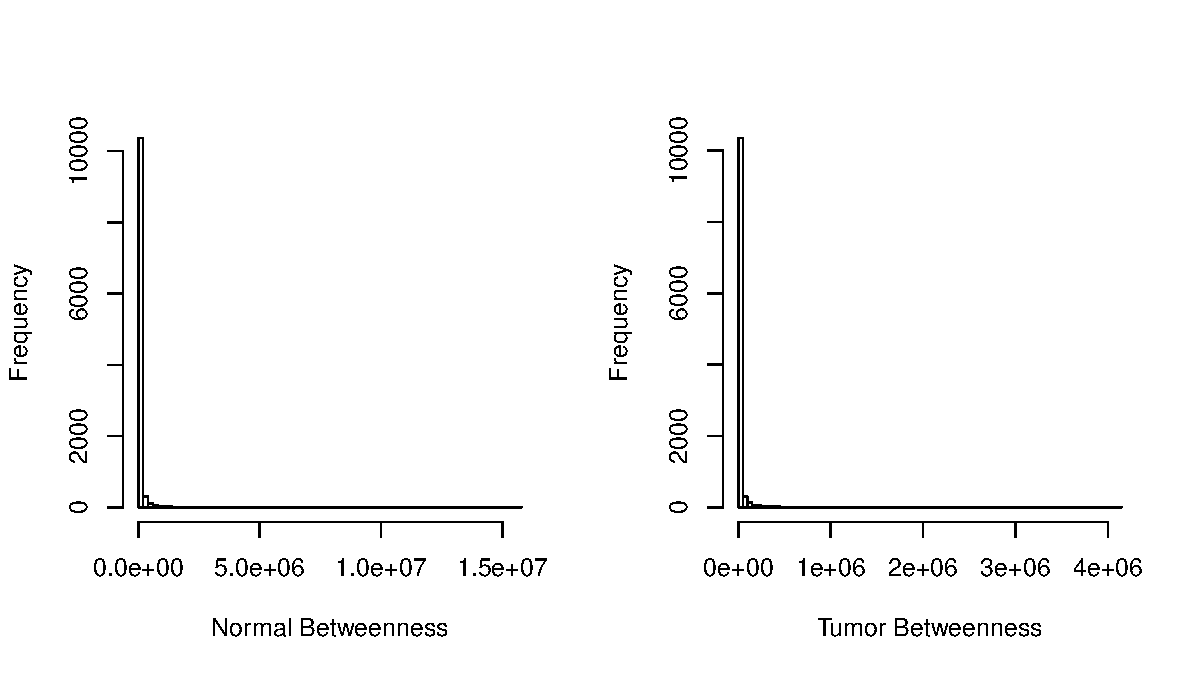
\includegraphics[width=\maxwidth]{figure/unnamed-chunk-9-1} 

\end{knitrout}

\begin{center}
\small{Figure 1a and 1b (left to right): Histograms of the betweenness centrality values for the normal and tumor data. Both are drastically skewed right.}
\end{center}

Below are the summaries for the normal and tumor betweenness values.
\begin{knitrout}\small
\definecolor{shadecolor}{rgb}{0.969, 0.969, 0.969}\color{fgcolor}\begin{kframe}
\begin{alltt}
\hlkwd{summary}\hlstd{(NB)}
\end{alltt}
\begin{verbatim}
##  Normal Betweenness
##  Min.   :       0  
##  1st Qu.:       0  
##  Median :       0  
##  Mean   :  104182  
##  3rd Qu.:    6757  
##  Max.   :15702357
\end{verbatim}
\begin{alltt}
\hlkwd{summary}\hlstd{(TB)}
\end{alltt}
\begin{verbatim}
##  Tumor Betweenness
##  Min.   :      0  
##  1st Qu.:     15  
##  Median :    327  
##  Mean   :  17577  
##  3rd Qu.:   3613  
##  Max.   :4116666
\end{verbatim}
\end{kframe}
\end{knitrout}
The normal data has a much larger betweenness value than the tumor data. Out of 11055 genes, 7500 genes have a betweenness value of 0 in the normal data, and 2130 genes have that value in the tumor data. This implies that 67.8$\%$ and 19.3$\%$ of the genes in the normal and tumor data can be made in this network without the aid of any intermediary gene. Additionally, 75$\%$ of genes have a betweenness value less than 5598 and 3556 in the normal and tumor data. Therefore, only a few genes have betweenness value that tend towards the maximum values, which imply that these are the ``high-trafic" nodes in the network.


Figure 1 is a plot of the normal versus tumor betweenness values.


\begin{knitrout}\small
\definecolor{shadecolor}{rgb}{0.969, 0.969, 0.969}\color{fgcolor}\begin{kframe}
\begin{alltt}
\hlcom{# creating a dataframe that has both expression & betweeness data}
\hlcom{# both sets have the same genes, so names should match up}

\hlstd{norm_central} \hlkwb{=} \hlkwd{cbind}\hlstd{(NB)} \hlcom{# grab betweeness}
\hlstd{tumor_central} \hlkwb{=} \hlkwd{cbind}\hlstd{(TB)} \hlcom{# grab betweeness for tumor}
\hlstd{centrality_data} \hlkwb{=} \hlkwd{cbind}\hlstd{(norm_central, tumor_central)} \hlcom{# hold betweeness for norm and tumor}


\hlstd{indx} \hlkwb{<-} \hlkwd{which}\hlstd{(}\hlkwd{row.names}\hlstd{(norm_data)} \hlopt \hlkwd{row.names}\hlstd{(norm_central))} \hlcom{# grab indices of genes in both sets}
\hlstd{norm_avg} \hlkwb{<-} \hlkwd{as.matrix}\hlstd{(}\hlkwd{rowMeans}\hlstd{(norm_data[indx,]))} \hlcom{# average the values across the row for each gene}
\hlkwd{colnames}\hlstd{(norm_avg)} \hlkwb{<-} \hlkwd{c}\hlstd{(}\hlstr{'Normal Avg'}\hlstd{)}
\hlkwd{rownames}\hlstd{(norm_avg)} \hlkwb{=} \hlkwd{row.names}\hlstd{(norm_data)[indx]}


\hlstd{indx} \hlkwb{<-} \hlkwd{which}\hlstd{(}\hlkwd{row.names}\hlstd{(tumor_data)} \hlopt \hlkwd{row.names}\hlstd{(tumor_central))} \hlcom{# grab indices of genes in both sets}
\hlstd{tumor_avg} \hlkwb{<-} \hlkwd{as.matrix}\hlstd{(}\hlkwd{rowMeans}\hlstd{(tumor_data[indx,]))} \hlcom{# average the values across the row for each gene}
\hlkwd{colnames}\hlstd{(tumor_avg)} \hlkwb{<-} \hlkwd{c}\hlstd{(}\hlstr{'Tumor Avg'}\hlstd{)}
\hlkwd{rownames}\hlstd{(tumor_avg)} \hlkwb{=} \hlkwd{row.names}\hlstd{(tumor_data)[indx]}


\hlcom{# re-arrange to match the same gene order as the centrality data}
\hlstd{norm_avg}  \hlkwb{=} \hlkwd{as.matrix}\hlstd{(norm_avg[}\hlkwd{row.names}\hlstd{(centrality_data),])}
\hlstd{tumor_avg} \hlkwb{=} \hlkwd{as.matrix}\hlstd{(tumor_avg[}\hlkwd{row.names}\hlstd{(centrality_data),])}
\hlkwd{colnames}\hlstd{(norm_avg)} \hlkwb{<-} \hlkwd{c}\hlstd{(}\hlstr{'Normal Avg'}\hlstd{)}
\hlkwd{colnames}\hlstd{(tumor_avg)} \hlkwb{<-} \hlkwd{c}\hlstd{(}\hlstr{'Tumor Avg'}\hlstd{)}


\hlcom{# calculate fold-change values}
\hlstd{fc} \hlkwb{<-} \hlstd{tumor_avg}\hlopt{/}\hlstd{norm_avg}
\hlkwd{colnames}\hlstd{(fc)} \hlkwb{<-} \hlkwd{c}\hlstd{(}\hlstr{'FC Value'}\hlstd{)}


\hlcom{# calculate ratio of tumor to normal betweenness}
\hlstd{ratio_b} \hlkwb{<-} \hlkwd{as.matrix}\hlstd{(centrality_data[,}\hlnum{2}\hlstd{]}\hlopt{/}\hlstd{centrality_data[,}\hlnum{1}\hlstd{])}
\hlkwd{colnames}\hlstd{(ratio_b)} \hlkwb{<-} \hlkwd{c}\hlstd{(}\hlstr{'T_B/N_B'}\hlstd{)}

\hlcom{# store centrality measures, rpkm, and fc values in one place}
\hlstd{data_plot} \hlkwb{=} \hlkwd{cbind}\hlstd{(centrality_data, norm_avg, tumor_avg, fc, ratio_b)}

\hlcom{# set threshold #1}
\hlstd{nb_thresh} \hlkwb{=} \hlnum{1000000}
\hlstd{tb_thresh} \hlkwb{=} \hlnum{1000000}
\hlstd{indx} \hlkwb{<-} \hlkwd{which}\hlstd{(data_plot[,}\hlnum{1}\hlstd{]} \hlopt{>=} \hlstd{nb_thresh} \hlopt{|} \hlstd{data_plot[,}\hlnum{2}\hlstd{]} \hlopt{>=} \hlstd{tb_thresh)} \hlcom{# grab genes who meet one of the cutoff marks}
\hlstd{data_thresh} \hlkwb{=} \hlkwd{as.matrix}\hlstd{(data_plot[indx,])} \hlcom{# grab genes }


\hlcom{# set threshold #2}
\hlstd{indx} \hlkwb{<-} \hlkwd{which}\hlstd{(data_thresh[,}\hlnum{6}\hlstd{]} \hlopt{>=} \hlnum{1.1}\hlstd{)} \hlcom{# grab indices of genes whose ratio is >= 2}
\hlstd{data_thresh} \hlkwb{=} \hlkwd{as.matrix}\hlstd{(data_thresh[indx,])} \hlcom{# grab genes }

\hlkwd{tiff}\hlstd{(}\hlstr{"Fig3.tiff"}\hlstd{,} \hlkwc{width} \hlstd{=} \hlnum{6}\hlstd{,} \hlkwc{height} \hlstd{=} \hlnum{5}\hlstd{,} \hlkwc{units} \hlstd{=} \hlstr{'in'}\hlstd{,} \hlkwc{res} \hlstd{=} \hlnum{800}\hlstd{)}
\hlkwd{plot}\hlstd{(data_plot[,}\hlnum{1}\hlstd{], data_plot[,}\hlnum{2}\hlstd{],} \hlkwc{xlab} \hlstd{=} \hlstr{"Normal Betweenness"}\hlstd{,} \hlkwc{ylab} \hlstd{=} \hlstr{"Tumor Betweenness"}\hlstd{,} \hlkwc{col} \hlstd{=} \hlstr{'black'}\hlstd{,} \hlkwc{pch} \hlstd{=} \hlnum{1}\hlstd{,} \hlkwc{xlim} \hlstd{=} \hlkwd{c}\hlstd{(}\hlnum{0}\hlstd{,}\hlnum{18000000}\hlstd{),} \hlkwc{ylim} \hlstd{=} \hlkwd{c}\hlstd{(}\hlnum{0}\hlstd{,}\hlnum{5000000}\hlstd{))}
\hlkwd{par}\hlstd{(}\hlkwc{new}\hlstd{=}\hlnum{TRUE}\hlstd{)}
\hlkwd{plot}\hlstd{(data_thresh[,}\hlnum{1}\hlstd{], data_thresh[,}\hlnum{2}\hlstd{],} \hlkwc{xlab} \hlstd{=} \hlstr{"Normal Betweenness"}\hlstd{,} \hlkwc{ylab} \hlstd{=} \hlstr{"Tumor Betweenness"}\hlstd{,} \hlkwc{col} \hlstd{=} \hlstr{'red'}\hlstd{,} \hlkwc{pch} \hlstd{=} \hlnum{16}\hlstd{,}  \hlkwc{main} \hlstd{=} \hlnum{NA}\hlstd{,} \hlkwc{xlim} \hlstd{=} \hlkwd{c}\hlstd{(}\hlnum{0}\hlstd{,}\hlnum{18000000}\hlstd{),} \hlkwc{ylim} \hlstd{=} \hlkwd{c}\hlstd{(}\hlnum{0}\hlstd{,}\hlnum{5000000}\hlstd{))}
\hlkwd{dev.off}\hlstd{()}
\end{alltt}
\begin{verbatim}
## pdf 
##   2
\end{verbatim}
\begin{alltt}
\hlkwd{jpeg}\hlstd{(}\hlstr{"Fig3.jpeg"}\hlstd{,} \hlkwc{width} \hlstd{=} \hlnum{6}\hlstd{,} \hlkwc{height} \hlstd{=} \hlnum{5}\hlstd{,} \hlkwc{units} \hlstd{=} \hlstr{'in'}\hlstd{,} \hlkwc{res} \hlstd{=} \hlnum{800}\hlstd{)}
\hlkwd{plot}\hlstd{(data_plot[,}\hlnum{1}\hlstd{], data_plot[,}\hlnum{2}\hlstd{],} \hlkwc{xlab} \hlstd{=} \hlstr{"Normal Betweenness"}\hlstd{,} \hlkwc{ylab} \hlstd{=} \hlstr{"Tumor Betweenness"}\hlstd{,} \hlkwc{col} \hlstd{=} \hlstr{'black'}\hlstd{,} \hlkwc{pch} \hlstd{=} \hlnum{1}\hlstd{,} \hlkwc{xlim} \hlstd{=} \hlkwd{c}\hlstd{(}\hlnum{0}\hlstd{,}\hlnum{18000000}\hlstd{),} \hlkwc{ylim} \hlstd{=} \hlkwd{c}\hlstd{(}\hlnum{0}\hlstd{,}\hlnum{5000000}\hlstd{))}
\hlkwd{par}\hlstd{(}\hlkwc{new}\hlstd{=}\hlnum{TRUE}\hlstd{)}
\hlkwd{plot}\hlstd{(data_thresh[,}\hlnum{1}\hlstd{], data_thresh[,}\hlnum{2}\hlstd{],} \hlkwc{xlab} \hlstd{=} \hlstr{"Normal Betweenness"}\hlstd{,} \hlkwc{ylab} \hlstd{=} \hlstr{"Tumor Betweenness"}\hlstd{,} \hlkwc{col} \hlstd{=} \hlstr{'red'}\hlstd{,} \hlkwc{pch} \hlstd{=} \hlnum{16}\hlstd{,}  \hlkwc{main} \hlstd{=} \hlnum{NA}\hlstd{,} \hlkwc{xlim} \hlstd{=} \hlkwd{c}\hlstd{(}\hlnum{0}\hlstd{,}\hlnum{18000000}\hlstd{),} \hlkwc{ylim} \hlstd{=} \hlkwd{c}\hlstd{(}\hlnum{0}\hlstd{,}\hlnum{5000000}\hlstd{))}
\hlkwd{dev.off}\hlstd{()}
\end{alltt}
\begin{verbatim}
## pdf 
##   2
\end{verbatim}
\begin{alltt}
\hlstd{indx} \hlkwb{=} \hlkwd{which}\hlstd{(}\hlkwd{rownames}\hlstd{(NC)} \hlopt \hlkwd{rownames}\hlstd{(data_thresh))}

\hlkwd{tiff}\hlstd{(}\hlstr{"Fig4.tiff"}\hlstd{,} \hlkwc{width} \hlstd{=} \hlnum{6}\hlstd{,} \hlkwc{height} \hlstd{=} \hlnum{5}\hlstd{,} \hlkwc{units} \hlstd{=} \hlstr{'in'}\hlstd{,} \hlkwc{res} \hlstd{=} \hlnum{800}\hlstd{)}
\hlkwd{plot}\hlstd{(NC[,}\hlnum{1}\hlstd{], TC[,}\hlnum{1}\hlstd{],} \hlkwc{xlab} \hlstd{=} \hlstr{"Normal Closeness"}\hlstd{,} \hlkwc{ylab} \hlstd{=} \hlstr{"Tumor Closeness"}\hlstd{,} \hlkwc{col} \hlstd{=} \hlstr{'black'}\hlstd{,} \hlkwc{pch} \hlstd{=} \hlnum{1}\hlstd{,} \hlkwc{xlim} \hlstd{=} \hlkwd{c}\hlstd{(}\hlnum{0}\hlstd{,}\hlnum{0.0025}\hlstd{),} \hlkwc{ylim} \hlstd{=} \hlkwd{c}\hlstd{(}\hlnum{0.00004}\hlstd{,}\hlnum{0.00016}\hlstd{))}
\hlkwd{par}\hlstd{(}\hlkwc{new}\hlstd{=}\hlnum{TRUE}\hlstd{)}
\hlkwd{plot}\hlstd{(NC[indx,}\hlnum{1}\hlstd{], TC[indx,}\hlnum{1}\hlstd{],} \hlkwc{xlab} \hlstd{=} \hlstr{"Normal Closeness"}\hlstd{,} \hlkwc{ylab} \hlstd{=} \hlstr{"Tumor Closeness"}\hlstd{,} \hlkwc{col} \hlstd{=} \hlstr{'red'}\hlstd{,} \hlkwc{pch} \hlstd{=} \hlnum{16}\hlstd{,}  \hlkwc{main} \hlstd{=} \hlnum{NA}\hlstd{,} \hlkwc{xlim} \hlstd{=} \hlkwd{c}\hlstd{(}\hlnum{0}\hlstd{,}\hlnum{0.0025}\hlstd{),} \hlkwc{ylim} \hlstd{=} \hlkwd{c}\hlstd{(}\hlnum{0.00004}\hlstd{,}\hlnum{0.00016}\hlstd{))}
\hlkwd{dev.off}\hlstd{()}
\end{alltt}
\begin{verbatim}
## pdf 
##   2
\end{verbatim}
\begin{alltt}
\hlkwd{jpeg}\hlstd{(}\hlstr{"Fig4.jpeg"}\hlstd{,} \hlkwc{width} \hlstd{=} \hlnum{6}\hlstd{,} \hlkwc{height} \hlstd{=} \hlnum{5}\hlstd{,} \hlkwc{units} \hlstd{=} \hlstr{'in'}\hlstd{,} \hlkwc{res} \hlstd{=} \hlnum{800}\hlstd{)}
\hlkwd{plot}\hlstd{(NC[,}\hlnum{1}\hlstd{], TC[,}\hlnum{1}\hlstd{],} \hlkwc{xlab} \hlstd{=} \hlstr{"Normal Closeness"}\hlstd{,} \hlkwc{ylab} \hlstd{=} \hlstr{"Tumor Closeness"}\hlstd{,} \hlkwc{col} \hlstd{=} \hlstr{'black'}\hlstd{,} \hlkwc{pch} \hlstd{=} \hlnum{1}\hlstd{,} \hlkwc{xlim} \hlstd{=} \hlkwd{c}\hlstd{(}\hlnum{0}\hlstd{,}\hlnum{0.0025}\hlstd{),} \hlkwc{ylim} \hlstd{=} \hlkwd{c}\hlstd{(}\hlnum{0.00004}\hlstd{,}\hlnum{0.00016}\hlstd{))}
\hlkwd{par}\hlstd{(}\hlkwc{new}\hlstd{=}\hlnum{TRUE}\hlstd{)}
\hlkwd{plot}\hlstd{(NC[indx,}\hlnum{1}\hlstd{], TC[indx,}\hlnum{1}\hlstd{],} \hlkwc{xlab} \hlstd{=} \hlstr{"Normal Closeness"}\hlstd{,} \hlkwc{ylab} \hlstd{=} \hlstr{"Tumor Closeness"}\hlstd{,} \hlkwc{col} \hlstd{=} \hlstr{'red'}\hlstd{,} \hlkwc{pch} \hlstd{=} \hlnum{16}\hlstd{,}  \hlkwc{main} \hlstd{=} \hlnum{NA}\hlstd{,} \hlkwc{xlim} \hlstd{=} \hlkwd{c}\hlstd{(}\hlnum{0}\hlstd{,}\hlnum{0.0025}\hlstd{),} \hlkwc{ylim} \hlstd{=} \hlkwd{c}\hlstd{(}\hlnum{0.00004}\hlstd{,}\hlnum{0.00016}\hlstd{))}
\hlkwd{dev.off}\hlstd{()}
\end{alltt}
\begin{verbatim}
## pdf 
##   2
\end{verbatim}
\end{kframe}
\end{knitrout}
\begin{figure}
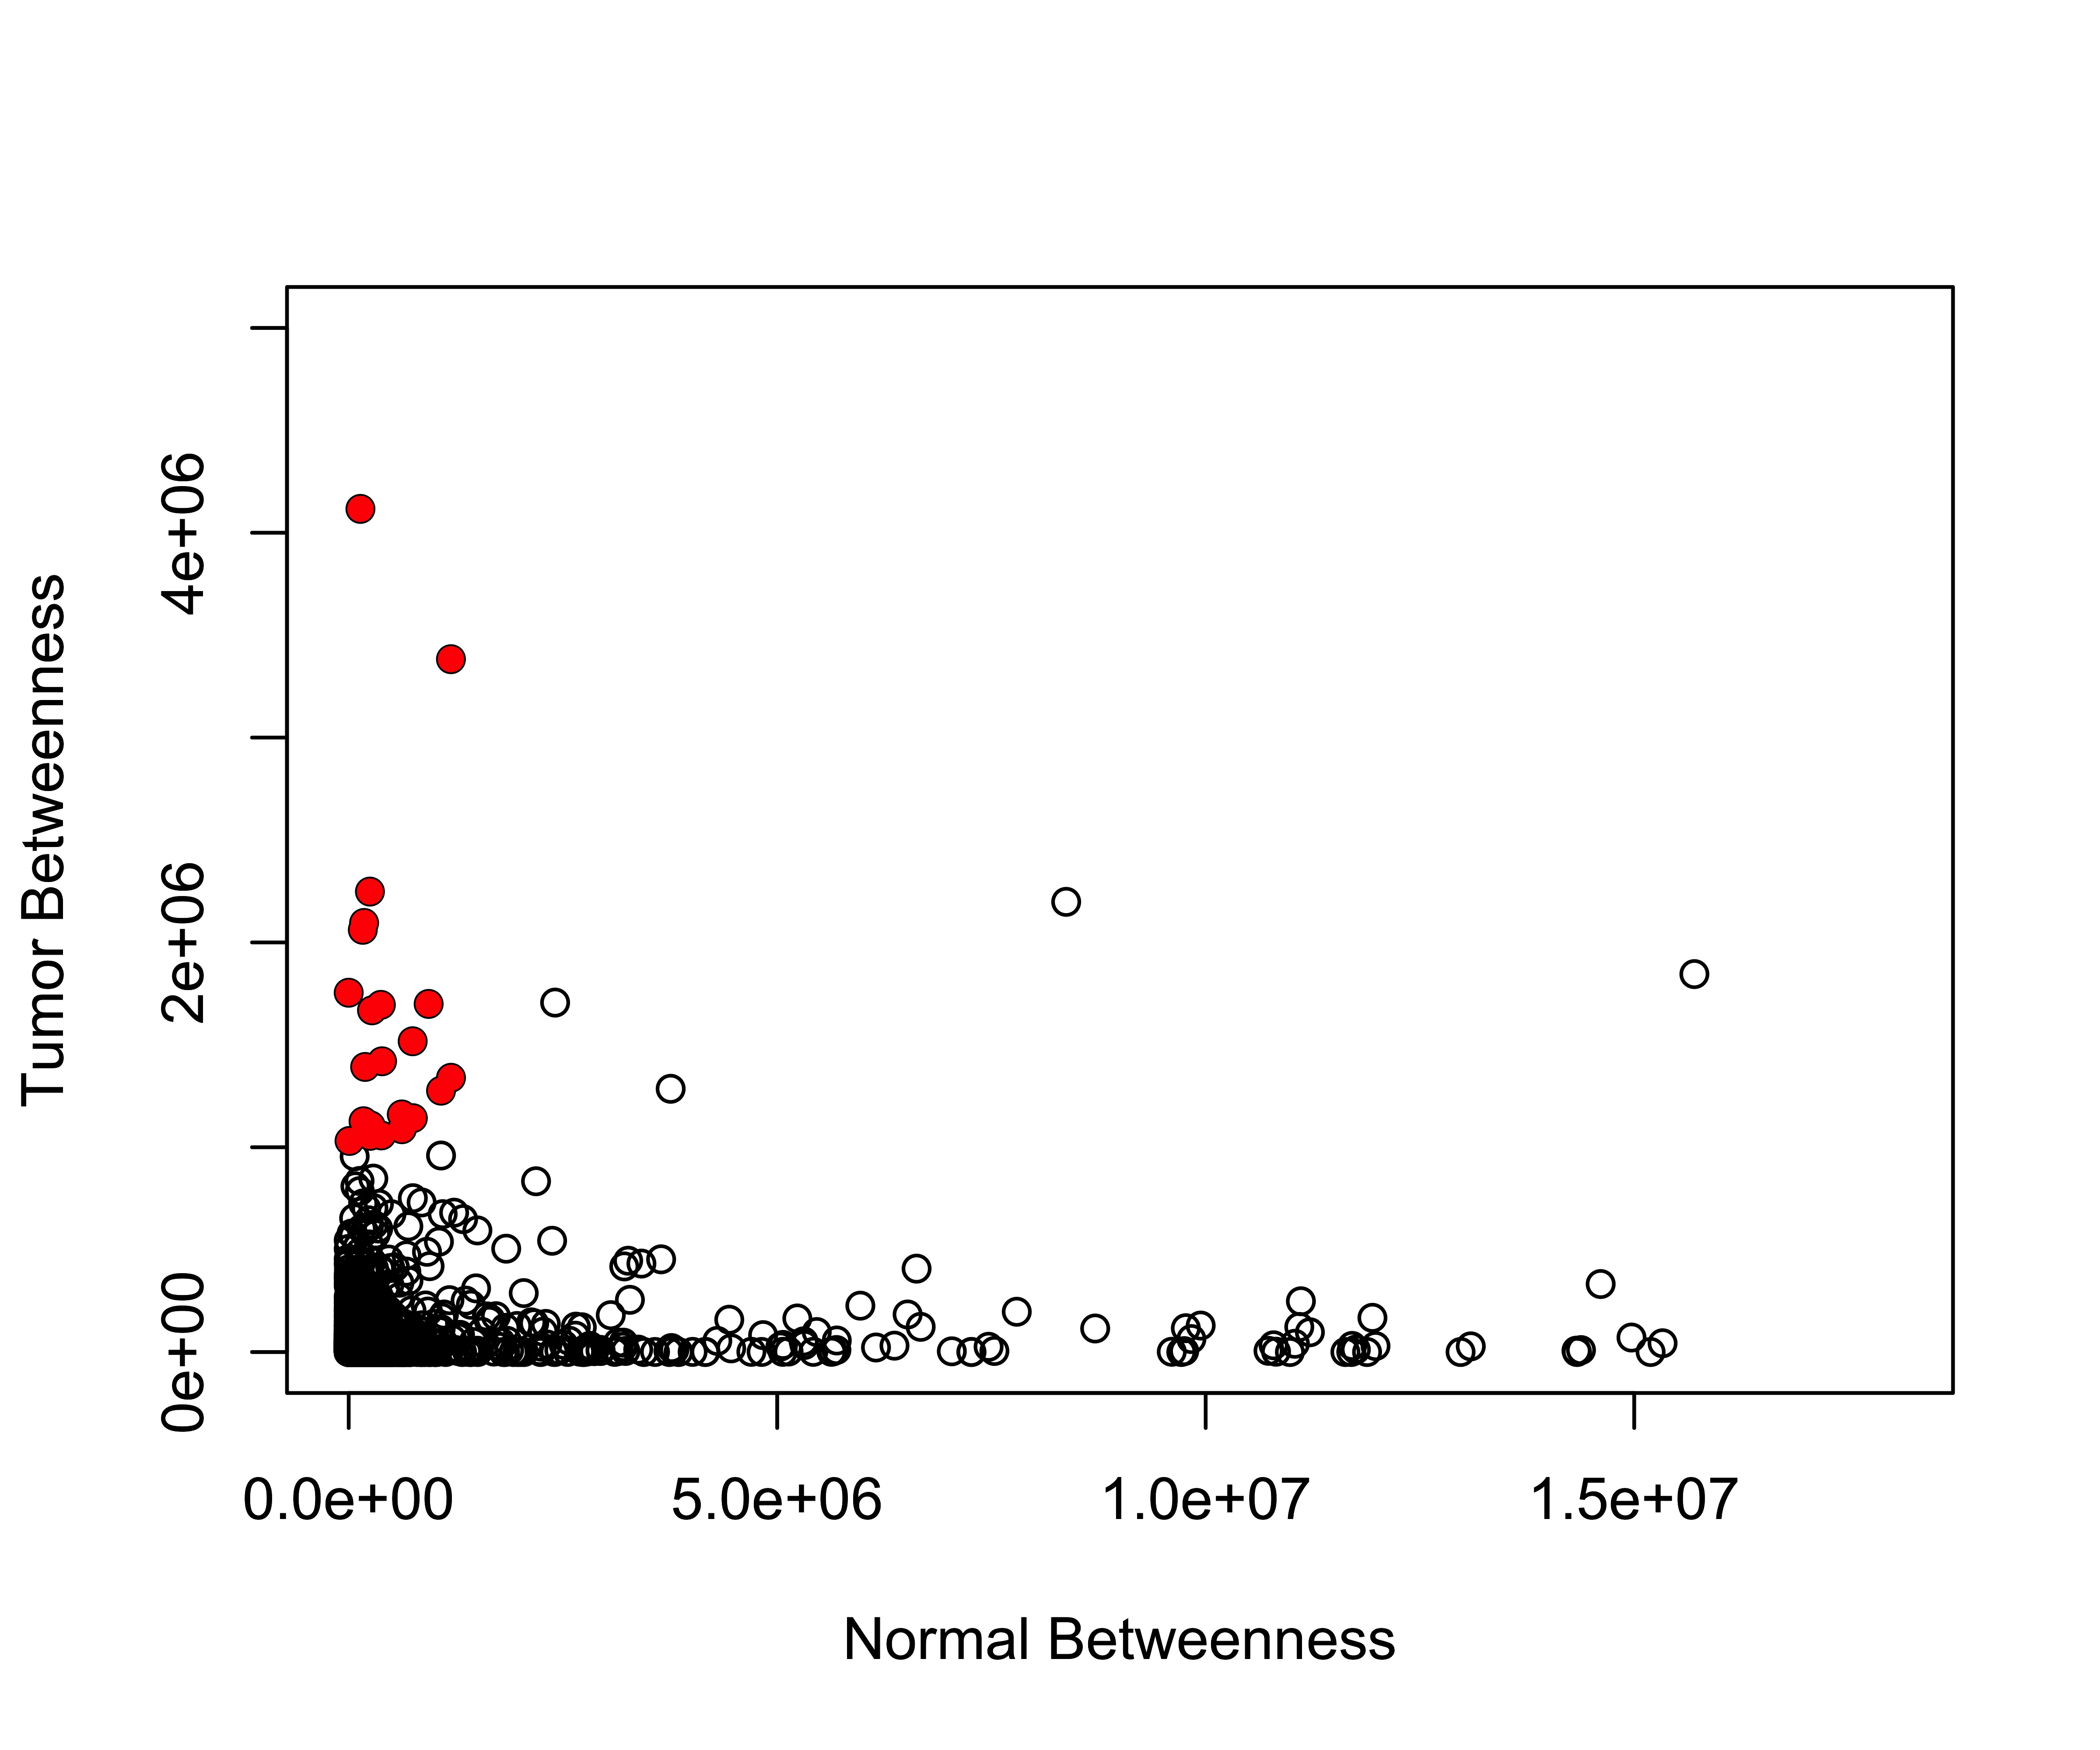
\includegraphics[scale=.1]{Fig3.jpeg}
\caption{Betweenness plot of the genes.}
\end{figure}

\begin{figure}
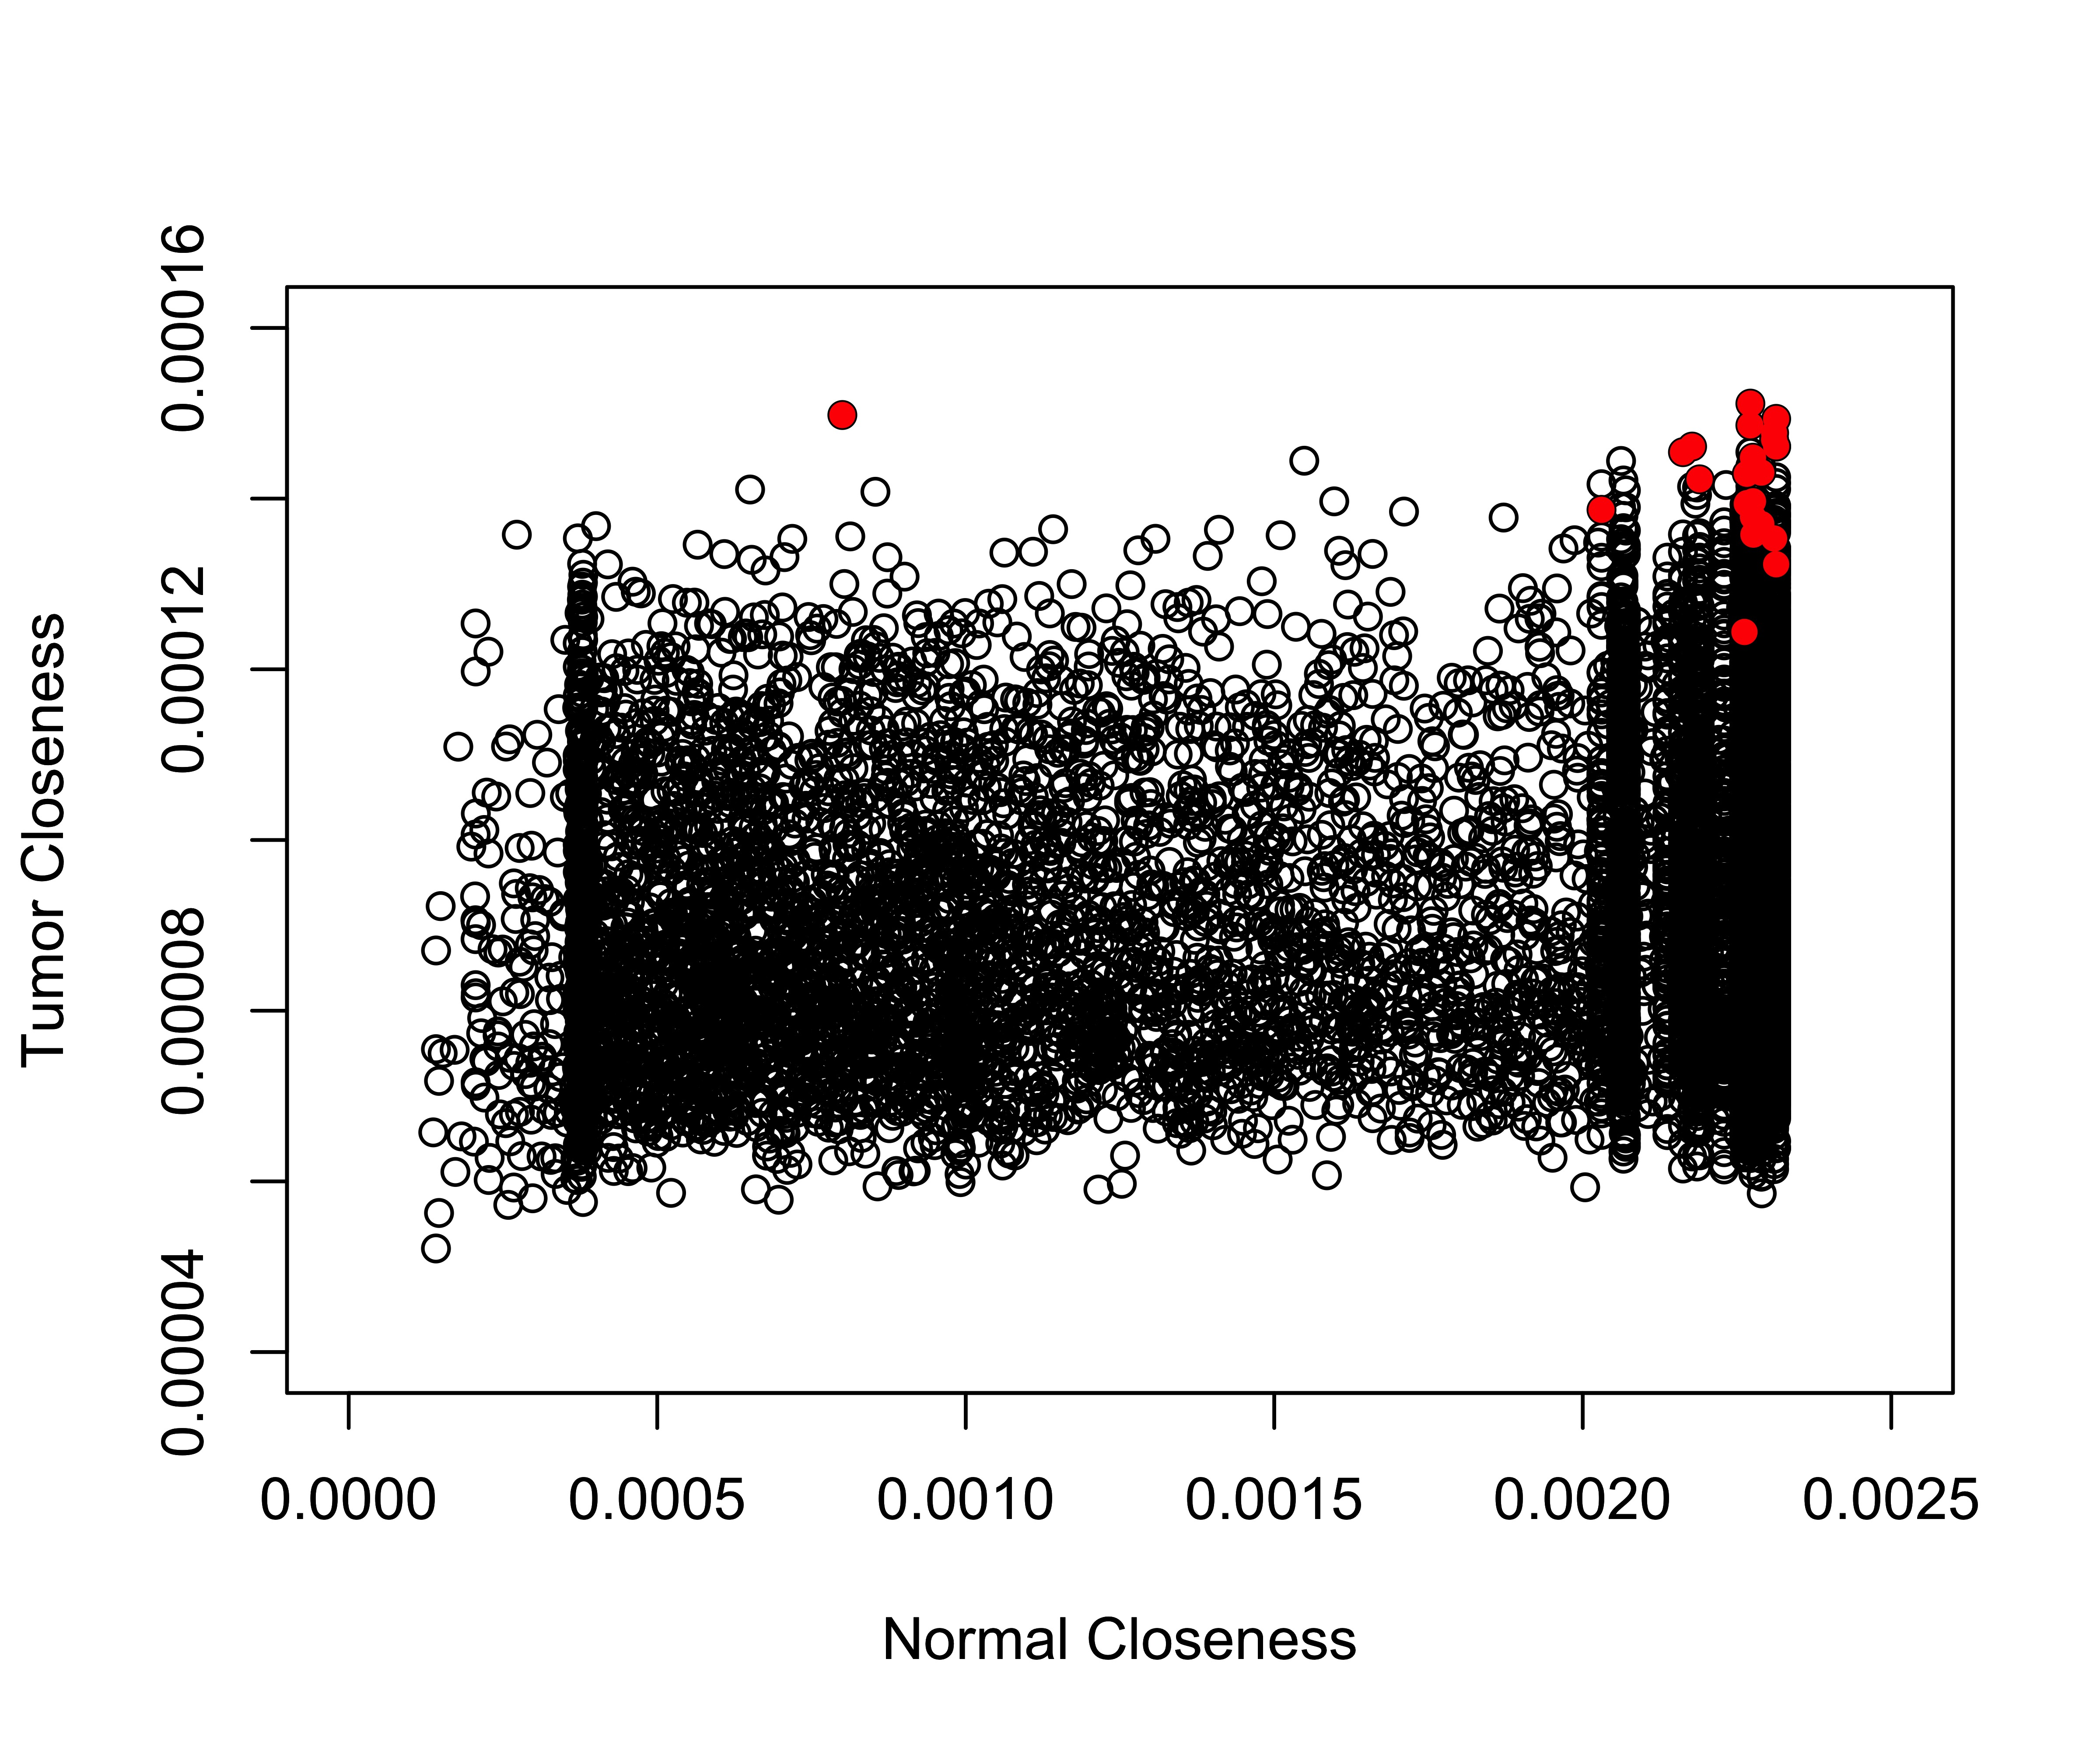
\includegraphics[scale=.1]{Fig4.jpeg}
\caption{Closeness plot of the genes.}
\end{figure}

We are interested in the genes which have a betweenness ratio of 1.1:1, meaning its tumor betweenness value is at least 1.1 as big as its normal betweenness value. The genes we are concerned are colored red in Figure 3 and are
\begin{knitrout}\small
\definecolor{shadecolor}{rgb}{0.969, 0.969, 0.969}\color{fgcolor}\begin{kframe}
\begin{alltt}
\hlkwd{row.names}\hlstd{(data_thresh)}
\end{alltt}
\begin{verbatim}
##  [1] "CEBPZ"   "ETV5"    "SPEN"    "ZCCHC14" "CAMTA1"  "CHD5"    "CERS2"  
##  [8] "HNRNPAB" "ILF2"    "ZCCHC17" "ZC3H15"  "TULP4"   "PURB"    "RPL7"   
## [15] "TCF3"    "TEAD1"   "CNBP"    "PRDM2"   "SARNP"   "ZRANB2"  "GCSH"   
## [22] "IFT74"   "MYL12B"
\end{verbatim}
\end{kframe}
\end{knitrout}


Those 23 genes are colored in red in the plots in Figure 1, which highlights the betweenness values of the normal and tumor sets. The same 23 genes are colored in red in Figure 2, which highlights the WNC values (I think WNC just means closeness, but I'm not sure...  ???) of the normal and tumor sets. Note that the scale in Figure 2 are adjusted by multiplying the WNC values by the standard error of each set, $\sqrt(4)$ for the normal data and $\sqrt(11)$ for the tumor data.


%%%%%%%%%%%%%%%%%%%%%%%%%%%%%%%%%%%%%%%%%%%%%%%%%%%%%%%%%%%%%%%%%%%%%%%%%%%%%
%%%%%%%%%%%%%%%%%%%%%%%%%%%%%%%%%%%%%%%%%%%%%%%%%%%%%%%%%%%%%%%%%%%%%%%%%%%%%
%%%%%%%%%%%%%%%%%%%%%%%%%%%%%%%%%%%%%%%%%%%%%%%%%%%%%%%%%%%%%%%%%%%%%%%%%%%%%
%%%%%%%%%%%%%%%%%%%%%%%%%%%%%%%%%%%%%%%%%%%%%%%%%%%%%%%%%%%%%%%%%%%%%%%%%%%%%


\newpage
\section{ETV5 Differential Expression}

The goal of this analysis is to understand the differential expression of the genes which are {\em regulated} by genes identified in a previous analysis.  At this stage, we are using only one dataset:  Optic Glioma.  There are 4 normal mice samples and 11 tumor mice samples.


\subsection{Previously identified genes}
The process for identifying \textcolor{red}{regulator} genes is as follows:

\begin{enumerate}
\item
Use interactome network as provided by Peter Sims (binary and directional relationships between 13089 genes).
\item
For the weights along the interactome network, use 1-abs(cor) for a dissimilarity metric (using expression data).  Find the new weighted network for each of the tumor and normal datasets.
\item
Extract a sub-network using genes which are highest according to the betweeness complexity measure.  For each dataset, there will be 2 sub-networks (one normal and one tumor).  [Be sure to intersect the genes in the two lists for an apples to apples comparison.]
\item
Compare normal and tumor sub-networks in each dataset.
\end{enumerate}

The genes which were identified as most promising are the following:  

\begin{knitrout}\small
\definecolor{shadecolor}{rgb}{0.969, 0.969, 0.969}\color{fgcolor}\begin{kframe}
\begin{alltt}
\hlkwd{row.names}\hlstd{(data_thresh)}
\end{alltt}
\begin{verbatim}
##  [1] "CEBPZ"   "ETV5"    "SPEN"    "ZCCHC14" "CAMTA1"  "CHD5"    "CERS2"  
##  [8] "HNRNPAB" "ILF2"    "ZCCHC17" "ZC3H15"  "TULP4"   "PURB"    "RPL7"   
## [15] "TCF3"    "TEAD1"   "CNBP"    "PRDM2"   "SARNP"   "ZRANB2"  "GCSH"   
## [22] "IFT74"   "MYL12B"
\end{verbatim}
\end{kframe}
\end{knitrout}

\subsection{Finding target genes}

As mentioned, the original interactome network from Peter Sims contains the relationships between genes.  For each of the regulators, we find the list of upstream genes.
\begin{knitrout}\small
\definecolor{shadecolor}{rgb}{0.969, 0.969, 0.969}\color{fgcolor}\begin{kframe}
\begin{alltt}
\hlstd{possibleRegulators} \hlkwb{=} \hlkwd{row.names}\hlstd{(data_thresh)}
\end{alltt}
\end{kframe}
\end{knitrout}

\begin{knitrout}\small
\definecolor{shadecolor}{rgb}{0.969, 0.969, 0.969}\color{fgcolor}\begin{kframe}
\begin{alltt}
\hlcom{# Read in network.  }
\hlstd{intNet}\hlkwb{=}\hlkwd{read.table}\hlstd{(}\hlstr{"gbm-sun-interactome.txt"}\hlstd{,}\hlkwc{header}\hlstd{=}\hlnum{TRUE}\hlstd{,}\hlkwc{sep}\hlstd{=}\hlstr{"\textbackslash{}t"}\hlstd{)}

\hlstd{tarGenes} \hlkwb{=} \hlkwd{list}\hlstd{()}
\hlkwa{for}\hlstd{(i} \hlkwa{in} \hlnum{1}\hlopt{:}\hlkwd{length}\hlstd{(possibleRegulators))\{}
  \hlstd{tarGenes[[i]]} \hlkwb{=} \hlkwd{t}\hlstd{(}\hlkwd{data.frame}\hlstd{(}\hlkwd{lapply}\hlstd{(intNet[intNet[,}\hlnum{1}\hlstd{]}\hlopt{==}\hlstd{possibleRegulators[i],}\hlnum{2}\hlstd{],as.character),}
                               \hlkwc{stringsAsFactors} \hlstd{=} \hlnum{FALSE}\hlstd{))}
 \hlkwa{if}\hlstd{(}\hlkwd{nrow}\hlstd{(tarGenes[[i]])} \hlopt{>} \hlnum{0}\hlstd{) \{}\hlkwd{colnames}\hlstd{(tarGenes[[i]])} \hlkwb{=} \hlkwd{c}\hlstd{(}\hlstr{"GENE"}\hlstd{)}
 \hlstd{tarGenes[[i]]} \hlkwb{=} \hlkwd{data.frame}\hlstd{(tarGenes[[i]])\}}
\hlstd{\}}
\hlkwd{names}\hlstd{(tarGenes)} \hlkwb{=} \hlkwd{as.vector}\hlstd{(possibleRegulators)}
\end{alltt}
\end{kframe}
\end{knitrout}

\begin{knitrout}\scriptsize
\definecolor{shadecolor}{rgb}{0.969, 0.969, 0.969}\color{fgcolor}\begin{kframe}
\begin{alltt}
\hlcom{# The number of target genes for each of the possible regulators:}
\hlkwd{lapply}\hlstd{(tarGenes,nrow)}
\end{alltt}
\begin{verbatim}
## $CEBPZ
## [1] 416
## 
## $ETV5
## [1] 504
## 
## $SPEN
## [1] 443
## 
## $ZCCHC14
## [1] 402
## 
## $CAMTA1
## [1] 1210
## 
## $CHD5
## [1] 950
## 
## $CERS2
## [1] 570
## 
## $HNRNPAB
## [1] 608
## 
## $ILF2
## [1] 613
## 
## $ZCCHC17
## [1] 286
## 
## $ZC3H15
## [1] 735
## 
## $TULP4
## [1] 460
## 
## $PURB
## [1] 783
## 
## $RPL7
## [1] 280
## 
## $TCF3
## [1] 732
## 
## $TEAD1
## [1] 498
## 
## $CNBP
## [1] 522
## 
## $PRDM2
## [1] 730
## 
## $SARNP
## [1] 317
## 
## $ZRANB2
## [1] 559
## 
## $GCSH
## [1] 0
## 
## $IFT74
## [1] 0
## 
## $MYL12B
## [1] 0
\end{verbatim}
\end{kframe}
\end{knitrout}

\begin{knitrout}\small
\definecolor{shadecolor}{rgb}{0.969, 0.969, 0.969}\color{fgcolor}\begin{kframe}
\begin{alltt}
\hlcom{# the number of genes described in the interactome network: }
\hlkwd{length}\hlstd{(}\hlkwd{unique}\hlstd{(intNet[,}\hlnum{1}\hlstd{]))}  \hlcom{# number of unique regulators}
\end{alltt}
\begin{verbatim}
## [1] 1265
\end{verbatim}
\begin{alltt}
\hlkwd{length}\hlstd{(}\hlkwd{unique}\hlstd{(intNet[,}\hlnum{2}\hlstd{]))}  \hlcom{# number of unique targets}
\end{alltt}
\begin{verbatim}
## [1] 11824
\end{verbatim}
\begin{alltt}
\hlkwd{length}\hlstd{(}\hlkwd{unique}\hlstd{(}\hlkwd{union}\hlstd{(intNet[,}\hlnum{1}\hlstd{], intNet[,}\hlnum{2}\hlstd{])))} \hlcom{# number of unique transcriptomes total}
\end{alltt}
\begin{verbatim}
## [1] 13089
\end{verbatim}
\end{kframe}
\end{knitrout}

For good measure, it is interesting to see which of the regulators are also differentially expressed.  (Only ETV5!  The genes are sorted based on the adjusted p-value.)

\begin{knitrout}\small
\definecolor{shadecolor}{rgb}{0.969, 0.969, 0.969}\color{fgcolor}\begin{kframe}
\begin{alltt}
\hlstd{DEanalysis} \hlkwb{=} \hlstd{miceps} \hlcom{# the DE analysis from normalization above}
\hlstd{DEps} \hlkwb{=} \hlstd{DEanalysis[,}\hlkwd{c}\hlstd{(}\hlstr{"gene"}\hlstd{,} \hlstr{"pvalue"}\hlstd{,} \hlstr{"padj"}\hlstd{,} \hlstr{"log2FoldChange"}\hlstd{)]}
\hlstd{DEps} \hlkwb{=} \hlstd{DEps} \hlopt \hlkwd{mutate}\hlstd{(}\hlkwc{GENE}\hlstd{=gene)} \hlopt \hlstd{dplyr}\hlopt{::}\hlkwd{select}\hlstd{(}\hlopt{-}\hlstd{gene)}
\hlcom{#head(DEps)}

\hlstd{regGenesP} \hlkwb{<-} \hlkwd{left_join}\hlstd{(}\hlkwd{data.frame}\hlstd{(}\hlkwc{GENE} \hlstd{= possibleRegulators), DEps,} \hlkwc{by}\hlstd{=}\hlstr{"GENE"}\hlstd{)}
\hlstd{regGenesP} \hlopt \hlkwd{arrange}\hlstd{(padj)}
\end{alltt}
\begin{verbatim}
##       GENE   pvalue     padj log2FoldChange
## 1     ETV5 1.34e-09 3.87e-07         1.4474
## 2   MYL12B 6.81e-04 1.61e-02        -0.5850
## 3   ZC3H15 4.03e-03 5.12e-02        -0.5603
## 4   CAMTA1 4.22e-03 5.24e-02        -0.4705
## 5     SPEN 4.61e-03 5.55e-02         0.5714
## 6    TULP4 6.11e-03 6.48e-02         0.4845
## 7    SARNP 7.36e-03 7.24e-02        -0.7022
## 8  ZCCHC17 9.34e-03 8.26e-02        -0.6699
## 9    IFT74 9.66e-03 8.43e-02        -0.5475
## 10    TCF3 1.29e-02 9.89e-02         0.4928
## 11 ZCCHC14 3.82e-02 1.80e-01         0.3660
## 12    RPL7 3.83e-02 1.80e-01        -0.5100
## 13    CNBP 4.16e-02 1.88e-01        -0.3724
## 14  ZRANB2 6.71e-02 2.47e-01        -0.3515
## 15   TEAD1 1.40e-01 3.70e-01         0.2794
## 16    ILF2 1.51e-01 3.83e-01        -0.3077
## 17   CEBPZ 1.60e-01 3.96e-01        -0.3255
## 18    GCSH 3.92e-01 6.38e-01        -0.1581
## 19   CERS2 5.36e-01 7.49e-01        -0.0923
## 20 HNRNPAB 6.23e-01 8.06e-01         0.0784
## 21    PURB 6.80e-01 8.43e-01         0.0573
## 22   PRDM2 8.75e-01 9.45e-01         0.0207
## 23    CHD5 8.98e-01 9.57e-01        -0.0334
\end{verbatim}
\end{kframe}
\end{knitrout}

\newpage
\subsection*{DE for target genes}

A DESeq anlaysis was done on the optic glioma dataset using DESeq2.  

\begin{knitrout}\small
\definecolor{shadecolor}{rgb}{0.969, 0.969, 0.969}\color{fgcolor}\begin{kframe}
\begin{alltt}
\hlstd{tarGenesP} \hlkwb{=} \hlkwd{list}\hlstd{()}
\hlkwa{for}\hlstd{(i} \hlkwa{in} \hlnum{1}\hlopt{:}\hlkwd{length}\hlstd{(possibleRegulators))\{}
  \hlstd{temp} \hlkwb{=} \hlstd{tarGenes[[i]]}
  \hlkwa{if}\hlstd{(}\hlkwd{nrow}\hlstd{(temp)} \hlopt{>} \hlnum{0}\hlstd{) tarGenesP[[i]]} \hlkwb{<-} \hlkwd{left_join}\hlstd{(temp, DEps,} \hlkwc{by}\hlstd{=} \hlstr{"GENE"}\hlstd{)}
  \hlkwa{if}\hlstd{(}\hlkwd{nrow}\hlstd{(temp)} \hlopt{==} \hlnum{0}\hlstd{) tarGenesP[[i]]} \hlkwb{<-} \hlkwd{data.frame}\hlstd{(}\hlkwc{GENE}\hlstd{=}\hlnum{NA}\hlstd{,} \hlkwc{pvalue}\hlstd{=}\hlnum{NA}\hlstd{,} \hlkwc{padj}\hlstd{=}\hlnum{NA}\hlstd{,} \hlkwc{log2FoldChange}\hlstd{=}\hlnum{NA}\hlstd{)}
\hlstd{\}}
\hlkwd{names}\hlstd{(tarGenesP)} \hlkwb{=} \hlkwd{as.vector}\hlstd{(possibleRegulators)}

\hlstd{siglevel} \hlkwb{=} \hlnum{0.01}
\hlstd{numsig} \hlkwb{=} \hlkwd{sapply}\hlstd{(tarGenesP,} \hlkwa{function}\hlstd{(}\hlkwc{x}\hlstd{)} \hlkwd{sum}\hlstd{(x}\hlopt{$}\hlstd{padj} \hlopt{<} \hlstd{siglevel,} \hlkwc{na.rm}\hlstd{=T))}
\hlstd{totalps} \hlkwb{=} \hlkwd{sapply}\hlstd{(tarGenesP,} \hlkwa{function}\hlstd{(}\hlkwc{x}\hlstd{)} \hlkwd{sum}\hlstd{(}\hlopt{!}\hlkwd{is.na}\hlstd{(x}\hlopt{$}\hlstd{padj)))}
\hlstd{percsig} \hlkwb{=} \hlkwd{sapply}\hlstd{(tarGenesP,} \hlkwa{function}\hlstd{(}\hlkwc{x}\hlstd{)} \hlkwd{sum}\hlstd{(x}\hlopt{$}\hlstd{padj} \hlopt{<} \hlstd{siglevel,} \hlkwc{na.rm}\hlstd{=T))} \hlopt{/} \hlkwd{sapply}\hlstd{(tarGenesP,} \hlkwa{function}\hlstd{(}\hlkwc{x}\hlstd{)} \hlkwd{sum}\hlstd{(}\hlopt{!}\hlkwd{is.na}\hlstd{(x}\hlopt{$}\hlstd{padj)))}

\hlstd{all} \hlkwb{=} \hlkwd{data.frame}\hlstd{(}\hlkwc{numsig}\hlstd{=}\hlkwd{sum}\hlstd{(DEps}\hlopt{$}\hlstd{padj} \hlopt{<} \hlstd{siglevel,} \hlkwc{na.rm}\hlstd{=T),}
                 \hlkwc{totalps} \hlstd{=} \hlkwd{sum}\hlstd{(}\hlopt{!}\hlkwd{is.na}\hlstd{(DEps}\hlopt{$}\hlstd{padj)),}
                 \hlkwc{percsig} \hlstd{=} \hlkwd{sum}\hlstd{(DEps}\hlopt{$}\hlstd{padj} \hlopt{<} \hlstd{siglevel,} \hlkwc{na.rm}\hlstd{=T)}\hlopt{/}\hlkwd{sum}\hlstd{(}\hlopt{!}\hlkwd{is.na}\hlstd{(DEps}\hlopt{$}\hlstd{padj)))}
\hlstd{TargetPs} \hlkwb{=} \hlkwd{cbind}\hlstd{(}\hlkwc{GENE}\hlstd{=}\hlkwd{c}\hlstd{(}\hlkwd{names}\hlstd{(numsig),}\hlstr{"ALL"}\hlstd{),}\hlkwd{rbind}\hlstd{(}\hlkwd{data.frame}\hlstd{(numsig,totalps,percsig),} \hlkwc{all}\hlstd{=all))}
\end{alltt}
\end{kframe}
\end{knitrout}

\subsubsection{Visualizing p-values}

\begin{knitrout}\small
\definecolor{shadecolor}{rgb}{0.969, 0.969, 0.969}\color{fgcolor}\begin{kframe}
\begin{alltt}
\hlstd{numReg} \hlkwb{=} \hlkwd{length}\hlstd{(possibleRegulators)}
\hlkwd{par}\hlstd{(}\hlkwc{mfrow}\hlstd{=}\hlkwd{c}\hlstd{(}\hlnum{1}\hlstd{,}\hlnum{2}\hlstd{))}
\hlkwd{hist}\hlstd{(DEps}\hlopt{$}\hlstd{pvalue,} \hlkwc{main}\hlstd{=}\hlstr{"all genes"}\hlstd{,} \hlkwc{xlab}\hlstd{=}\hlstr{"raw p-value"}\hlstd{,} \hlkwc{ylab}\hlstd{=}\hlstr{"Freq"}\hlstd{)}
\hlkwd{hist}\hlstd{(DEps}\hlopt{$}\hlstd{padj,} \hlkwc{main}\hlstd{=}\hlstr{"all genes"}\hlstd{,} \hlkwc{xlab}\hlstd{=}\hlstr{"adjusted p-value"}\hlstd{,} \hlkwc{ylab}\hlstd{=}\hlstr{"Freq"}\hlstd{)}
\end{alltt}
\end{kframe}
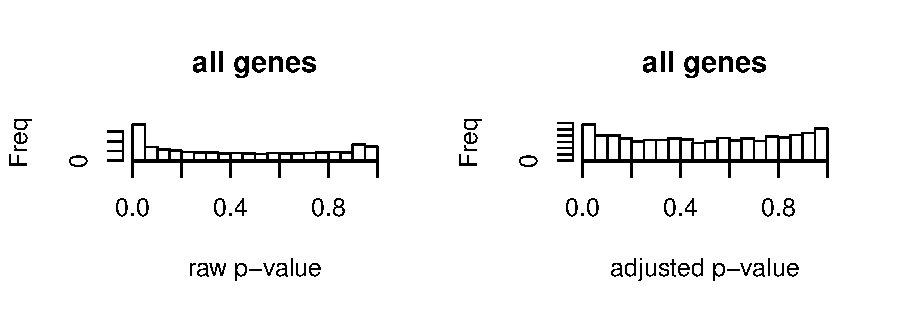
\includegraphics[width=\maxwidth]{figure/unnamed-chunk-20-1} 
\begin{kframe}\begin{alltt}
\hlcom{# only printing for ETV5, uncomment to see all sig genes for all regulators}
\hlcom{# for(i in 1:numReg)\{}
\hlcom{#  if(sum(!is.na(tarGenesP[[i]]$pvalue)) > 0)\{}
\hlcom{#  hist(tarGenesP[[i]]$pvalue, main=possibleRegulators[i], xlab="raw p-value", ylab="Freq")}
\hlcom{#  hist(tarGenesP[[i]]$padj, main=possibleRegulators[i], xlab="adjusted p-value", ylab="Freq")\}}
\hlcom{#\}}

\hlkwd{hist}\hlstd{(tarGenesP[}\hlstr{"ETV5"}\hlstd{]}\hlopt{$}\hlstd{ETV5}\hlopt{$}\hlstd{pvalue,} \hlkwc{main}\hlstd{=}\hlstr{"ETV5"}\hlstd{,} \hlkwc{xlab}\hlstd{=}\hlstr{"raw p-value"}\hlstd{,} \hlkwc{ylab}\hlstd{=}\hlstr{"Freq"}\hlstd{)}
\hlkwd{hist}\hlstd{(tarGenesP[}\hlstr{"ETV5"}\hlstd{]}\hlopt{$}\hlstd{ETV5}\hlopt{$}\hlstd{padj,} \hlkwc{main}\hlstd{=}\hlstr{"ETV5"}\hlstd{,} \hlkwc{xlab}\hlstd{=}\hlstr{"adjusted p-value"}\hlstd{,} \hlkwc{ylab}\hlstd{=}\hlstr{"Freq"}\hlstd{)}
\end{alltt}
\end{kframe}
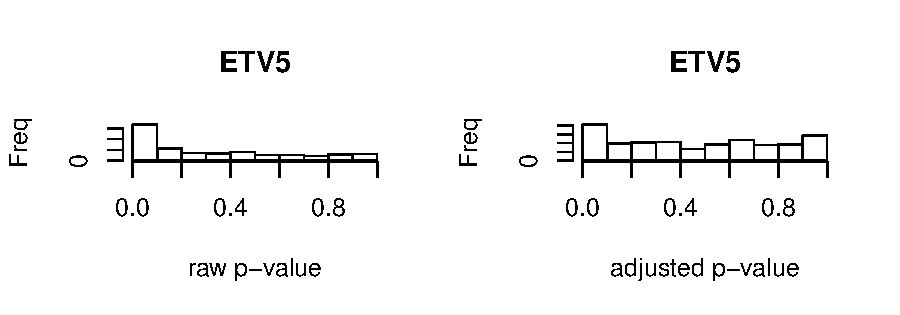
\includegraphics[width=\maxwidth]{figure/unnamed-chunk-20-2} 
\begin{kframe}\begin{alltt}
\hlcom{#prints summary of pvalues for all regulators of interest:}
\hlcom{#lapply(tarGenesP,function(x) summary(x[,-1]))}

\hlcom{#significance level is 0.01 (for adjusted p-value)}
\hlcom{#ordered by the percent of significant targets, ETV5 is highest}
\hlstd{TargetPs}  \hlopt \hlkwd{arrange}\hlstd{(}\hlkwd{desc}\hlstd{(percsig))}
\end{alltt}
\begin{verbatim}
##       GENE numsig totalps percsig
## 1     ETV5     31     449  0.0690
## 2    CERS2     32     496  0.0645
## 3    SARNP     15     255  0.0588
## 4  ZCCHC14     16     361  0.0443
## 5     TCF3     28     640  0.0437
## 6    TEAD1     19     443  0.0429
## 7   ZC3H15     27     652  0.0414
## 8    TULP4     17     412  0.0413
## 9     RPL7     10     247  0.0405
## 10    PURB     27     678  0.0398
## 11     ALL    529   14926  0.0354
## 12 HNRNPAB     19     543  0.0350
## 13    CNBP     15     458  0.0328
## 14  CAMTA1     35    1093  0.0320
## 15    CHD5     27     852  0.0317
## 16 ZCCHC17      8     257  0.0311
## 17   PRDM2     20     652  0.0307
## 18    SPEN     12     392  0.0306
## 19   CEBPZ     10     379  0.0264
## 20    ILF2     13     555  0.0234
## 21  ZRANB2     11     486  0.0226
## 22    GCSH      0       0     NaN
## 23   IFT74      0       0     NaN
## 24  MYL12B      0       0     NaN
\end{verbatim}
\end{kframe}
\end{knitrout}

\vspace*{-.5cm}
\subsubsection{Lists of Significant Genes}

\begin{knitrout}\small
\definecolor{shadecolor}{rgb}{0.969, 0.969, 0.969}\color{fgcolor}\begin{kframe}
\begin{alltt}
\hlcom{# only printing for ETV5, uncomment to see all sig genes for all regulators}
\hlcom{# lapply(tarGenesP, function(x) x[c(x$padj < siglevel & !is.na(x$padj)),])}
\hlstd{tarGenesP}\hlopt{$}\hlstd{ETV5[}\hlkwd{c}\hlstd{(tarGenesP}\hlopt{$}\hlstd{ETV5}\hlopt{$}\hlstd{padj} \hlopt{<} \hlstd{siglevel} \hlopt{& !}\hlkwd{is.na}\hlstd{(tarGenesP}\hlopt{$}\hlstd{ETV5}\hlopt{$}\hlstd{padj)),]}
\end{alltt}
\begin{verbatim}
##         GENE   pvalue     padj log2FoldChange
## 16     SPRY2 1.13e-08 2.41e-06          0.916
## 38    DNAJB4 2.63e-05 1.65e-03         -0.457
## 64    COL2A1 1.07e-04 4.43e-03          1.235
## 91    SPRED1 1.04e-05 7.78e-04          0.800
## 102    DUSP6 1.50e-04 5.54e-03          0.637
## 104    S1PR1 6.84e-17 9.28e-14          1.358
## 110      AK4 5.38e-05 2.77e-03          0.959
## 115    FABP5 1.39e-09 3.93e-07          1.087
## 116    FABP7 6.22e-05 3.02e-03          0.956
## 127   RSBN1L 2.16e-04 7.15e-03         -0.428
## 132    BTBD3 7.12e-09 1.62e-06          0.755
## 172    GAP43 1.94e-05 1.27e-03         -0.797
## 183     GJA1 3.64e-10 1.26e-07          0.600
## 188     GLDC 6.60e-06 5.29e-04          1.161
## 201   KCNIP1 3.06e-04 9.09e-03         -0.797
## 212   IGFBP6 3.07e-04 9.10e-03         -0.942
## 232     LRP4 5.38e-05 2.77e-03          0.671
## 239    MMP15 2.11e-04 7.07e-03          1.003
## 255     NT5E 1.18e-04 4.76e-03         -0.744
## 260  PCDHGC3 2.12e-06 2.09e-04          0.932
## 278    TPPP3 6.01e-05 2.94e-03         -0.912
## 291     SHC3 2.71e-04 8.35e-03          0.903
## 295    NLGN3 1.82e-05 1.21e-03          0.705
## 300   SPATA6 1.62e-04 5.86e-03         -0.552
## 302   ELOVL2 1.62e-11 9.28e-09          1.908
## 437    SPRY4 5.77e-05 2.87e-03          1.104
## 466    SOCS2 1.77e-04 6.28e-03         -0.814
## 483 SLC9A3R1 1.41e-06 1.51e-04          0.722
## 486    CHST2 2.28e-11 1.26e-08          1.163
## 490   CXCL14 4.88e-17 7.29e-14          1.425
## 496    DOCK4 2.88e-05 1.73e-03          0.642
\end{verbatim}
\end{kframe}
\end{knitrout}

%%%%%%%%%%%%%%%%%%%%%%%%%%%%%%%%%%%%%%%%%%%%%%%%%%%%%%%%%%%%%%%%%%%%%%%%%%%%%
%%%%%%%%%%%%%%%%%%%%%%%%%%%%%%%%%%%%%%%%%%%%%%%%%%%%%%%%%%%%%%%%%%%%%%%%%%%%%
%%%%%%%%%%%%%%%%%%%%%%%%%%%%%%%%%%%%%%%%%%%%%%%%%%%%%%%%%%%%%%%%%%%%%%%%%%%%%
%%%%%%%%%%%%%%%%%%%%%%%%%%%%%%%%%%%%%%%%%%%%%%%%%%%%%%%%%%%%%%%%%%%%%%%%%%%%%

\newpage
\section{Public Data - Human}

\subsection{Data}
The following analysis is further investigation into ETV5 using two human datasets.  

\subsubsection{GSE42656 Study}
\url{https://www.ncbi.nlm.nih.gov/geo/query/acc.cgi?acc=GSE42656}\\
\url{http://cancerres.aacrjournals.org/content/73/18/5834.long#sec-2}\\
Henriquez NV et al., ``Comparative expression analysis reveals lineage relationships between human and murine gliomas and a dominance of glial signatures during tumor propagation in vitro.'', {\bf Cancer Res}, 2013 Jul 25;73(18):5834-44\\


{\bf From NCBI data repository} \\
``We analysed gene expression in paediatric brain tumours as compared to normal adult brain in order to understand the molecular profiles. Our cohort included 14 pilocytic astrocytomas, 3 diffuse astrocytomas, 2 anaplastic astrocytomas, 5 glioblastomas, 14 ependymomas, 9 medulloblastomas, 5 atypical teratoid/rhabdoid tumours, 4 choroid plexus papillomas, 1 papillary glioneuronal, 8 adult brain and 8 foetal brain controls.''\\

{\bf Article Abstract:}\\
Brain tumors are thought to originate from stem/progenitor cell populations that acquire specific genetic mutations. Although current preclinical models have relevance to human pathogenesis, most do not recapitulate the histogenesis of the human disease. Recently, a large series of human gliomas and medulloblastomas were analyzed for genetic signatures of prognosis and therapeutic response. Using a mouse model system that generates three distinct types of intrinsic brain tumors, we correlated RNA and protein expression levels with human brain tumors. A combination of genetic mutations and cellular environment during tumor propagation defined the incidence and phenotype of intrinsic murine tumors. Importantly, in vitro passage of cancer stem cells uniformly promoted a glial expression profile in culture and in brain tumors. Gene expression profiling revealed that experimental gliomas corresponded to distinct subclasses of human glioblastoma, whereas experimental supratentorial primitive neuroectodermal tumors (sPNET) correspond to atypical teratoid/rhabdoid tumor (AT/RT), a rare childhood tumor.\\

{\bf Methods:} Human samples using Ilumina arrays (Illumina HT12$\_$v3).



\subsubsection{GSE12907 Study}

Need to fill in the references / experimental design / methods for the GSE12907 dataset.

This data set has 21 juvenile pilocytic astrocytoma samples (columns 2-22), three samples from normal cerebellum (from humans ages 8, 16 and 63, columns 23-25), and one normal foetal sample (column 26).  The first column contains the Probe IDs.


\subsubsection{Data Wrangling of both datasets}

\begin{knitrout}\small
\definecolor{shadecolor}{rgb}{0.969, 0.969, 0.969}\color{fgcolor}\begin{kframe}
\begin{alltt}
\hlcom{#targets of ETV5 only}
\hlstd{tarGenesETV5} \hlkwb{<-} \hlstd{tarGenesP}\hlopt{$}\hlstd{ETV5}

\hlcom{# inputting the two human datasets}
\hlstd{GSE42656} \hlkwb{<-} \hlkwd{read.delim}\hlstd{(}\hlstr{"GSE42656_series_dataonly.txt"}\hlstd{,} \hlkwc{sep}\hlstd{=}\hlstr{"\textbackslash{}t"}\hlstd{)}
\hlstd{GSE12907} \hlkwb{<-} \hlkwd{read.delim}\hlstd{(}\hlstr{"GSE12907_series_dataonly.txt"}\hlstd{,} \hlkwc{sep}\hlstd{=}\hlstr{"\textbackslash{}t"}\hlstd{)}
\hlstd{ETV5name} \hlkwb{<-} \hlkwd{data.frame}\hlstd{(}\hlkwc{GENE}\hlstd{=}\hlstr{"ETV5"}\hlstd{)}

\hlstd{PROBES.GSE42656} \hlkwb{<-} \hlkwd{as.character}\hlstd{(GSE42656}\hlopt{$}\hlstd{ID_REF)}  \hlcom{# Illumina}
\hlstd{PROBES.GSE12907} \hlkwb{<-} \hlkwd{as.character}\hlstd{(GSE12907}\hlopt{$}\hlstd{ID_REF)}  \hlcom{# Affymetrix Human Genome U133A}

\hlstd{IlluminaIDs} \hlkwb{<-} \hlstd{AnnotationDbi}\hlopt{::}\hlkwd{select}\hlstd{(illuminaHumanv4.db, PROBES.GSE42656,} \hlkwd{c}\hlstd{(}\hlstr{"SYMBOL"}\hlstd{,}\hlstr{"PROBEID"}\hlstd{,} \hlstr{"ENTREZID"}\hlstd{,} \hlstr{"GENENAME"}\hlstd{))}
\hlstd{AffyIDs} \hlkwb{<-} \hlstd{AnnotationDbi}\hlopt{::}\hlkwd{select}\hlstd{(hgu133plus2.db, PROBES.GSE12907,} \hlkwd{c}\hlstd{(}\hlstr{"SYMBOL"}\hlstd{,}\hlstr{"PROBEID"}\hlstd{,} \hlstr{"ENTREZID"}\hlstd{,} \hlstr{"GENENAME"}\hlstd{))}


\hlcom{# cleaning up GSE42656}
\hlstd{pilocytic} \hlkwb{<-} \hlkwd{c}\hlstd{(}\hlstr{"GSM1047395"}\hlstd{,} \hlstr{"GSM1047396"}\hlstd{,} \hlstr{"GSM1047397"}\hlstd{,} \hlstr{"GSM1047399"}\hlstd{,} \hlstr{"GSM1047400"}\hlstd{,}
               \hlstr{"GSM1047401"}\hlstd{,} \hlstr{"GSM1047402"}\hlstd{,} \hlstr{"GSM1047403"}\hlstd{,} \hlstr{"GSM1047404"}\hlstd{,} \hlstr{"GSM1047405"}\hlstd{,}
               \hlstr{"GSM1047406"}\hlstd{,} \hlstr{"GSM1047407"}\hlstd{,} \hlstr{"GSM1047408"}\hlstd{,} \hlstr{"GSM1047409"}\hlstd{)}

\hlstd{foetal} \hlkwb{<-} \hlkwd{c}\hlstd{(}\hlstr{"GSM1047452"}\hlstd{,}       \hlstr{"GSM1047453"}\hlstd{,}   \hlstr{"GSM1047454"}\hlstd{,}   \hlstr{"GSM1047455"}\hlstd{,}   \hlstr{"GSM1047456"}\hlstd{,}
            \hlstr{"GSM1047457"}\hlstd{,}       \hlstr{"GSM1047458"}\hlstd{,}   \hlstr{"GSM1047459"}\hlstd{)}

\hlcom{# ETV5_GSE42656 - FOETAL}
\hlstd{ETV5_GSE42656} \hlkwb{<-} \hlstd{GSE42656} \hlopt
  \hlstd{dplyr}\hlopt{::}\hlkwd{select}\hlstd{(}\hlkwd{one_of}\hlstd{(}\hlkwd{c}\hlstd{(}\hlstr{"ID_REF"}\hlstd{, pilocytic, foetal)))} \hlopt
  \hlkwd{left_join}\hlstd{(IlluminaIDs,} \hlkwc{by} \hlstd{=} \hlkwd{c}\hlstd{(}\hlstr{"ID_REF"} \hlstd{=} \hlstr{"PROBEID"}\hlstd{))} \hlopt
  \hlkwd{right_join}\hlstd{(ETV5name,} \hlkwc{by}\hlstd{=}\hlkwd{c}\hlstd{(}\hlstr{"SYMBOL"}\hlstd{=} \hlstr{"GENE"}\hlstd{))} \hlopt
  \hlstd{dplyr}\hlopt{::}\hlkwd{select}\hlstd{(}\hlopt{-}\hlstd{ENTREZID,} \hlopt{-}\hlstd{GENENAME)}

\hlstd{ETV5_GSE42656_tidy} \hlkwb{<-} \hlstd{ETV5_GSE42656} \hlopt
  \hlstd{tidyr}\hlopt{::}\hlkwd{gather}\hlstd{(sampleID, expression,} \hlopt{-}\hlkwd{c}\hlstd{(ID_REF,SYMBOL))} \hlopt
  \hlkwd{mutate}\hlstd{(}\hlkwc{expression} \hlstd{=} \hlkwd{parse_number}\hlstd{(expression))} \hlopt
  \hlkwd{mutate}\hlstd{(}\hlkwc{sample} \hlstd{=} \hlkwd{ifelse}\hlstd{(sampleID} \hlopt \hlstd{pilocytic,} \hlstr{"pilocytic"}\hlstd{,} \hlstr{"foetal"}\hlstd{))}


\hlstd{AffyIDs} \hlkwb{<-} \hlstd{AnnotationDbi}\hlopt{::}\hlkwd{select}\hlstd{(hgu133plus2.db, PROBES.GSE12907,}  \hlkwd{c}\hlstd{(}\hlstr{"SYMBOL"}\hlstd{,} \hlstr{"ENTREZID"}\hlstd{,} \hlstr{"GENENAME"}\hlstd{))}

\hlstd{CBM} \hlkwb{=} \hlkwd{colnames}\hlstd{(GSE12907)[}\hlnum{23}\hlopt{:}\hlnum{26}\hlstd{]}
\hlstd{pilocytic12907} \hlkwb{=} \hlkwd{colnames}\hlstd{(GSE12907)[}\hlnum{2}\hlopt{:}\hlnum{22}\hlstd{]}

\hlcom{# ETV5_GSE12907 }
\hlstd{ETV5_GSE12907} \hlkwb{<-} \hlstd{GSE12907} \hlopt
  \hlkwd{left_join}\hlstd{(AffyIDs,} \hlkwc{by} \hlstd{=} \hlkwd{c}\hlstd{(}\hlstr{"ID_REF"} \hlstd{=} \hlstr{"PROBEID"}\hlstd{))} \hlopt
  \hlkwd{right_join}\hlstd{(ETV5name,} \hlkwc{by}\hlstd{=}\hlkwd{c}\hlstd{(}\hlstr{"SYMBOL"}\hlstd{=} \hlstr{"GENE"}\hlstd{))} \hlopt
  \hlstd{dplyr}\hlopt{::}\hlkwd{select}\hlstd{(}\hlopt{-}\hlstd{ENTREZID,} \hlopt{-}\hlstd{GENENAME)}

\hlstd{ETV5_GSE12907_tidy} \hlkwb{<-} \hlstd{ETV5_GSE12907} \hlopt
  \hlstd{tidyr}\hlopt{::}\hlkwd{gather}\hlstd{(sampleID, expression,} \hlopt{-}\hlkwd{c}\hlstd{(ID_REF,SYMBOL))} \hlopt
  \hlkwd{mutate}\hlstd{(}\hlkwc{expression} \hlstd{=} \hlkwd{parse_number}\hlstd{(expression))} \hlopt
  \hlkwd{mutate}\hlstd{(}\hlkwc{sample} \hlstd{=} \hlkwd{ifelse}\hlstd{(sampleID} \hlopt \hlstd{CBM,} \hlstr{"CBM"}\hlstd{,} \hlstr{"PA"}\hlstd{))}
\end{alltt}
\end{kframe}
\end{knitrout}



\subsection{t-tests on ETV5 for both datasets}

\begin{knitrout}\small
\definecolor{shadecolor}{rgb}{0.969, 0.969, 0.969}\color{fgcolor}\begin{kframe}
\begin{alltt}
\hlcom{#ETV5_GSE42656}
\hlkwa{for}\hlstd{(i} \hlkwa{in} \hlnum{1}\hlopt{:}\hlkwd{nrow}\hlstd{(ETV5_GSE42656))\{}
\hlkwd{print}\hlstd{(}\hlkwd{t.test}\hlstd{(ETV5_GSE42656[i,}\hlnum{2}\hlopt{:}\hlnum{15}\hlstd{], ETV5_GSE42656[i,}\hlnum{16}\hlopt{:}\hlnum{23}\hlstd{]))}
\hlstd{\}}
\end{alltt}
\begin{verbatim}
## 
## 	Welch Two Sample t-test
## 
## data:  ETV5_GSE42656[i, 2:15] and ETV5_GSE42656[i, 16:23]
## t = 4, df = 20, p-value = 8e-04
## alternative hypothesis: true difference in means is not equal to 0
## 95 percent confidence interval:
##  20.8 64.5
## sample estimates:
## mean of x mean of y 
##       175       133 
## 
## 
## 	Welch Two Sample t-test
## 
## data:  ETV5_GSE42656[i, 2:15] and ETV5_GSE42656[i, 16:23]
## t = 6, df = 20, p-value = 4e-06
## alternative hypothesis: true difference in means is not equal to 0
## 95 percent confidence interval:
##   900 1762
## sample estimates:
## mean of x mean of y 
##      2521      1190
\end{verbatim}
\begin{alltt}
\hlstd{ETV5_GSE42656_tidy} \hlkwb{<-} \hlstd{ETV5_GSE42656_tidy} \hlopt
  \hlkwd{mutate}\hlstd{(}\hlkwc{sample2} \hlstd{=} \hlkwd{ifelse}\hlstd{(sample}\hlopt{==}\hlstr{"foetal"}\hlstd{,} \hlstr{"control"}\hlstd{,} \hlstr{"PA"}\hlstd{))}

\hlkwd{ggplot}\hlstd{(ETV5_GSE42656_tidy,} \hlkwd{aes}\hlstd{(}\hlkwc{y}\hlstd{=expression,} \hlkwc{x}\hlstd{=sample))} \hlopt{+}
  \hlkwd{geom_boxplot}\hlstd{()} \hlopt{+} \hlkwd{facet_grid}\hlstd{(.}\hlopt{~}\hlstd{ID_REF)} \hlopt{+}
  \hlkwd{ggtitle}\hlstd{(}\hlstr{"GSE42656: pilocytic astrocytoma vs foetal (2 Illumina probes for ETV5)"}\hlstd{)}
\end{alltt}
\end{kframe}
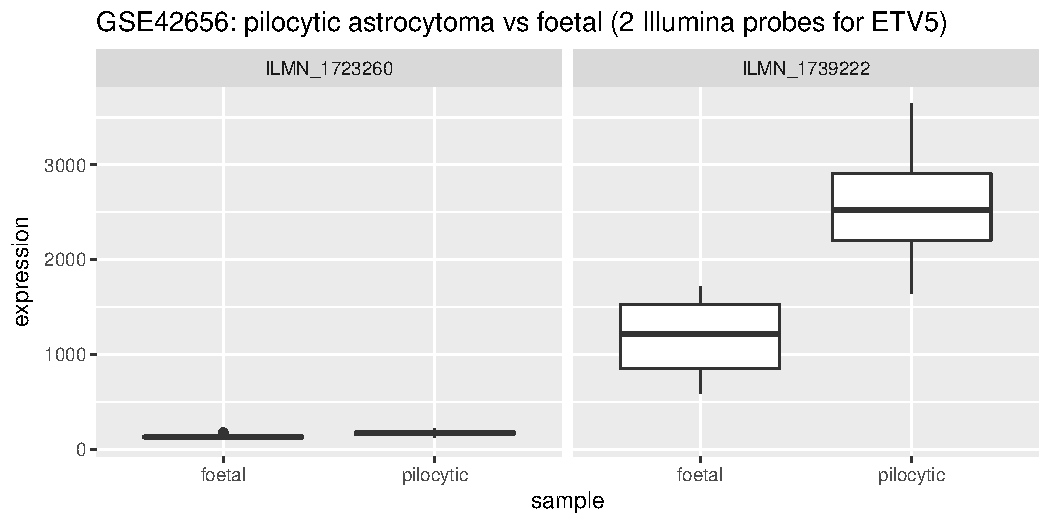
\includegraphics[width=\maxwidth]{figure/unnamed-chunk-23-1} 
\begin{kframe}\begin{alltt}
\hlkwd{ggplot}\hlstd{(ETV5_GSE42656_tidy,} \hlkwd{aes}\hlstd{(}\hlkwc{y}\hlstd{=expression,} \hlkwc{x}\hlstd{=sample2))} \hlopt{+}
  \hlkwd{geom_boxplot}\hlstd{()} \hlopt{+} \hlkwd{facet_grid}\hlstd{(.}\hlopt{~}\hlstd{ID_REF)} \hlopt{+}
  \hlkwd{ggtitle}\hlstd{(}\hlstr{"pilocytic astrocytoma vs foetal controls (Illumina probes for ETV5)"}\hlstd{)} \hlopt{+}
  \hlkwd{scale_y_continuous}\hlstd{(}\hlkwc{trans}\hlstd{=}\hlkwd{log2_trans}\hlstd{())} \hlopt{+} \hlkwd{xlab}\hlstd{(}\hlstr{""}\hlstd{)}
\end{alltt}
\end{kframe}
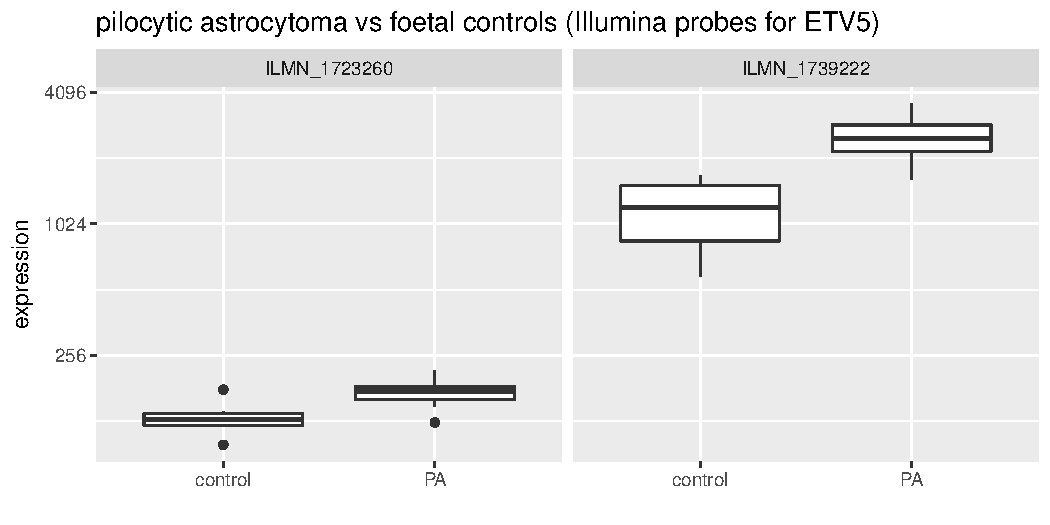
\includegraphics[width=\maxwidth]{figure/unnamed-chunk-23-2} 
\begin{kframe}\begin{alltt}
\hlcom{# ETV5_GSE12907 }
\hlstd{ETV5_GSE12907_t} \hlkwb{<-} \hlstd{GSE12907} \hlopt
  \hlkwd{left_join}\hlstd{(AffyIDs,} \hlkwc{by} \hlstd{=} \hlkwd{c}\hlstd{(}\hlstr{"ID_REF"} \hlstd{=} \hlstr{"PROBEID"}\hlstd{))} \hlopt
  \hlstd{dplyr}\hlopt{::}\hlkwd{select}\hlstd{(}\hlopt{-}\hlstd{ENTREZID,} \hlopt{-}\hlstd{GENENAME)}

\hlstd{all_p_12907} \hlkwb{<-} \hlkwd{as.numeric}\hlstd{()}
\hlkwa{for}\hlstd{(i} \hlkwa{in} \hlnum{1}\hlopt{:}\hlkwd{nrow}\hlstd{(ETV5_GSE12907_t))\{}
   \hlstd{all_p_12907[i]} \hlkwb{<-} \hlkwd{t.test}\hlstd{(ETV5_GSE12907_t[i,}\hlnum{2}\hlopt{:}\hlnum{22}\hlstd{], ETV5_GSE12907_t[i,}\hlnum{23}\hlopt{:}\hlnum{26}\hlstd{])}\hlopt{$}\hlstd{p.value}
 \hlstd{\}}
\hlkwd{mean}\hlstd{(all_p_12907} \hlopt{<=} \hlnum{0.05}\hlstd{)}
\end{alltt}
\begin{verbatim}
## [1] 0.241
\end{verbatim}
\begin{alltt}
\hlkwd{length}\hlstd{(all_p_12907)}
\end{alltt}
\begin{verbatim}
## [1] 24433
\end{verbatim}
\begin{alltt}
\hlkwa{for}\hlstd{(i} \hlkwa{in} \hlnum{1}\hlopt{:}\hlkwd{nrow}\hlstd{(ETV5_GSE12907))\{}
\hlkwd{print}\hlstd{(}\hlkwd{t.test}\hlstd{(ETV5_GSE12907[i,}\hlnum{2}\hlopt{:}\hlnum{15}\hlstd{], ETV5_GSE12907[i,}\hlnum{23}\hlopt{:}\hlnum{26}\hlstd{]))}
\hlstd{\}}
\end{alltt}
\begin{verbatim}
## 
## 	Welch Two Sample t-test
## 
## data:  ETV5_GSE12907[i, 2:15] and ETV5_GSE12907[i, 23:26]
## t = 6, df = 6, p-value = 0.001
## alternative hypothesis: true difference in means is not equal to 0
## 95 percent confidence interval:
##  197 502
## sample estimates:
## mean of x mean of y 
##       641       291 
## 
## 
## 	Welch Two Sample t-test
## 
## data:  ETV5_GSE12907[i, 2:15] and ETV5_GSE12907[i, 23:26]
## t = 8, df = 7, p-value = 5e-05
## alternative hypothesis: true difference in means is not equal to 0
## 95 percent confidence interval:
##  490 870
## sample estimates:
## mean of x mean of y 
##      1127       447 
## 
## 
## 	Welch Two Sample t-test
## 
## data:  ETV5_GSE12907[i, 2:15] and ETV5_GSE12907[i, 23:26]
## t = 7, df = 10, p-value = 3e-05
## alternative hypothesis: true difference in means is not equal to 0
## 95 percent confidence interval:
##  157 310
## sample estimates:
## mean of x mean of y 
##       476       243
\end{verbatim}
\begin{alltt}
\hlstd{ETV5_GSE12907_tidy} \hlkwb{<-} \hlstd{ETV5_GSE12907_tidy} \hlopt
  \hlkwd{mutate}\hlstd{(}\hlkwc{sample2} \hlstd{=} \hlkwd{ifelse}\hlstd{(sample}\hlopt{==}\hlstr{"CBM"}\hlstd{,} \hlstr{"control"}\hlstd{,} \hlstr{"PA"}\hlstd{))}

\hlkwd{ggplot}\hlstd{(ETV5_GSE12907_tidy,} \hlkwd{aes}\hlstd{(}\hlkwc{y}\hlstd{=expression,} \hlkwc{x}\hlstd{=sample))} \hlopt{+}
  \hlkwd{geom_boxplot}\hlstd{()} \hlopt{+} \hlkwd{facet_grid}\hlstd{(.}\hlopt{~}\hlstd{ID_REF)} \hlopt{+}
  \hlkwd{ggtitle}\hlstd{(}\hlstr{"GSE12907: pilocytic astrocytoma vs healthy cerebellum (Affy probes for ETV5)"}\hlstd{)}
\end{alltt}
\end{kframe}
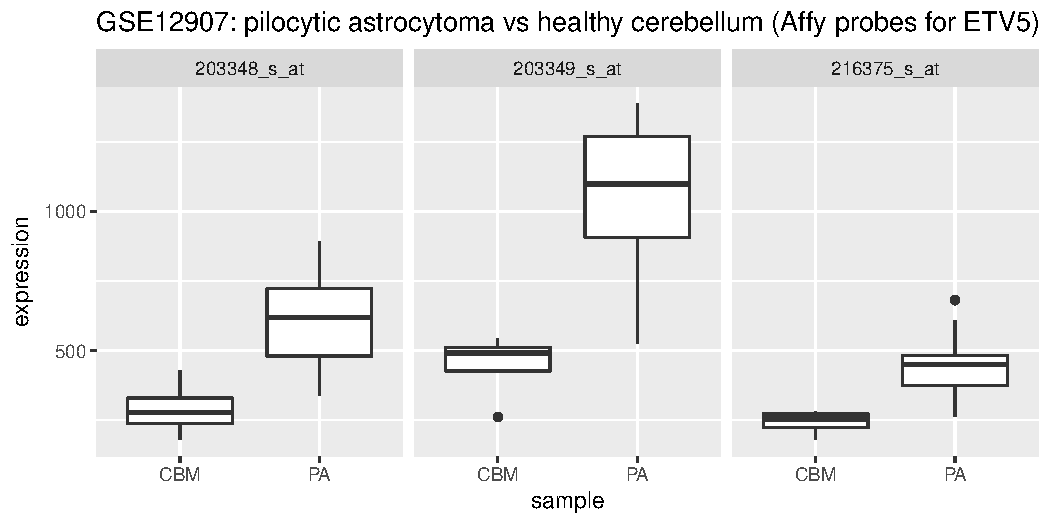
\includegraphics[width=\maxwidth]{figure/unnamed-chunk-23-3} 
\begin{kframe}\begin{alltt}
\hlkwd{ggplot}\hlstd{(ETV5_GSE12907_tidy,} \hlkwd{aes}\hlstd{(}\hlkwc{y}\hlstd{=expression,} \hlkwc{x}\hlstd{=sample))} \hlopt{+}
  \hlkwd{geom_boxplot}\hlstd{()} \hlopt{+} \hlkwd{facet_grid}\hlstd{(.}\hlopt{~}\hlstd{ID_REF)} \hlopt{+}
  \hlkwd{ggtitle}\hlstd{(}\hlstr{"GSE12907: pilocytic astrocytoma vs healthy cerebellum (Affy probes for ETV5)"}\hlstd{)} \hlopt{+}
  \hlkwd{scale_y_continuous}\hlstd{(}\hlkwc{trans}\hlstd{=}\hlkwd{log2_trans}\hlstd{())} \hlopt{+} \hlkwd{xlab}\hlstd{(}\hlstr{""}\hlstd{)}
\end{alltt}
\end{kframe}
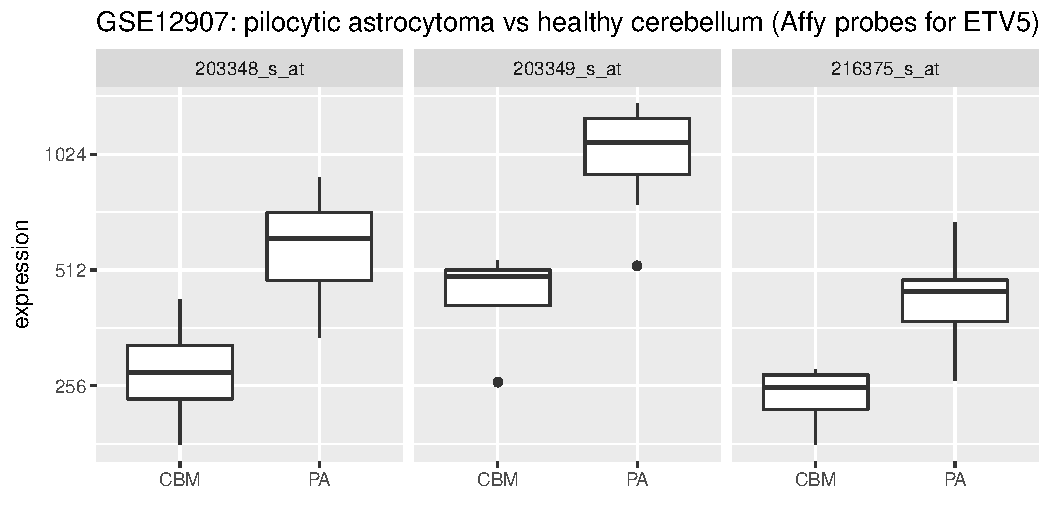
\includegraphics[width=\maxwidth]{figure/unnamed-chunk-23-4} 
\begin{kframe}\begin{alltt}
\hlstd{p1} \hlkwb{<-} \hlkwd{ggplot}\hlstd{(ETV5_GSE42656_tidy,} \hlkwd{aes}\hlstd{(}\hlkwc{y}\hlstd{=expression,} \hlkwc{x}\hlstd{=sample2))} \hlopt{+}
  \hlkwd{geom_boxplot}\hlstd{()} \hlopt{+} \hlkwd{facet_grid}\hlstd{(.}\hlopt{~}\hlstd{ID_REF)} \hlopt{+}
  \hlkwd{ggtitle}\hlstd{(}\hlstr{"PA vs foetal controls (Illumina probes for ETV5)"}\hlstd{)} \hlopt{+}
  \hlkwd{scale_y_continuous}\hlstd{(}\hlkwc{trans}\hlstd{=}\hlkwd{log2_trans}\hlstd{())} \hlopt{+} \hlkwd{xlab}\hlstd{(}\hlstr{""}\hlstd{)} \hlopt{+} \hlkwd{theme}\hlstd{(}\hlkwc{axis.text}\hlstd{=}\hlkwd{element_text}\hlstd{(}\hlkwc{size}\hlstd{=}\hlnum{16}\hlstd{))}
\hlstd{p2} \hlkwb{<-} \hlkwd{ggplot}\hlstd{(ETV5_GSE12907_tidy,} \hlkwd{aes}\hlstd{(}\hlkwc{y}\hlstd{=expression,} \hlkwc{x}\hlstd{=sample2))} \hlopt{+}
  \hlkwd{geom_boxplot}\hlstd{()} \hlopt{+} \hlkwd{facet_grid}\hlstd{(.}\hlopt{~}\hlstd{ID_REF)} \hlopt{+}
  \hlkwd{ggtitle}\hlstd{(}\hlstr{"PA vs healthy cerebellum (Affy probes for ETV5)"}\hlstd{)} \hlopt{+}
  \hlkwd{scale_y_continuous}\hlstd{(}\hlkwc{trans}\hlstd{=}\hlkwd{log2_trans}\hlstd{())} \hlopt{+} \hlkwd{xlab}\hlstd{(}\hlstr{""}\hlstd{)} \hlopt{+} \hlkwd{theme}\hlstd{(}\hlkwc{axis.text}\hlstd{=}\hlkwd{element_text}\hlstd{(}\hlkwc{size}\hlstd{=}\hlnum{16}\hlstd{))}
\hlkwd{multiplot}\hlstd{(p1,p2,}\hlkwc{cols}\hlstd{=}\hlnum{2}\hlstd{)}
\end{alltt}
\end{kframe}
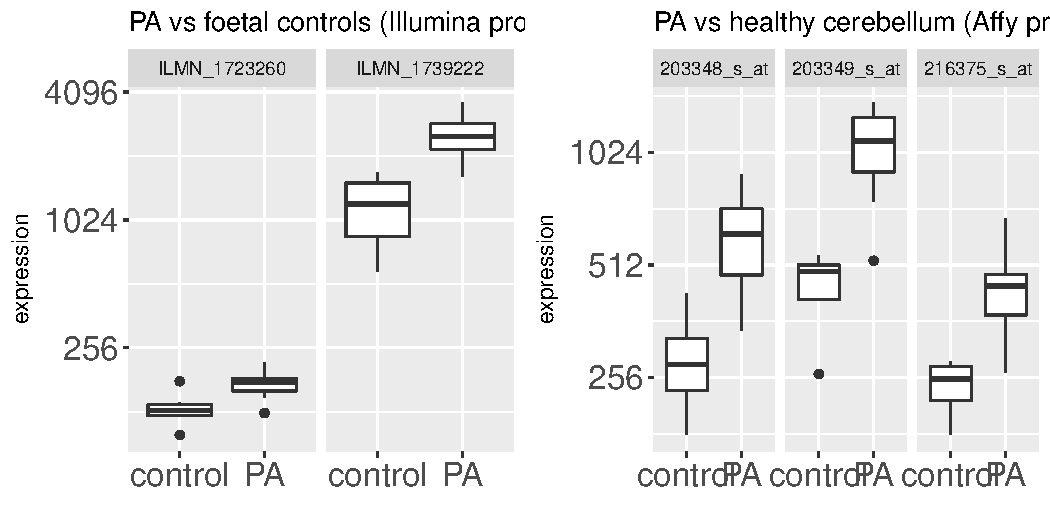
\includegraphics[width=\maxwidth]{figure/unnamed-chunk-23-5} 

\end{knitrout}


\subsection{t-tests on ETV5 {\it targets} for both datasets}

\subsubsection{GSE42656}

Using the 31 targets which were significant for the mouse data, we notice that the majority of the probes for those targets are significant using the human data as well.  Notice that 56.1\% of the 31 EVT5 target probes were significantly differentially expressed (not adjusted for multiple comparisons); 20/31 = 64.5\% of the ETV5 target genes were significantly differentially expressed.


Listed are the significant gene/probes (20 of 31 of the mouse-signifcant targets were also signficant in the GSE42656 dataset).  For example, SPRY4 is significant for two of the four probes.

\begin{knitrout}\small
\definecolor{shadecolor}{rgb}{0.969, 0.969, 0.969}\color{fgcolor}\begin{kframe}
\begin{alltt}
\hlstd{temp} \hlkwb{<-} \hlstd{tarGenesETV5[}\hlkwd{c}\hlstd{(tarGenesETV5}\hlopt{$}\hlstd{padj} \hlopt{<} \hlstd{siglevel} \hlopt{& !}\hlkwd{is.na}\hlstd{(tarGenesETV5}\hlopt{$}\hlstd{padj)),]}
\hlstd{ETV5_sig} \hlkwb{<-} \hlkwd{data.frame}\hlstd{(}\hlkwc{GENE}\hlstd{=}\hlkwd{as.character}\hlstd{(temp}\hlopt{$}\hlstd{GENE))}
\hlstd{ETV5_targets} \hlkwb{<-} \hlkwd{data.frame}\hlstd{(}\hlkwc{GENE}\hlstd{=}\hlkwd{as.character}\hlstd{(tarGenes}\hlopt{$}\hlstd{ETV5}\hlopt{$}\hlstd{GENE))}


\hlcom{# targets_GSE42656 - FOETAL}
\hlstd{targets_GSE42656} \hlkwb{<-} \hlstd{GSE42656} \hlopt
  \hlstd{dplyr}\hlopt{::}\hlkwd{select}\hlstd{(}\hlkwd{one_of}\hlstd{(}\hlkwd{c}\hlstd{(}\hlstr{"ID_REF"}\hlstd{, pilocytic, foetal)))} \hlopt
  \hlkwd{left_join}\hlstd{(IlluminaIDs,} \hlkwc{by} \hlstd{=} \hlkwd{c}\hlstd{(}\hlstr{"ID_REF"} \hlstd{=} \hlstr{"PROBEID"}\hlstd{))} \hlopt
  \hlstd{dplyr}\hlopt{::}\hlkwd{mutate}\hlstd{(}\hlkwc{SYMBOL} \hlstd{=} \hlkwd{toupper}\hlstd{(SYMBOL))} \hlopt
  \hlstd{dplyr}\hlopt{::}\hlkwd{filter}\hlstd{(SYMBOL} \hlopt \hlstd{ETV5_sig}\hlopt{$}\hlstd{GENE)} \hlopt
  \hlstd{dplyr}\hlopt{::}\hlkwd{select}\hlstd{(}\hlopt{-}\hlstd{ENTREZID,} \hlopt{-}\hlstd{GENENAME)} \hlopt
  \hlstd{dplyr}\hlopt{::}\hlkwd{filter}\hlstd{(}\hlopt{!}\hlkwd{is.na}\hlstd{(ID_REF))}


\hlstd{p_targ_GSE42656} \hlkwb{<-}\hlkwd{data.frame}\hlstd{(}\hlkwc{GENE}\hlstd{=}\hlkwd{character}\hlstd{(),} \hlkwc{PROBE}\hlstd{=}\hlkwd{character}\hlstd{(),}
                             \hlkwc{pvalue}\hlstd{=}\hlkwd{double}\hlstd{(),} \hlkwc{statistic}\hlstd{=}\hlkwd{double}\hlstd{())}

\hlkwa{for}\hlstd{(i} \hlkwa{in} \hlnum{1}\hlopt{:}\hlkwd{nrow}\hlstd{(targets_GSE42656))\{}
 \hlstd{temp} \hlkwb{<-} \hlkwd{t.test}\hlstd{(}\hlkwd{as.numeric}\hlstd{(targets_GSE42656[i,}\hlnum{2}\hlopt{:}\hlnum{15}\hlstd{]),}
                \hlkwd{as.numeric}\hlstd{(targets_GSE42656[i,}\hlnum{16}\hlopt{:}\hlnum{23}\hlstd{]))}
 \hlstd{temp2} \hlkwb{<-} \hlkwd{data.frame}\hlstd{(}\hlkwc{GENE} \hlstd{=} \hlkwd{as.character}\hlstd{(targets_GSE42656[i,}\hlnum{24}\hlstd{]),}
                     \hlkwc{PROBE} \hlstd{=} \hlkwd{as.character}\hlstd{(targets_GSE42656[i,}\hlnum{1}\hlstd{]),}
                     \hlkwc{pvalue} \hlstd{= temp}\hlopt{$}\hlstd{p.value,}
                     \hlkwc{statistic} \hlstd{= temp}\hlopt{$}\hlstd{statistic)}
 \hlstd{p_targ_GSE42656} \hlkwb{<-} \hlstd{p_targ_GSE42656} \hlopt \hlkwd{bind_rows}\hlstd{(temp2)}
\hlstd{\}}


\hlstd{p_targ_GSE42656} \hlopt
  \hlkwd{filter}\hlstd{(GENE} \hlopt \hlstd{ETV5_sig}\hlopt{$}\hlstd{GENE)} \hlopt
\hlcom{#  filter(pvalue <= 0.05) %>%}
\hlcom{#  summarize(n_distinct(GENE))}
  \hlkwd{summarize}\hlstd{(}\hlkwc{proportion.05} \hlstd{=} \hlkwd{mean}\hlstd{(pvalue} \hlopt{<=} \hlnum{0.05}\hlstd{))}
\end{alltt}
\begin{verbatim}
##   proportion.05
## 1         0.561
\end{verbatim}
\begin{alltt}
\hlstd{p_targ_GSE42656} \hlopt
  \hlkwd{filter}\hlstd{(GENE} \hlopt \hlstd{ETV5_sig}\hlopt{$}\hlstd{GENE)} \hlopt
  \hlkwd{ggplot}\hlstd{(}\hlkwd{aes}\hlstd{(}\hlkwc{x}\hlstd{=pvalue))} \hlopt{+} \hlkwd{geom_histogram}\hlstd{(}\hlkwc{binwidth} \hlstd{=} \hlnum{.05}\hlstd{)} \hlopt{+}
  \hlkwd{geom_vline}\hlstd{(}\hlkwc{xintercept} \hlstd{= siglevel)} \hlopt{+}
  \hlkwd{ggtitle}\hlstd{(}\hlstr{"GSE42656: All probes of the 31 targets significant in mouse data"}\hlstd{)}
\end{alltt}
\end{kframe}
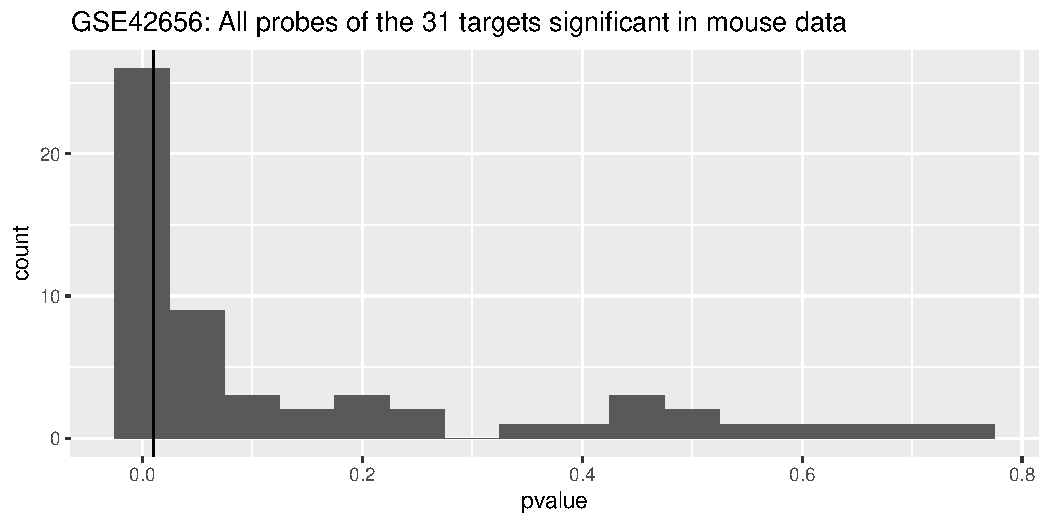
\includegraphics[width=\maxwidth]{figure/unnamed-chunk-24-1} 
\begin{kframe}\begin{alltt}
\hlcom{#siglevel/nrow(targets_GSE42656)  # no p-value adustment}
\hlstd{p_targ_GSE42656} \hlopt
  \hlkwd{filter}\hlstd{(GENE} \hlopt \hlstd{ETV5_sig}\hlopt{$}\hlstd{GENE)} \hlopt
  \hlkwd{filter}\hlstd{(pvalue} \hlopt{<=} \hlnum{0.05}\hlstd{)}  \hlopt
  \hlcom{#summarize(unique_genes = n_distinct(GENE))}
  \hlkwd{arrange}\hlstd{(pvalue)}
\end{alltt}
\begin{verbatim}
##       GENE        PROBE   pvalue statistic
## 1   SPRED1 ILMN_1804277 2.88e-11     15.03
## 2    SPRY4 ILMN_2086105 3.77e-09     11.41
## 3   KCNIP1 ILMN_1744387 1.00e-07      8.08
## 4    SPRY4 ILMN_1797596 5.42e-07      7.43
## 5     LRP4 ILMN_1675268 1.13e-06      8.02
## 6     NT5E ILMN_1697220 2.29e-06      7.30
## 7    DUSP6 ILMN_2396020 3.28e-06      6.63
## 8    NLGN3 ILMN_1759700 4.67e-06      6.85
## 9   ELOVL2 ILMN_1716843 7.82e-06     -8.11
## 10   TPPP3 ILMN_1797744 8.78e-06      6.28
## 11   DUSP6 ILMN_1677466 2.24e-05      5.74
## 12   SPRY2 ILMN_2089329 4.08e-05      5.24
## 13 PCDHGC3 ILMN_2274355 6.43e-05      5.34
## 14  SPATA6 ILMN_1775926 2.01e-04      5.01
## 15   SOCS2 ILMN_2131861 2.39e-04     -4.54
## 16 PCDHGC3 ILMN_1656955 2.94e-04      4.38
## 17   SOCS2 ILMN_1798926 3.89e-04     -4.38
## 18 PCDHGC3 ILMN_2251963 7.52e-04      3.97
## 19  KCNIP1 ILMN_2368856 8.26e-04      3.94
## 20   FABP7 ILMN_1745299 9.22e-04     -3.90
## 21 PCDHGC3 ILMN_2251961 1.13e-03      3.84
## 22 PCDHGC3 ILMN_2345824 1.53e-03      3.67
## 23 PCDHGC3 ILMN_1675428 4.07e-03      3.44
## 24  RSBN1L ILMN_1712027 6.20e-03     -3.19
## 25     AK4 ILMN_1798249 7.84e-03     -3.52
## 26    GLDC ILMN_1806754 8.09e-03      2.95
## 27   BTBD3 ILMN_1713964 2.94e-02     -2.72
## 28    SHC3 ILMN_1770905 3.45e-02      2.39
## 29   S1PR1 ILMN_1653504 3.45e-02     -2.46
## 30     AK4 ILMN_1843198 3.46e-02     -2.50
## 31     AK4 ILMN_1764090 3.71e-02     -2.34
## 32     AK4 ILMN_2338038 4.21e-02     -2.41
\end{verbatim}
\begin{alltt}
\hlstd{p_targ_GSE42656} \hlopt
  \hlkwd{filter}\hlstd{(GENE} \hlopt \hlstd{ETV5_sig}\hlopt{$}\hlstd{GENE)} \hlopt
  \hlkwd{filter}\hlstd{(pvalue} \hlopt{<=} \hlnum{0.05}\hlstd{)}  \hlopt
  \hlkwd{summarize}\hlstd{(}\hlkwc{unique_genes} \hlstd{=} \hlkwd{n_distinct}\hlstd{(GENE))}
\end{alltt}
\begin{verbatim}
##   unique_genes
## 1           20
\end{verbatim}
\begin{alltt}
\hlstd{targets_GSE42656_tidy} \hlkwb{<-} \hlstd{targets_GSE42656} \hlopt
  \hlstd{tidyr}\hlopt{::}\hlkwd{gather}\hlstd{(sampleID, expression,} \hlopt{-}\hlkwd{c}\hlstd{(ID_REF,SYMBOL))} \hlopt
  \hlkwd{mutate}\hlstd{(}\hlkwc{expression} \hlstd{=} \hlkwd{parse_number}\hlstd{(expression))} \hlopt
  \hlkwd{mutate}\hlstd{(}\hlkwc{sample} \hlstd{=} \hlkwd{ifelse}\hlstd{(sampleID} \hlopt \hlstd{pilocytic,} \hlstr{"pilocytic"}\hlstd{,} \hlstr{"foetal"}\hlstd{))}


\hlstd{genename} \hlkwb{<-} \hlkwd{data.frame}\hlstd{(}\hlkwc{GENE}\hlstd{=}\hlstr{"SPRY4"}\hlstd{)}
\hlstd{onegene_GSE42656} \hlkwb{<-} \hlstd{GSE42656} \hlopt
  \hlstd{dplyr}\hlopt{::}\hlkwd{select}\hlstd{(}\hlkwd{one_of}\hlstd{(}\hlkwd{c}\hlstd{(}\hlstr{"ID_REF"}\hlstd{, pilocytic, foetal)))} \hlopt
  \hlkwd{left_join}\hlstd{(IlluminaIDs,} \hlkwc{by} \hlstd{=} \hlkwd{c}\hlstd{(}\hlstr{"ID_REF"} \hlstd{=} \hlstr{"PROBEID"}\hlstd{))} \hlopt
  \hlkwd{mutate}\hlstd{(}\hlkwc{SYMBOL} \hlstd{=} \hlkwd{toupper}\hlstd{(SYMBOL))} \hlopt
  \hlkwd{right_join}\hlstd{(genename,} \hlkwc{by}\hlstd{=}\hlkwd{c}\hlstd{(}\hlstr{"SYMBOL"}\hlstd{=} \hlstr{"GENE"}\hlstd{))} \hlopt
  \hlstd{dplyr}\hlopt{::}\hlkwd{select}\hlstd{(}\hlopt{-}\hlstd{ENTREZID,} \hlopt{-}\hlstd{GENENAME)}

\hlkwa{for}\hlstd{(i} \hlkwa{in} \hlnum{1}\hlopt{:}\hlkwd{nrow}\hlstd{(onegene_GSE42656))\{}
  \hlkwd{print}\hlstd{(}\hlkwd{t.test}\hlstd{(onegene_GSE42656[i,}\hlnum{2}\hlopt{:}\hlnum{15}\hlstd{], onegene_GSE42656[i,}\hlnum{16}\hlopt{:}\hlnum{23}\hlstd{]))}
\hlstd{\}}
\end{alltt}
\begin{verbatim}
## 
## 	Welch Two Sample t-test
## 
## data:  onegene_GSE42656[i, 2:15] and onegene_GSE42656[i, 16:23]
## t = 1, df = 20, p-value = 0.2
## alternative hypothesis: true difference in means is not equal to 0
## 95 percent confidence interval:
##  -1.83  9.49
## sample estimates:
## mean of x mean of y 
##       132       128 
## 
## 
## 	Welch Two Sample t-test
## 
## data:  onegene_GSE42656[i, 2:15] and onegene_GSE42656[i, 16:23]
## t = -0.5, df = 20, p-value = 0.6
## alternative hypothesis: true difference in means is not equal to 0
## 95 percent confidence interval:
##  -6.66  3.90
## sample estimates:
## mean of x mean of y 
##       112       114 
## 
## 
## 	Welch Two Sample t-test
## 
## data:  onegene_GSE42656[i, 2:15] and onegene_GSE42656[i, 16:23]
## t = 7, df = 20, p-value = 5e-07
## alternative hypothesis: true difference in means is not equal to 0
## 95 percent confidence interval:
##  31.0 55.3
## sample estimates:
## mean of x mean of y 
##       167       124 
## 
## 
## 	Welch Two Sample t-test
## 
## data:  onegene_GSE42656[i, 2:15] and onegene_GSE42656[i, 16:23]
## t = 10, df = 20, p-value = 4e-09
## alternative hypothesis: true difference in means is not equal to 0
## 95 percent confidence interval:
##   987 1437
## sample estimates:
## mean of x mean of y 
##      1619       407
\end{verbatim}
\begin{alltt}
\hlstd{targets_GSE42656_tidy} \hlopt
  \hlkwd{filter}\hlstd{(SYMBOL} \hlopt \hlstd{genename)} \hlopt
  \hlkwd{ggplot}\hlstd{(}\hlkwd{aes}\hlstd{(}\hlkwc{y}\hlstd{=expression,} \hlkwc{x}\hlstd{=sample))} \hlopt{+}
  \hlkwd{geom_boxplot}\hlstd{()} \hlopt{+} \hlkwd{facet_grid}\hlstd{(.}\hlopt{~}\hlstd{ID_REF)} \hlopt{+}
  \hlkwd{ggtitle}\hlstd{(}\hlkwd{paste}\hlstd{(}\hlstr{"GSE42656, Gene:"}\hlstd{,genename))}
\end{alltt}
\end{kframe}
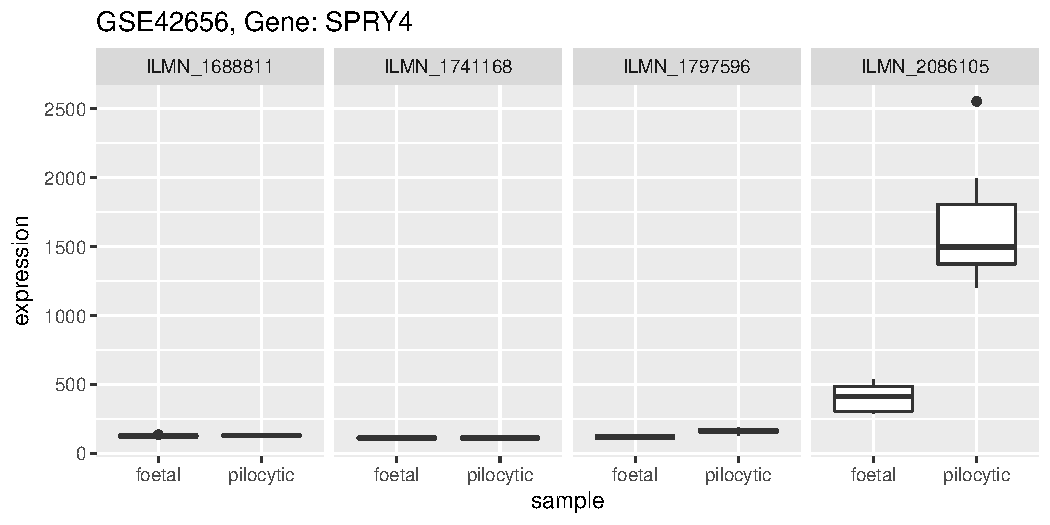
\includegraphics[width=\maxwidth]{figure/unnamed-chunk-24-2} 

\end{knitrout}

\subsubsection{GSE12907}

Using the 31 targets which were significant for the mouse data, we notice that the majority of the probes for those targets are significant using the human data as well.  Notice that 40.8\% of the 31 EVT5 target probes (49 probes) were significantly differentially expressed (not adjusted for multiple comparisons); 12/31 = 38.7\% of the ETV5 target genes were significantly differentially expressed.


Listed are the significant gene/probes (12 of 31 of the mouse-signifcant targets were also signficant in the human dataset).  

\begin{knitrout}\small
\definecolor{shadecolor}{rgb}{0.969, 0.969, 0.969}\color{fgcolor}\begin{kframe}
\begin{alltt}
\hlcom{# targets_GSE12907}
\hlstd{targets_GSE12907} \hlkwb{<-} \hlstd{GSE12907} \hlopt
  \hlstd{dplyr}\hlopt{::}\hlkwd{select}\hlstd{(}\hlkwd{one_of}\hlstd{(}\hlkwd{c}\hlstd{(}\hlstr{"ID_REF"}\hlstd{, pilocytic12907, CBM)))} \hlopt
  \hlkwd{left_join}\hlstd{(AffyIDs,} \hlkwc{by} \hlstd{=} \hlkwd{c}\hlstd{(}\hlstr{"ID_REF"} \hlstd{=} \hlstr{"PROBEID"}\hlstd{))} \hlopt
  \hlkwd{mutate}\hlstd{(}\hlkwc{SYMBOL} \hlstd{=} \hlkwd{toupper}\hlstd{(SYMBOL))} \hlopt
  \hlkwd{filter}\hlstd{(SYMBOL} \hlopt \hlstd{ETV5_targets}\hlopt{$}\hlstd{GENE)} \hlopt
  \hlstd{dplyr}\hlopt{::}\hlkwd{select}\hlstd{(}\hlopt{-}\hlstd{ENTREZID,} \hlopt{-}\hlstd{GENENAME)} \hlopt
  \hlkwd{filter}\hlstd{(}\hlopt{!}\hlkwd{is.na}\hlstd{(ID_REF))}

\hlstd{p_targ_GSE12907} \hlkwb{<-}\hlkwd{data.frame}\hlstd{(}\hlkwc{GENE}\hlstd{=}\hlkwd{character}\hlstd{(),} \hlkwc{PROBE}\hlstd{=}\hlkwd{character}\hlstd{(),}
                             \hlkwc{pvalue}\hlstd{=}\hlkwd{double}\hlstd{(),} \hlkwc{statistic}\hlstd{=}\hlkwd{double}\hlstd{())}

\hlkwa{for}\hlstd{(i} \hlkwa{in} \hlnum{1}\hlopt{:}\hlkwd{nrow}\hlstd{(targets_GSE12907))\{}
 \hlstd{temp} \hlkwb{<-} \hlkwd{t.test}\hlstd{(targets_GSE12907[i,}\hlnum{2}\hlopt{:}\hlnum{22}\hlstd{], targets_GSE12907[i,}\hlnum{23}\hlopt{:}\hlnum{26}\hlstd{])}
 \hlstd{temp2} \hlkwb{<-} \hlkwd{data.frame}\hlstd{(}\hlkwc{GENE} \hlstd{=} \hlkwd{as.character}\hlstd{(targets_GSE12907[i,}\hlnum{27}\hlstd{]),}
                     \hlkwc{PROBE} \hlstd{=} \hlkwd{as.character}\hlstd{(targets_GSE12907[i,}\hlnum{1}\hlstd{]),}
                     \hlkwc{pvalue} \hlstd{= temp}\hlopt{$}\hlstd{p.value,}
                     \hlkwc{statistic} \hlstd{= temp}\hlopt{$}\hlstd{statistic)}
 \hlstd{p_targ_GSE12907} \hlkwb{<-} \hlstd{p_targ_GSE12907} \hlopt \hlkwd{bind_rows}\hlstd{(temp2)}
\hlstd{\}}


\hlstd{p_targ_GSE12907} \hlopt
  \hlkwd{filter}\hlstd{(GENE} \hlopt \hlstd{ETV5_sig}\hlopt{$}\hlstd{GENE)} \hlopt
  \hlkwd{summarize}\hlstd{(}\hlkwc{proportion.05} \hlstd{=} \hlkwd{mean}\hlstd{(pvalue} \hlopt{<=} \hlnum{0.05}\hlstd{))}
\end{alltt}
\begin{verbatim}
##   proportion.05
## 1         0.408
\end{verbatim}
\begin{alltt}
\hlcom{#siglevel/nrow(targets_GSE12907)  # no p-value adustment}
\hlstd{p_targ_GSE12907} \hlopt
  \hlkwd{filter}\hlstd{(GENE} \hlopt \hlstd{ETV5_sig}\hlopt{$}\hlstd{GENE)} \hlopt
  \hlkwd{filter}\hlstd{(pvalue} \hlopt{<=} \hlnum{0.05}\hlstd{)}  \hlopt
  \hlkwd{arrange}\hlstd{(pvalue)}
\end{alltt}
\begin{verbatim}
##        GENE       PROBE   pvalue statistic
## 1     DUSP6   208891_at 1.01e-10     11.60
## 2     NLGN3   219726_at 1.58e-10     10.98
## 3     DUSP6 208893_s_at 5.93e-10     10.22
## 4    SPATA6 220298_s_at 8.02e-09     10.19
## 5     DUSP6 208892_s_at 2.19e-08      9.01
## 6    SPATA6   220299_at 5.27e-08      9.40
## 7      NT5E   203939_at 1.09e-07      9.70
## 8     SPRY4 221489_s_at 3.06e-07      8.66
## 9      LRP4 212850_s_at 1.21e-05      7.83
## 10   KCNIP1   221307_at 1.76e-05      5.60
## 11  PCDHGC3 211066_x_at 1.07e-04     10.44
## 12  PCDHGC3 215836_s_at 1.34e-04     10.46
## 13  PCDHGC3 214564_s_at 1.83e-04      4.45
## 14  PCDHGC3 205717_x_at 2.16e-04      9.83
## 15  PCDHGC3 209079_x_at 2.30e-04     10.06
## 16  PCDHGC3 211876_x_at 3.08e-03      3.47
## 17     SHC3 206330_s_at 7.89e-03      4.29
## 18    FABP5 202345_s_at 1.21e-02      3.29
## 19 SLC9A3R1   201349_at 2.13e-02     -3.64
## 20   ELOVL2   213712_at 4.49e-02     -2.93
\end{verbatim}
\begin{alltt}
\hlstd{p_targ_GSE12907} \hlopt
  \hlkwd{filter}\hlstd{(GENE} \hlopt \hlstd{ETV5_sig}\hlopt{$}\hlstd{GENE)} \hlopt
  \hlkwd{filter}\hlstd{(pvalue} \hlopt{<=} \hlnum{0.05}\hlstd{)}  \hlopt
  \hlkwd{summarize}\hlstd{(}\hlkwc{unique_genes} \hlstd{=} \hlkwd{n_distinct}\hlstd{(GENE))}
\end{alltt}
\begin{verbatim}
##   unique_genes
## 1           12
\end{verbatim}
\begin{alltt}
\hlstd{p_targ_GSE12907} \hlopt
  \hlkwd{filter}\hlstd{(GENE} \hlopt \hlstd{ETV5_sig}\hlopt{$}\hlstd{GENE)} \hlopt
  \hlkwd{ggplot}\hlstd{(}\hlkwd{aes}\hlstd{(}\hlkwc{x}\hlstd{=pvalue))} \hlopt{+} \hlkwd{geom_histogram}\hlstd{(}\hlkwc{binwidth} \hlstd{=} \hlnum{.05}\hlstd{)} \hlopt{+}
  \hlkwd{geom_vline}\hlstd{(}\hlkwc{xintercept} \hlstd{= siglevel)} \hlopt{+}
  \hlkwd{ggtitle}\hlstd{(}\hlstr{"GSE12907: All probes of the 31 targets significant in mouse data"}\hlstd{)}
\end{alltt}
\end{kframe}
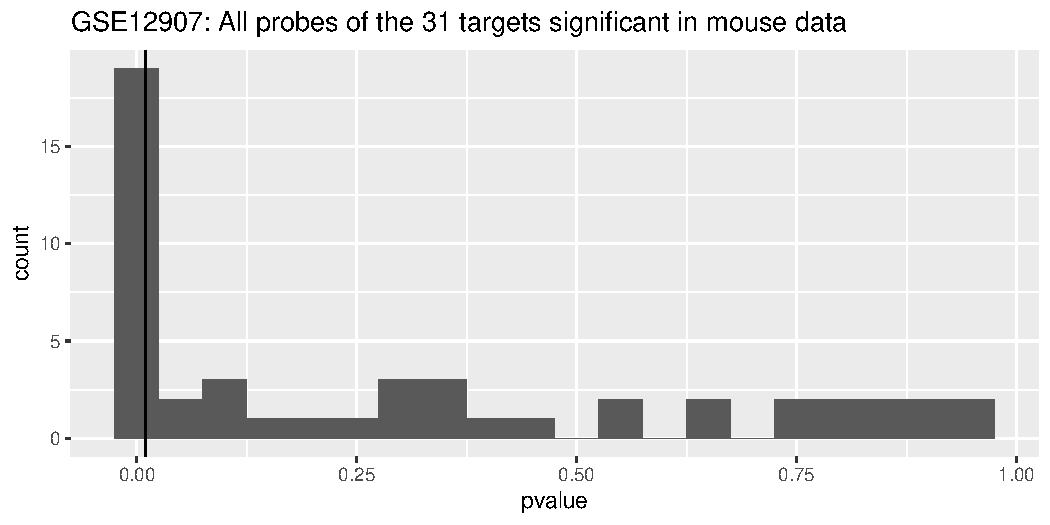
\includegraphics[width=\maxwidth]{figure/unnamed-chunk-25-1} 

\end{knitrout}

\subsubsection{Comparing directionality of DE changes}
\begin{knitrout}\small
\definecolor{shadecolor}{rgb}{0.969, 0.969, 0.969}\color{fgcolor}\begin{kframe}
\begin{alltt}
\hlstd{tarGenes31} \hlkwb{<-} \hlkwd{lapply}\hlstd{(tarGenesP,}
                     \hlkwa{function}\hlstd{(}\hlkwc{x}\hlstd{) x[}\hlkwd{c}\hlstd{(x}\hlopt{$}\hlstd{padj} \hlopt{<} \hlstd{siglevel} \hlopt{& !}\hlkwd{is.na}\hlstd{(x}\hlopt{$}\hlstd{padj)),])}\hlopt{$}\hlstd{ETV} \hlopt
  \hlkwd{arrange}\hlstd{(padj)}

\hlstd{p_sig31_GSE12907} \hlkwb{<-} \hlstd{p_targ_GSE12907} \hlopt
  \hlkwd{filter}\hlstd{(GENE} \hlopt \hlstd{ETV5_sig}\hlopt{$}\hlstd{GENE)} \hlopt
  \hlkwd{filter}\hlstd{(pvalue} \hlopt{<=}\hlnum{0.05}\hlstd{)}

\hlstd{p_targ_GSE42656} \hlopt
  \hlkwd{filter}\hlstd{(GENE} \hlopt \hlstd{ETV5_sig}\hlopt{$}\hlstd{GENE)} \hlopt
  \hlkwd{filter}\hlstd{(pvalue} \hlopt{<=} \hlnum{0.05}\hlstd{)}  \hlopt
  \hlkwd{full_join}\hlstd{(p_sig31_GSE12907,} \hlkwc{by}\hlstd{=}\hlstr{"GENE"}\hlstd{)} \hlopt
  \hlkwd{full_join}\hlstd{(tarGenes31,} \hlkwc{by}\hlstd{=}\hlstr{"GENE"}\hlstd{)} \hlopt
  \hlkwd{mutate}\hlstd{(}\hlkwc{changemouse} \hlstd{=} \hlkwd{ifelse}\hlstd{(log2FoldChange} \hlopt{>} \hlnum{0}\hlstd{,} \hlstr{"up"}\hlstd{,} \hlstr{"down"}\hlstd{))} \hlopt
  \hlkwd{mutate}\hlstd{(}\hlkwc{change42656} \hlstd{=} \hlkwd{ifelse}\hlstd{(statistic.x} \hlopt{>} \hlnum{0}\hlstd{,} \hlstr{"up"}\hlstd{,} \hlstr{"down"}\hlstd{))} \hlopt
  \hlkwd{mutate}\hlstd{(}\hlkwc{change12907} \hlstd{=} \hlkwd{ifelse}\hlstd{(statistic.y} \hlopt{>} \hlnum{0}\hlstd{,} \hlstr{"up"}\hlstd{,} \hlstr{"down"}\hlstd{))} \hlopt
  \hlkwd{mutate}\hlstd{(}\hlkwc{pmouse} \hlstd{= padj,} \hlkwc{p42656} \hlstd{= pvalue.x,} \hlkwc{p12907} \hlstd{= pvalue.y)} \hlopt
  \hlstd{dplyr}\hlopt{::}\hlkwd{select}\hlstd{(GENE, changemouse, pmouse,change12907, p12907, change42656, p42656)} \hlopt
  \hlkwd{arrange}\hlstd{(GENE)}
\end{alltt}
\begin{verbatim}
##        GENE changemouse   pmouse change12907   p12907 change42656   p42656
## 1       AK4          up 2.77e-03        <NA>       NA        down 3.71e-02
## 2       AK4          up 2.77e-03        <NA>       NA        down 7.84e-03
## 3       AK4          up 2.77e-03        <NA>       NA        down 3.46e-02
## 4       AK4          up 2.77e-03        <NA>       NA        down 4.21e-02
## 5     BTBD3          up 1.62e-06        <NA>       NA        down 2.94e-02
## 6     CHST2          up 1.26e-08        <NA>       NA        <NA>       NA
## 7    COL2A1          up 4.43e-03        <NA>       NA        <NA>       NA
## 8    CXCL14          up 7.29e-14        <NA>       NA        <NA>       NA
## 9    DNAJB4        down 1.65e-03        <NA>       NA        <NA>       NA
## 10    DOCK4          up 1.73e-03        <NA>       NA        <NA>       NA
## 11    DUSP6          up 5.54e-03          up 1.01e-10          up 2.24e-05
## 12    DUSP6          up 5.54e-03          up 2.19e-08          up 2.24e-05
## 13    DUSP6          up 5.54e-03          up 5.93e-10          up 2.24e-05
## 14    DUSP6          up 5.54e-03          up 1.01e-10          up 3.28e-06
## 15    DUSP6          up 5.54e-03          up 2.19e-08          up 3.28e-06
## 16    DUSP6          up 5.54e-03          up 5.93e-10          up 3.28e-06
## 17   ELOVL2          up 9.28e-09        down 4.49e-02        down 7.82e-06
## 18    FABP5          up 3.93e-07          up 1.21e-02        <NA>       NA
## 19    FABP7          up 3.02e-03        <NA>       NA        down 9.22e-04
## 20    GAP43        down 1.27e-03        <NA>       NA        <NA>       NA
## 21     GJA1          up 1.26e-07        <NA>       NA        <NA>       NA
## 22     GLDC          up 5.29e-04        <NA>       NA          up 8.09e-03
## 23   IGFBP6        down 9.10e-03        <NA>       NA        <NA>       NA
## 24   KCNIP1        down 9.09e-03          up 1.76e-05          up 1.00e-07
## 25   KCNIP1        down 9.09e-03          up 1.76e-05          up 8.26e-04
## 26     LRP4          up 2.77e-03          up 1.21e-05          up 1.13e-06
## 27    MMP15          up 7.07e-03        <NA>       NA        <NA>       NA
## 28    NLGN3          up 1.21e-03          up 1.58e-10          up 4.67e-06
## 29     NT5E        down 4.76e-03          up 1.09e-07          up 2.29e-06
## 30  PCDHGC3          up 2.09e-04          up 2.16e-04          up 2.94e-04
## 31  PCDHGC3          up 2.09e-04          up 2.30e-04          up 2.94e-04
## 32  PCDHGC3          up 2.09e-04          up 1.07e-04          up 2.94e-04
## 33  PCDHGC3          up 2.09e-04          up 3.08e-03          up 2.94e-04
## 34  PCDHGC3          up 2.09e-04          up 1.83e-04          up 2.94e-04
## 35  PCDHGC3          up 2.09e-04          up 1.34e-04          up 2.94e-04
## 36  PCDHGC3          up 2.09e-04          up 2.16e-04          up 4.07e-03
## 37  PCDHGC3          up 2.09e-04          up 2.30e-04          up 4.07e-03
## 38  PCDHGC3          up 2.09e-04          up 1.07e-04          up 4.07e-03
## 39  PCDHGC3          up 2.09e-04          up 3.08e-03          up 4.07e-03
## 40  PCDHGC3          up 2.09e-04          up 1.83e-04          up 4.07e-03
## 41  PCDHGC3          up 2.09e-04          up 1.34e-04          up 4.07e-03
## 42  PCDHGC3          up 2.09e-04          up 2.16e-04          up 1.13e-03
## 43  PCDHGC3          up 2.09e-04          up 2.30e-04          up 1.13e-03
## 44  PCDHGC3          up 2.09e-04          up 1.07e-04          up 1.13e-03
## 45  PCDHGC3          up 2.09e-04          up 3.08e-03          up 1.13e-03
## 46  PCDHGC3          up 2.09e-04          up 1.83e-04          up 1.13e-03
## 47  PCDHGC3          up 2.09e-04          up 1.34e-04          up 1.13e-03
## 48  PCDHGC3          up 2.09e-04          up 2.16e-04          up 7.52e-04
## 49  PCDHGC3          up 2.09e-04          up 2.30e-04          up 7.52e-04
## 50  PCDHGC3          up 2.09e-04          up 1.07e-04          up 7.52e-04
## 51  PCDHGC3          up 2.09e-04          up 3.08e-03          up 7.52e-04
## 52  PCDHGC3          up 2.09e-04          up 1.83e-04          up 7.52e-04
## 53  PCDHGC3          up 2.09e-04          up 1.34e-04          up 7.52e-04
## 54  PCDHGC3          up 2.09e-04          up 2.16e-04          up 6.43e-05
## 55  PCDHGC3          up 2.09e-04          up 2.30e-04          up 6.43e-05
## 56  PCDHGC3          up 2.09e-04          up 1.07e-04          up 6.43e-05
## 57  PCDHGC3          up 2.09e-04          up 3.08e-03          up 6.43e-05
## 58  PCDHGC3          up 2.09e-04          up 1.83e-04          up 6.43e-05
## 59  PCDHGC3          up 2.09e-04          up 1.34e-04          up 6.43e-05
## 60  PCDHGC3          up 2.09e-04          up 2.16e-04          up 1.53e-03
## 61  PCDHGC3          up 2.09e-04          up 2.30e-04          up 1.53e-03
## 62  PCDHGC3          up 2.09e-04          up 1.07e-04          up 1.53e-03
## 63  PCDHGC3          up 2.09e-04          up 3.08e-03          up 1.53e-03
## 64  PCDHGC3          up 2.09e-04          up 1.83e-04          up 1.53e-03
## 65  PCDHGC3          up 2.09e-04          up 1.34e-04          up 1.53e-03
## 66   RSBN1L        down 7.15e-03        <NA>       NA        down 6.20e-03
## 67    S1PR1          up 9.28e-14        <NA>       NA        down 3.45e-02
## 68     SHC3          up 8.35e-03          up 7.89e-03          up 3.45e-02
## 69 SLC9A3R1          up 1.51e-04        down 2.13e-02        <NA>       NA
## 70    SOCS2        down 6.28e-03        <NA>       NA        down 3.89e-04
## 71    SOCS2        down 6.28e-03        <NA>       NA        down 2.39e-04
## 72   SPATA6        down 5.86e-03          up 8.02e-09          up 2.01e-04
## 73   SPATA6        down 5.86e-03          up 5.27e-08          up 2.01e-04
## 74   SPRED1          up 7.78e-04        <NA>       NA          up 2.88e-11
## 75    SPRY2          up 2.41e-06        <NA>       NA          up 4.08e-05
## 76    SPRY4          up 2.87e-03          up 3.06e-07          up 5.42e-07
## 77    SPRY4          up 2.87e-03          up 3.06e-07          up 3.77e-09
## 78    TPPP3        down 2.94e-03        <NA>       NA          up 8.78e-06
\end{verbatim}
\begin{alltt}
\hlstd{best_targets} \hlkwb{<-} \hlstd{p_targ_GSE42656} \hlopt
  \hlkwd{filter}\hlstd{(GENE} \hlopt \hlstd{ETV5_sig}\hlopt{$}\hlstd{GENE)} \hlopt
  \hlkwd{filter}\hlstd{(pvalue} \hlopt{<=} \hlnum{0.05}\hlstd{)}  \hlopt
  \hlkwd{full_join}\hlstd{(p_sig31_GSE12907,} \hlkwc{by}\hlstd{=}\hlstr{"GENE"}\hlstd{)} \hlopt
  \hlkwd{full_join}\hlstd{(tarGenes31,} \hlkwc{by}\hlstd{=}\hlstr{"GENE"}\hlstd{)} \hlopt
  \hlkwd{mutate}\hlstd{(}\hlkwc{changemouse} \hlstd{=} \hlkwd{ifelse}\hlstd{(log2FoldChange} \hlopt{>} \hlnum{0}\hlstd{,} \hlstr{"up"}\hlstd{,} \hlstr{"down"}\hlstd{))} \hlopt
  \hlkwd{mutate}\hlstd{(}\hlkwc{change42656} \hlstd{=} \hlkwd{ifelse}\hlstd{(statistic.x} \hlopt{>} \hlnum{0}\hlstd{,} \hlstr{"up"}\hlstd{,} \hlstr{"down"}\hlstd{))} \hlopt
  \hlkwd{mutate}\hlstd{(}\hlkwc{change12907} \hlstd{=} \hlkwd{ifelse}\hlstd{(statistic.y} \hlopt{>} \hlnum{0}\hlstd{,} \hlstr{"up"}\hlstd{,} \hlstr{"down"}\hlstd{))} \hlopt
  \hlkwd{mutate}\hlstd{(}\hlkwc{pmouse} \hlstd{= padj,} \hlkwc{p42656} \hlstd{= pvalue.x,} \hlkwc{p12907} \hlstd{= pvalue.y)} \hlopt
  \hlstd{dplyr}\hlopt{::}\hlkwd{select}\hlstd{(GENE, changemouse, change12907, change42656)} \hlopt
  \hlkwd{filter}\hlstd{(changemouse} \hlopt{==} \hlstd{change12907} \hlopt{|} \hlstd{changemouse} \hlopt{==} \hlstd{change42656)} \hlopt
  \hlkwd{distinct}\hlstd{()} \hlopt
  \hlkwd{arrange}\hlstd{(GENE)}


\hlstd{best_targets}
\end{alltt}
\begin{verbatim}
##       GENE changemouse change12907 change42656
## 1    DUSP6          up          up          up
## 2    FABP5          up          up        <NA>
## 3     GLDC          up        <NA>          up
## 4     LRP4          up          up          up
## 5    NLGN3          up          up          up
## 6  PCDHGC3          up          up          up
## 7   RSBN1L        down        <NA>        down
## 8     SHC3          up          up          up
## 9    SOCS2        down        <NA>        down
## 10  SPRED1          up        <NA>          up
## 11   SPRY2          up        <NA>          up
## 12   SPRY4          up          up          up
\end{verbatim}
\begin{alltt}
\hlkwd{xtable}\hlstd{(best_targets)}
\end{alltt}
\begin{verbatim}
## % latex table generated in R 3.4.2 by xtable 1.8-2 package
## % Tue Jan 23 05:14:29 2018
## \begin{table}[ht]
## \centering
## \begin{tabular}{rllll}
##   \hline
##  & GENE & changemouse & change12907 & change42656 \\ 
##   \hline
## 1 & DUSP6 & up & up & up \\ 
##   2 & FABP5 & up & up &  \\ 
##   3 & GLDC & up &  & up \\ 
##   4 & LRP4 & up & up & up \\ 
##   5 & NLGN3 & up & up & up \\ 
##   6 & PCDHGC3 & up & up & up \\ 
##   7 & RSBN1L & down &  & down \\ 
##   8 & SHC3 & up & up & up \\ 
##   9 & SOCS2 & down &  & down \\ 
##   10 & SPRED1 & up &  & up \\ 
##   11 & SPRY2 & up &  & up \\ 
##   12 & SPRY4 & up & up & up \\ 
##    \hline
## \end{tabular}
## \end{table}
\end{verbatim}
\end{kframe}
\end{knitrout}

\subsubsection{Note:}

To confirm that the data human datasets were appropriate to use in comparison to the mouse data, we did a few analyses.  We first checked that the data were normalized, indeed, quantile normalization was used with GSE42656.  Additionally, to scale the differential expression, we looked at the global differential expression rates.  In GSE42656, of all the probes, approximately 1/3 were differentially expressed;  of the probes associated with the 31 signficant ETV5 target genes, more than half were differentially expressed in the human data.  In GSE12907, of all the probes, approximately 24\% were differentially expressed;  of the probes associated with the 31 signficant ETV5 target genes, 41\% were differentially expressed.

\subsection{GO Analysis, GSE42656 only}

Below are the top categories for the 31 targets which are differentially expressed.  The category ``negative regulation of response to stimulus''  is over-represented in our 31 genes (with 12 of 31 being involved in the category).


\begin{knitrout}\small
\definecolor{shadecolor}{rgb}{0.969, 0.969, 0.969}\color{fgcolor}\begin{kframe}
\begin{alltt}
\hlstd{assayed.genes} \hlkwb{<-} \hlstd{DEanalysis}\hlopt{$}\hlstd{gene}
\hlstd{de.genes} \hlkwb{<-} \hlstd{ETV5_sig}\hlopt{$}\hlstd{GENE}
\hlstd{target.genes} \hlkwb{<-} \hlstd{ETV5_targets}\hlopt{$}\hlstd{GENE}

\hlstd{gene.vector}\hlkwb{=}\hlkwd{as.integer}\hlstd{(assayed.genes}\hlopt\hlstd{de.genes)}
\hlkwd{names}\hlstd{(gene.vector)}\hlkwb{=}\hlstd{assayed.genes}

\hlstd{de.pwf} \hlkwb{=} \hlkwd{nullp}\hlstd{(gene.vector,} \hlkwc{genome}\hlstd{=}\hlstr{'mm9'}\hlstd{,} \hlkwc{id}\hlstd{=}\hlstr{'geneSymbol'}\hlstd{,} \hlkwc{plot.fit}\hlstd{=}\hlnum{FALSE}\hlstd{)}  \hlcom{#prob weighting function}

\hlstd{gopvals} \hlkwb{=} \hlkwd{goseq}\hlstd{(de.pwf,} \hlkwc{genome}\hlstd{=}\hlstr{'mm9'}\hlstd{,} \hlkwc{id}\hlstd{=}\hlstr{'geneSymbol'}\hlstd{,} \hlkwc{test.cats}\hlstd{=}\hlkwd{c}\hlstd{(}\hlstr{"GO:BP"}\hlstd{))}
\hlstd{gopvals[}\hlkwd{p.adjust}\hlstd{(gopvals}\hlopt{$}\hlstd{over_represented_pvalue,} \hlkwc{method} \hlstd{=} \hlstr{"BH"}\hlstd{)} \hlopt{<} \hlnum{0.05}\hlstd{,]}
\end{alltt}
\begin{verbatim}
##         category over_represented_pvalue under_represented_pvalue
## 8283  GO:0048585                7.96e-07                        1
## 6901  GO:0043407                3.60e-06                        1
## 10455 GO:0070373                4.22e-06                        1
## 6903  GO:0043409                4.79e-06                        1
##       numDEInCat numInCat                                         term
## 8283          12     1382  negative regulation of response to stimulus
## 6901           4       65   negative regulation of MAP kinase activity
## 10455          4       66 negative regulation of ERK1 and ERK2 cascade
## 6903           5      152          negative regulation of MAPK cascade
##       ontology
## 8283        BP
## 6901        BP
## 10455       BP
## 6903        BP
\end{verbatim}
\begin{alltt}
\hlkwd{xtable}\hlstd{(gopvals[}\hlkwd{p.adjust}\hlstd{(gopvals}\hlopt{$}\hlstd{over_represented_pvalue,} \hlkwc{method} \hlstd{=} \hlstr{"BH"}\hlstd{)} \hlopt{<} \hlnum{0.05}\hlstd{,}\hlkwd{c}\hlstd{(}\hlnum{1}\hlstd{,}\hlnum{6}\hlstd{)])}
\end{alltt}
\begin{verbatim}
## % latex table generated in R 3.4.2 by xtable 1.8-2 package
## % Tue Jan 23 05:14:43 2018
## \begin{table}[ht]
## \centering
## \begin{tabular}{rll}
##   \hline
##  & category & term \\ 
##   \hline
## 8283 & GO:0048585 & negative regulation of response to stimulus \\ 
##   6901 & GO:0043407 & negative regulation of MAP kinase activity \\ 
##   10455 & GO:0070373 & negative regulation of ERK1 and ERK2 cascade \\ 
##   6903 & GO:0043409 & negative regulation of MAPK cascade \\ 
##    \hline
## \end{tabular}
## \end{table}
\end{verbatim}
\begin{alltt}
\hlstd{enriched.GO} \hlkwb{=} \hlstd{gopvals}\hlopt{$}\hlstd{category[}\hlkwd{p.adjust}\hlstd{(gopvals}\hlopt{$}\hlstd{over_represented_pvalue,} \hlkwc{method} \hlstd{=} \hlstr{"BH"}\hlstd{)} \hlopt{<} \hlnum{0.05}\hlstd{]}

\hlcom{## To find what the GO categories are:  }
\hlkwa{for} \hlstd{(go} \hlkwa{in} \hlstd{enriched.GO)\{}
  \hlkwd{print}\hlstd{(GOTERM[[go]])}
  \hlkwd{cat}\hlstd{(}\hlstr{"----------------------------------------------\textbackslash{}n"}\hlstd{)}
  \hlstd{\}}
\end{alltt}
\begin{verbatim}
## GOID: GO:0048585
## Term: negative regulation of response to stimulus
## Ontology: BP
## Definition: Any process that stops, prevents, or reduces the
##     frequency, rate or extent of a response to a stimulus.
##     Response to stimulus is a change in state or activity of a
##     cell or an organism (in terms of movement, secretion, enzyme
##     production, gene expression, etc.) as a result of a stimulus.
## Synonym: down regulation of response to stimulus
## Synonym: down-regulation of response to stimulus
## Synonym: downregulation of response to stimulus
## Synonym: inhibition of response to stimulus
## ----------------------------------------------
## GOID: GO:0043407
## Term: negative regulation of MAP kinase activity
## Ontology: BP
## Definition: Any process that stops, prevents, or reduces the
##     frequency, rate or extent of MAP kinase activity.
## Synonym: down regulation of MAPK activity
## Synonym: down-regulation of MAPK activity
## Synonym: downregulation of MAPK activity
## Synonym: inhibition of MAPK activity
## Synonym: negative regulation of mitogen activated protein kinase
##     activity
## Synonym: negative regulation of mitogen-activated protein kinase
##     activity
## ----------------------------------------------
## GOID: GO:0070373
## Term: negative regulation of ERK1 and ERK2 cascade
## Ontology: BP
## Definition: Any process that stops, prevents, or reduces the
##     frequency, rate or extent of signal transduction mediated by
##     the ERK1 and ERK2 cascade.
## Synonym: down regulation of ERK1 and ERK2 cascade
## Synonym: down-regulation of ERK1 and ERK2 cascade
## Synonym: downregulation of ERK1 and ERK2 cascade
## Synonym: inhibition of ERK1 and ERK2 cascade
## Synonym: negative regulation of ERK cascade
## Synonym: negative regulation of ERK1 and ERK2 signaling pathway
## Synonym: negative regulation of ERK1 and ERK2 signalling pathway
## Synonym: negative regulation of ERK1 cascade
## Synonym: negative regulation of ERK1/2 cascade
## Synonym: negative regulation of ERK2 cascade
## Synonym: negative regulation of MAPK1 cascade
## Synonym: negative regulation of MAPK3 cascade
## ----------------------------------------------
## GOID: GO:0043409
## Term: negative regulation of MAPK cascade
## Ontology: BP
## Definition: Any process that stops, prevents, or reduces the
##     frequency, rate or extent of signal transduction mediated by
##     the MAPKKK cascade.
## Synonym: down regulation of MAPK cascade
## Synonym: down regulation of MAPKKK cascade
## Synonym: down-regulation of MAPK cascade
## Synonym: down-regulation of MAPKKK cascade
## Synonym: downregulation of MAPK cascade
## Synonym: downregulation of MAPKKK cascade
## Synonym: inhibition of MAPK cascade
## Synonym: inhibition of MAPKKK cascade
## Synonym: negative regulation of MAP kinase cascade
## Synonym: negative regulation of MAP kinase kinase kinase cascade
## Synonym: negative regulation of MAPKKK cascade
## Synonym: negative regulation of mitogen activated protein kinase
##     cascade
## Synonym: negative regulation of mitogen activated protein kinase
##     kinase kinase cascade
## Synonym: negative regulation of mitogen-activated protein kinase
##     cascade
## Synonym: negative regulation of mitogen-activated protein kinase
##     kinase kinase cascade
## ----------------------------------------------
\end{verbatim}
\end{kframe}
\end{knitrout}



%%%%%%%%%%%%%%%%%%%%%%%%%%%%%%%%%%%%%%%%%%%%%%%%%%%%%%%%%%%%%%%%%%%%%%%%%%%%%
%%%%%%%%%%%%%%%%%%%%%%%%%%%%%%%%%%%%%%%%%%%%%%%%%%%%%%%%%%%%%%%%%%%%%%%%%%%%%
%%%%%%%%%%%%%%%%%%%%%%%%%%%%%%%%%%%%%%%%%%%%%%%%%%%%%%%%%%%%%%%%%%%%%%%%%%%%%
%%%%%%%%%%%%%%%%%%%%%%%%%%%%%%%%%%%%%%%%%%%%%%%%%%%%%%%%%%%%%%%%%%%%%%%%%%%%%

\newpage
\section{New Mouse Data}

On November 22, 2016, Peter Sims gave us additional data.  The additional data consist of three 6-week FF and three 6-week FMC mouse optic nerve RNA-seq samples.  We will use the observations to identify if ETV5 is still significant and also to see if the same targets are differentially expressed (and in what direction).

\subsection{Normalizing and DE for young data}

\begin{knitrout}\small
\definecolor{shadecolor}{rgb}{0.969, 0.969, 0.969}\color{fgcolor}\begin{kframe}
\begin{alltt}
\hlstd{micefinalyoung} \hlkwb{<-} \hlkwd{read.delim}\hlstd{(}\hlstr{"FF6wks_FMC6wks.cts.txt"}\hlstd{)}
\hlkwd{colnames}\hlstd{(micefinalyoung)} \hlkwb{<-} \hlkwd{c}\hlstd{(}\hlstr{"gene"}\hlstd{,} \hlkwd{paste}\hlstd{(}\hlstr{"FFY"}\hlstd{,} \hlnum{1}\hlopt{:}\hlnum{3}\hlstd{,} \hlkwc{sep}\hlstd{=}\hlstr{""}\hlstd{),}
                              \hlkwd{paste}\hlstd{(}\hlstr{"FMCY"}\hlstd{,} \hlnum{1}\hlopt{:}\hlnum{3}\hlstd{,} \hlkwc{sep}\hlstd{=}\hlstr{""}\hlstd{))}

\hlstd{geneinfo} \hlkwb{<-} \hlkwd{read_excel}\hlstd{(}\hlstr{"FF_FMC_matrixv2.xlsx"}\hlstd{,}
                       \hlkwc{col_names}\hlstd{=}\hlkwd{c}\hlstd{(}\hlstr{"gene"}\hlstd{,} \hlstr{"REFSEQ_ID"}\hlstd{,} \hlkwd{paste}\hlstd{(}\hlstr{"FF"}\hlstd{,} \hlnum{1}\hlopt{:}\hlnum{5}\hlstd{,} \hlkwc{sep}\hlstd{=}\hlstr{""}\hlstd{),}
                                   \hlkwd{paste}\hlstd{(}\hlstr{"FMC"}\hlstd{,}\hlnum{1}\hlopt{:}\hlnum{5}\hlstd{,} \hlkwc{sep}\hlstd{=}\hlstr{""}\hlstd{),} \hlstr{"X"}\hlstd{,} \hlkwd{paste}\hlstd{(}\hlstr{"FFk"}\hlstd{,}\hlnum{1}\hlopt{:}\hlnum{5}\hlstd{,}\hlkwc{sep}\hlstd{=}\hlstr{""}\hlstd{),}
                                   \hlkwd{paste}\hlstd{(}\hlstr{"FMCk"}\hlstd{,}\hlnum{1}\hlopt{:}\hlnum{5}\hlstd{,}\hlkwc{sep}\hlstd{=}\hlstr{""}\hlstd{)))}
\hlstd{geneinfo} \hlkwb{<-} \hlstd{geneinfo} \hlopt \hlstd{dplyr}\hlopt{::}\hlkwd{select}\hlstd{(gene, REFSEQ_ID)}

\hlstd{micefinalyoung} \hlkwb{<-} \hlstd{micefinalyoung} \hlopt \hlkwd{left_join}\hlstd{(geneinfo,} \hlkwc{by}\hlstd{=}\hlstr{"gene"}\hlstd{)}

\hlstd{condyoung} \hlkwb{<-} \hlkwd{factor}\hlstd{(}\hlkwd{c}\hlstd{(}\hlkwd{rep}\hlstd{(}\hlstr{"FFY"}\hlstd{,} \hlnum{3}\hlstd{),} \hlkwd{rep}\hlstd{(}\hlstr{"FMCY"}\hlstd{,} \hlnum{3}\hlstd{)))}
\hlstd{ddsyoung} \hlkwb{<-} \hlstd{DESeq2}\hlopt{::}\hlkwd{DESeqDataSetFromMatrix}\hlstd{(micefinalyoung[,}\hlopt{-}\hlkwd{c}\hlstd{(}\hlnum{1}\hlstd{,}\hlnum{8}\hlstd{)],}
                                           \hlkwd{DataFrame}\hlstd{(condyoung),} \hlopt{~} \hlstd{condyoung)}
\hlstd{ddsyoung} \hlkwb{<-} \hlstd{DESeq2}\hlopt{::}\hlkwd{DESeq}\hlstd{(ddsyoung)}
\hlstd{resyoung} \hlkwb{<-} \hlkwd{results}\hlstd{(ddsyoung)}  \hlcom{# Diff Exp results if we want/need the p-values}
\hlstd{dds.datayoung} \hlkwb{<-} \hlkwd{counts}\hlstd{(ddsyoung,} \hlkwc{normalized}\hlstd{=}\hlnum{TRUE}\hlstd{)}
\hlstd{miceoutyoung} \hlkwb{<-} \hlkwd{data.frame}\hlstd{(}\hlkwc{gene}\hlstd{=}\hlkwd{toupper}\hlstd{(micefinalyoung}\hlopt{$}\hlstd{gene),}
                           \hlkwc{REFSEQ_ID}\hlstd{=micefinalyoung}\hlopt{$}\hlstd{REFSEQ_ID, dds.datayoung)}
\hlstd{micepsyoung} \hlkwb{<-} \hlkwd{data.frame}\hlstd{(}\hlkwc{gene}\hlstd{=}\hlkwd{toupper}\hlstd{(micefinalyoung}\hlopt{$}\hlstd{gene),}
                          \hlkwc{REFSEQ_ID}\hlstd{=micefinalyoung}\hlopt{$}\hlstd{REFSEQ_ID, resyoung)}
\end{alltt}
\end{kframe}
\end{knitrout}

\subsection{Significance of ETV5 and its targets}

\begin{knitrout}\small
\definecolor{shadecolor}{rgb}{0.969, 0.969, 0.969}\color{fgcolor}\begin{kframe}
\begin{alltt}
\hlcom{# the 504 target genes of ETV5 with the ORIGINAL DE p-values}
\hlstd{ETV5andtargets} \hlkwb{<-} \hlkwd{data.frame}\hlstd{(}\hlkwc{GENE} \hlstd{=} \hlkwd{c}\hlstd{(}\hlstr{"ETV5"}\hlstd{, tarGenesETV5[,}\hlnum{1}\hlstd{]))}
\hlkwd{head}\hlstd{(tarGenesETV5)}
\end{alltt}
\begin{verbatim}
##          GENE pvalue  padj log2FoldChange
## 1        ABI1 0.3099 0.565         0.1080
## 2      KHDC1L     NA    NA             NA
## 3 ZSCAN16-AS1     NA    NA             NA
## 4     BCL2L11 0.8686 0.943        -0.0344
## 5       ABCB6 0.8503 0.934        -0.0401
## 6       TSSC4 0.0513 0.211         0.4401
\end{verbatim}
\begin{alltt}
\hlcom{# now investigating the new p-values with the 6-week mice data}
\hlstd{DEpsyoung} \hlkwb{=} \hlstd{micepsyoung[,}\hlkwd{c}\hlstd{(}\hlstr{"gene"}\hlstd{,} \hlstr{"pvalue"}\hlstd{,} \hlstr{"padj"}\hlstd{,} \hlstr{"log2FoldChange"}\hlstd{)]}
\hlstd{DEpsyoung} \hlkwb{=} \hlstd{DEpsyoung} \hlopt \hlkwd{mutate}\hlstd{(}\hlkwc{GENE}\hlstd{=gene)} \hlopt \hlstd{dplyr}\hlopt{::}\hlkwd{select}\hlstd{(}\hlopt{-}\hlstd{gene)}

\hlstd{micefinalyoung} \hlopt \hlkwd{filter}\hlstd{(gene} \hlopt{==} \hlstr{"Etv5"}\hlstd{)} \hlcom{# raw data}
\end{alltt}
\begin{verbatim}
##   gene FFY1 FFY2 FFY3 FMCY1 FMCY2 FMCY3 REFSEQ_ID
## 1 Etv5  223  172  152   332   260   249 NM_023794
\end{verbatim}
\begin{alltt}
\hlstd{miceoutyoung} \hlopt \hlkwd{filter}\hlstd{(gene} \hlopt{==} \hlstr{"ETV5"}\hlstd{)} \hlcom{# normalized data}
\end{alltt}
\begin{verbatim}
##   gene REFSEQ_ID FFY1 FFY2 FFY3 FMCY1 FMCY2 FMCY3
## 1 ETV5 NM_023794  239  154  171   285   262   262
\end{verbatim}
\begin{alltt}
\hlstd{DEpsyoung} \hlopt \hlkwd{filter}\hlstd{(GENE} \hlopt{==} \hlstr{"ETV5"}\hlstd{)} \hlcom{# DE results}
\end{alltt}
\begin{verbatim}
##   pvalue  padj log2FoldChange GENE
## 1 0.0113 0.298          0.523 ETV5
\end{verbatim}
\begin{alltt}
\hlstd{norm6wkdata} \hlkwb{<-} \hlstd{miceoutyoung} \hlopt \hlkwd{filter}\hlstd{(gene} \hlopt{==} \hlstr{"ETV5"}\hlstd{)} \hlopt \hlstd{dplyr}\hlopt{::}\hlkwd{select}\hlstd{(}\hlkwd{starts_with}\hlstd{(}\hlstr{"F"}\hlstd{))}

\hlstd{normdataplot} \hlkwb{<-} \hlkwd{data.frame}\hlstd{(}\hlkwc{data6wk} \hlstd{=} \hlkwd{unlist}\hlstd{(norm6wkdata),} \hlkwc{sample}\hlstd{=}\hlkwd{c}\hlstd{(}\hlkwd{rep}\hlstd{(}\hlstr{"FFY"}\hlstd{,}\hlnum{3}\hlstd{),} \hlkwd{rep}\hlstd{(}\hlstr{"FMCY"}\hlstd{,}\hlnum{3}\hlstd{)))}

\hlstd{normdataplot} \hlkwb{<-} \hlstd{normdataplot} \hlopt
  \hlkwd{mutate}\hlstd{(}\hlkwc{sample2} \hlstd{=} \hlkwd{ifelse}\hlstd{(sample} \hlopt{==} \hlstr{"FFY"}\hlstd{,} \hlstr{"control optic nerve"}\hlstd{,} \hlstr{"optic glioma-bearing nerve"}\hlstd{))} \hlopt
  \hlkwd{mutate}\hlstd{(}\hlkwc{labelpos} \hlstd{=} \hlkwd{ifelse}\hlstd{(normdataplot}\hlopt{$}\hlstd{sample}\hlopt{==}\hlstr{'FMCY'}\hlstd{,}
                          \hlkwd{ifelse}\hlstd{(normdataplot}\hlopt{$}\hlstd{data6wk} \hlopt{<} \hlnum{262.2}\hlstd{,} \hlopt{-}\hlnum{2}\hlstd{,} \hlkwd{ifelse}\hlstd{(normdataplot}\hlopt{$}\hlstd{data6wk} \hlopt{<} \hlnum{265}\hlstd{,} \hlnum{2}\hlstd{,} \hlnum{0}\hlstd{)),}\hlnum{0}\hlstd{))}

\hlkwd{ggplot}\hlstd{(normdataplot,} \hlkwd{aes}\hlstd{(}\hlkwc{x}\hlstd{=sample2,} \hlkwc{y}\hlstd{=}\hlkwd{as.numeric}\hlstd{(data6wk),}
                         \hlkwc{label}\hlstd{=}\hlkwd{round}\hlstd{(}\hlkwd{as.numeric}\hlstd{(data6wk),}\hlnum{2}\hlstd{),} \hlkwc{shape}\hlstd{=sample2))} \hlopt{+}
       \hlkwd{ylab}\hlstd{(}\hlstr{"normalized expression count"}\hlstd{)} \hlopt{+}
       \hlkwd{xlab}\hlstd{(}\hlstr{""}\hlstd{)} \hlopt{+} \hlkwd{theme}\hlstd{(}\hlkwc{axis.text}\hlstd{=}\hlkwd{element_text}\hlstd{(}\hlkwc{size}\hlstd{=}\hlnum{16}\hlstd{))} \hlopt{+}
       \hlkwd{geom_point}\hlstd{(}\hlkwc{size}\hlstd{=}\hlnum{10}\hlstd{)}  \hlopt{+} \hlkwd{theme}\hlstd{(}\hlkwc{legend.position}\hlstd{=}\hlstr{"none"}\hlstd{)} \hlopt{+}
  \hlkwd{scale_shape_manual}\hlstd{(}\hlkwc{values}\hlstd{=}\hlkwd{c}\hlstd{(}\hlnum{10}\hlstd{,}\hlnum{12}\hlstd{))}\hlopt{+}
  \hlkwd{geom_text}\hlstd{(}\hlkwc{nudge_y}\hlstd{=normdataplot}\hlopt{$}\hlstd{labelpos,} \hlkwc{nudge_x}\hlstd{=}\hlnum{0.15}\hlstd{,} \hlkwc{size}\hlstd{=}\hlnum{6}\hlstd{)} \hlopt{+}
  \hlkwd{ggtitle}\hlstd{(}\hlstr{"ETV5 expression in 6-week old mice"}\hlstd{)}
\end{alltt}
\end{kframe}
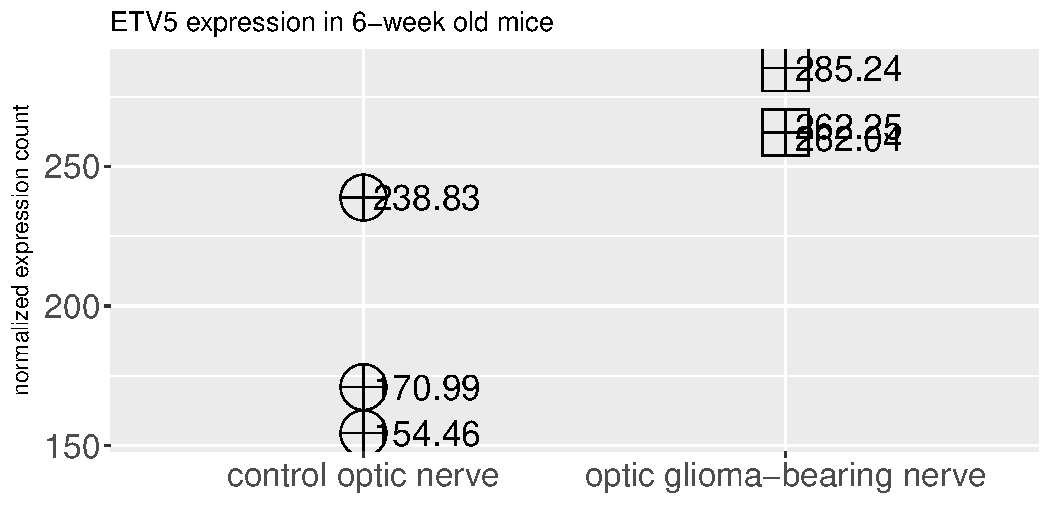
\includegraphics[width=\maxwidth]{figure/unnamed-chunk-29-1} 
\begin{kframe}\begin{alltt}
\hlcom{# the first 10 of all 504 targets of ETV5}
\hlkwd{left_join}\hlstd{(ETV5andtargets, DEpsyoung,} \hlkwc{by}\hlstd{=} \hlstr{"GENE"}\hlstd{)} \hlopt
  \hlkwd{arrange}\hlstd{(padj)} \hlopt
  \hlkwd{head}\hlstd{(}\hlnum{10}\hlstd{)}
\end{alltt}
\begin{verbatim}
##        GENE   pvalue     padj log2FoldChange
## 1     FABP7 2.31e-16 8.40e-13          1.245
## 2     FABP5 1.19e-12 1.32e-09          1.208
## 3  SLC39A12 1.29e-07 3.58e-05          0.693
## 4    ELOVL2 2.44e-07 5.79e-05          2.047
## 5    SPRED1 1.41e-05 1.91e-03          0.555
## 6     S1PR1 1.76e-05 2.25e-03          0.739
## 7    LHFPL3 3.68e-05 4.07e-03          0.778
## 8   FAM181B 4.59e-05 4.85e-03          1.349
## 9     CHST2 4.84e-05 5.08e-03          0.655
## 10    ACSL3 8.56e-05 7.89e-03          0.547
\end{verbatim}
\begin{alltt}
\hlcom{# the 31 targets which were DE in the original data}
\hlkwd{left_join}\hlstd{(ETV5andtargets, DEpsyoung,} \hlkwc{by}\hlstd{=} \hlstr{"GENE"}\hlstd{)} \hlopt
  \hlkwd{filter}\hlstd{(GENE} \hlopt \hlstd{ETV5_sig}\hlopt{$}\hlstd{GENE)} \hlopt
  \hlkwd{arrange}\hlstd{(padj)}
\end{alltt}
\begin{verbatim}
##        GENE   pvalue     padj log2FoldChange
## 1     FABP7 2.31e-16 8.40e-13        1.24487
## 2     FABP5 1.19e-12 1.32e-09        1.20821
## 3    ELOVL2 2.44e-07 5.79e-05        2.04672
## 4    SPRED1 1.41e-05 1.91e-03        0.55473
## 5     S1PR1 1.76e-05 2.25e-03        0.73925
## 6     CHST2 4.84e-05 5.08e-03        0.65504
## 7   PCDHGC3 8.94e-05 8.14e-03        0.58749
## 8      GJA1 5.60e-04 3.76e-02        0.59708
## 9      LRP4 7.34e-04 4.72e-02        0.64095
## 10    MMP15 1.28e-03 7.19e-02        0.57434
## 11    SPRY4 1.42e-02 3.47e-01        0.70673
## 12 SLC9A3R1 1.60e-02 3.74e-01        0.37267
## 13   CXCL14 2.20e-02 4.43e-01        0.53143
## 14    SOCS2 3.31e-02 5.47e-01       -0.69123
## 15    SPRY2 4.04e-02 5.96e-01        0.54697
## 16    TPPP3 6.76e-02 7.26e-01       -0.33613
## 17     GLDC 8.45e-02 7.87e-01        0.62879
## 18    BTBD3 1.49e-01 9.39e-01        0.33526
## 19   DNAJB4 9.94e-01 1.00e+00       -0.00113
## 20   COL2A1 2.06e-01 1.00e+00        0.44377
## 21    DUSP6 9.92e-01 1.00e+00        0.00201
## 22      AK4 2.74e-01 1.00e+00        0.27608
## 23   RSBN1L 4.84e-01 1.00e+00        0.10420
## 24    GAP43 6.74e-01 1.00e+00       -0.08051
## 25   KCNIP1 9.09e-01 1.00e+00        0.04114
## 26   IGFBP6 9.16e-01 1.00e+00        0.02516
## 27     NT5E 8.93e-01 1.00e+00        0.02881
## 28     SHC3 2.41e-01 1.00e+00        0.34651
## 29    NLGN3 3.23e-01 1.00e+00        0.19639
## 30   SPATA6 6.31e-01 1.00e+00       -0.13586
## 31    DOCK4 2.81e-01 1.00e+00        0.20033
\end{verbatim}
\begin{alltt}
\hlkwd{left_join}\hlstd{(ETV5andtargets, DEpsyoung,} \hlkwc{by}\hlstd{=} \hlstr{"GENE"}\hlstd{)} \hlopt
  \hlkwd{filter}\hlstd{(GENE} \hlopt \hlstd{ETV5_sig}\hlopt{$}\hlstd{GENE)} \hlopt
  \hlkwd{arrange}\hlstd{(padj)} \hlopt
  \hlkwd{ggplot}\hlstd{(}\hlkwd{aes}\hlstd{(}\hlkwc{x}\hlstd{=pvalue))} \hlopt{+}
  \hlkwd{geom_histogram}\hlstd{(}\hlkwc{binwidth}\hlstd{=}\hlnum{0.05}\hlstd{)} \hlopt{+}
  \hlkwd{geom_vline}\hlstd{(}\hlkwc{xintercept}\hlstd{=siglevel)} \hlopt{+}
  \hlkwd{ggtitle}\hlstd{(}\hlstr{"6 week mouse data: All 31 targets significant in mouse data"}\hlstd{)}
\end{alltt}
\end{kframe}
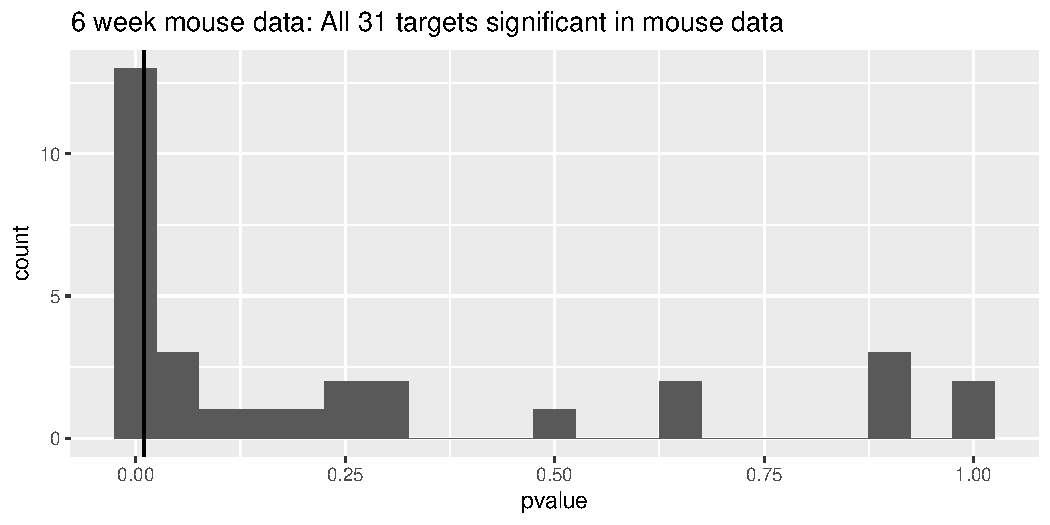
\includegraphics[width=\maxwidth]{figure/unnamed-chunk-29-2} 

\end{knitrout}

\subsubsection{Adding the young data to up/down comparison}

\begin{knitrout}\small
\definecolor{shadecolor}{rgb}{0.969, 0.969, 0.969}\color{fgcolor}\begin{kframe}
\begin{alltt}
\hlstd{best_targets} \hlkwb{<-} \hlstd{p_targ_GSE42656} \hlopt
  \hlkwd{filter}\hlstd{(GENE} \hlopt \hlstd{ETV5_sig}\hlopt{$}\hlstd{GENE)} \hlopt
  \hlkwd{filter}\hlstd{(pvalue} \hlopt{<=} \hlnum{0.05}\hlstd{)}  \hlopt
  \hlkwd{full_join}\hlstd{(p_sig31_GSE12907,} \hlkwc{by}\hlstd{=}\hlstr{"GENE"}\hlstd{)} \hlopt
  \hlkwd{full_join}\hlstd{(tarGenes31,} \hlkwc{by}\hlstd{=}\hlstr{"GENE"}\hlstd{)} \hlopt
  \hlkwd{full_join}\hlstd{(DEpsyoung,} \hlkwc{by}\hlstd{=}\hlstr{"GENE"}\hlstd{)} \hlopt
  \hlkwd{mutate}\hlstd{(}\hlkwc{changemouse} \hlstd{=} \hlkwd{ifelse}\hlstd{(log2FoldChange.x} \hlopt{>} \hlnum{0}\hlstd{,} \hlstr{"up"}\hlstd{,} \hlstr{"down"}\hlstd{))} \hlopt
  \hlkwd{mutate}\hlstd{(}\hlkwc{changeyoung} \hlstd{=} \hlkwd{ifelse}\hlstd{(log2FoldChange.y} \hlopt{>} \hlnum{0}\hlstd{,} \hlstr{"up"}\hlstd{,} \hlstr{"down"}\hlstd{))} \hlopt
  \hlkwd{mutate}\hlstd{(}\hlkwc{change42656} \hlstd{=} \hlkwd{ifelse}\hlstd{(statistic.x} \hlopt{>} \hlnum{0}\hlstd{,} \hlstr{"up"}\hlstd{,} \hlstr{"down"}\hlstd{))} \hlopt
  \hlkwd{mutate}\hlstd{(}\hlkwc{change12907} \hlstd{=} \hlkwd{ifelse}\hlstd{(statistic.y} \hlopt{>} \hlnum{0}\hlstd{,} \hlstr{"up"}\hlstd{,} \hlstr{"down"}\hlstd{))} \hlopt
  \hlkwd{mutate}\hlstd{(}\hlkwc{pmouse} \hlstd{= padj.x,} \hlkwc{pyoung} \hlstd{= padj.y,} \hlkwc{p42656} \hlstd{= pvalue.x,} \hlkwc{p12907} \hlstd{= pvalue.y)} \hlopt
  \hlstd{dplyr}\hlopt{::}\hlkwd{select}\hlstd{(GENE, changemouse, changeyoung, change12907, change42656)} \hlopt
  \hlkwd{filter}\hlstd{(changemouse} \hlopt{==} \hlstd{change12907} \hlopt{|} \hlstd{changemouse} \hlopt{==} \hlstd{change42656)} \hlopt
  \hlkwd{distinct}\hlstd{()} \hlopt
  \hlkwd{arrange}\hlstd{(GENE)}


\hlstd{best_targets}
\end{alltt}
\begin{verbatim}
##       GENE changemouse changeyoung change12907 change42656
## 1    DUSP6          up          up          up          up
## 2    FABP5          up          up          up        <NA>
## 3     GLDC          up          up        <NA>          up
## 4     LRP4          up          up          up          up
## 5    NLGN3          up          up          up          up
## 6  PCDHGC3          up          up          up          up
## 7   RSBN1L        down          up        <NA>        down
## 8     SHC3          up          up          up          up
## 9    SOCS2        down        down        <NA>        down
## 10  SPRED1          up          up        <NA>          up
## 11   SPRY2          up          up        <NA>          up
## 12   SPRY4          up          up          up          up
\end{verbatim}
\end{kframe}
\end{knitrout}

\subsection{Figure 7}

\begin{knitrout}\small
\definecolor{shadecolor}{rgb}{0.969, 0.969, 0.969}\color{fgcolor}\begin{kframe}
\begin{alltt}
\hlcom{#install.packages("gridExtra")}
\hlkwd{library}\hlstd{(}\hlstr{"gridExtra"}\hlstd{)}
\end{alltt}


{\ttfamily\noindent\itshape\color{messagecolor}{\#\# \\\#\# Attaching package: 'gridExtra'}}

{\ttfamily\noindent\itshape\color{messagecolor}{\#\# The following object is masked from 'package:gdata':\\\#\# \\\#\#\ \ \ \  combine}}

{\ttfamily\noindent\itshape\color{messagecolor}{\#\# The following object is masked from 'package:Biobase':\\\#\# \\\#\#\ \ \ \  combine}}

{\ttfamily\noindent\itshape\color{messagecolor}{\#\# The following object is masked from 'package:BiocGenerics':\\\#\# \\\#\#\ \ \ \  combine}}

{\ttfamily\noindent\itshape\color{messagecolor}{\#\# The following object is masked from 'package:dplyr':\\\#\# \\\#\#\ \ \ \  combine}}\begin{alltt}
\hlstd{hist1} \hlkwb{<-} \hlstd{p_targ_GSE42656} \hlopt
  \hlkwd{filter}\hlstd{(GENE} \hlopt \hlstd{ETV5_sig}\hlopt{$}\hlstd{GENE)} \hlopt
  \hlkwd{ggplot}\hlstd{(}\hlkwd{aes}\hlstd{(}\hlkwc{x}\hlstd{=pvalue))} \hlopt{+} \hlkwd{geom_histogram}\hlstd{(}\hlkwc{binwidth} \hlstd{=} \hlnum{.05}\hlstd{)} \hlopt{+}
  \hlkwd{geom_vline}\hlstd{(}\hlkwc{xintercept} \hlstd{= siglevel)} \hlopt{+} \hlkwd{xlim}\hlstd{(}\hlkwd{c}\hlstd{(}\hlopt{-}\hlnum{0.05}\hlstd{,}\hlnum{1}\hlstd{))} \hlopt{+} \hlkwd{ylim}\hlstd{(}\hlkwd{c}\hlstd{(}\hlnum{0}\hlstd{,}\hlnum{35}\hlstd{))} \hlopt{+}
  \hlkwd{theme}\hlstd{(}\hlkwc{text} \hlstd{=} \hlkwd{element_text}\hlstd{(}\hlkwc{size} \hlstd{=} \hlnum{15}\hlstd{))} \hlopt{+}
  \hlkwd{ggtitle}\hlstd{(}\hlstr{"Pediatric PA: 57 Illumina probes of the 31 targets significant in mouse data"}\hlstd{)}

\hlstd{hist2} \hlkwb{<-} \hlstd{p_targ_GSE12907} \hlopt
  \hlkwd{filter}\hlstd{(GENE} \hlopt \hlstd{ETV5_sig}\hlopt{$}\hlstd{GENE)} \hlopt
  \hlkwd{ggplot}\hlstd{(}\hlkwd{aes}\hlstd{(}\hlkwc{x}\hlstd{=pvalue))} \hlopt{+} \hlkwd{geom_histogram}\hlstd{(}\hlkwc{binwidth} \hlstd{=} \hlnum{.05}\hlstd{)} \hlopt{+}
  \hlkwd{geom_vline}\hlstd{(}\hlkwc{xintercept} \hlstd{= siglevel)} \hlopt{+} \hlkwd{xlim}\hlstd{(}\hlkwd{c}\hlstd{(}\hlopt{-}\hlnum{.05}\hlstd{,}\hlnum{1}\hlstd{))} \hlopt{+} \hlkwd{ylim}\hlstd{(}\hlkwd{c}\hlstd{(}\hlnum{0}\hlstd{,}\hlnum{35}\hlstd{))} \hlopt{+}
  \hlkwd{theme}\hlstd{(}\hlkwc{text} \hlstd{=} \hlkwd{element_text}\hlstd{(}\hlkwc{size} \hlstd{=} \hlnum{15}\hlstd{))} \hlopt{+}
  \hlkwd{ggtitle}\hlstd{(}\hlstr{"Pediatric PA: 49 Affymetrix probes of the 31 targets significant in mouse data"}\hlstd{)}


\hlstd{tempdata} \hlkwb{<-} \hlkwd{left_join}\hlstd{(ETV5andtargets, DEpsyoung,} \hlkwc{by}\hlstd{=} \hlstr{"GENE"}\hlstd{)} \hlopt
  \hlkwd{filter}\hlstd{(GENE} \hlopt \hlstd{ETV5_sig}\hlopt{$}\hlstd{GENE)} \hlopt
  \hlkwd{arrange}\hlstd{(padj)}

\hlstd{hist3} \hlkwb{<-}  \hlkwd{ggplot}\hlstd{(tempdata,} \hlkwd{aes}\hlstd{(}\hlkwc{x}\hlstd{=pvalue))} \hlopt{+}
  \hlkwd{geom_histogram}\hlstd{(}\hlkwc{binwidth}\hlstd{=}\hlnum{0.05}\hlstd{)} \hlopt{+}
  \hlkwd{geom_vline}\hlstd{(}\hlkwc{xintercept}\hlstd{=siglevel)} \hlopt{+}\hlkwd{xlim}\hlstd{(}\hlkwd{c}\hlstd{(}\hlopt{-}\hlnum{0.05}\hlstd{,}\hlnum{1}\hlstd{))} \hlopt{+} \hlkwd{ylim}\hlstd{(}\hlkwd{c}\hlstd{(}\hlnum{0}\hlstd{,}\hlnum{35}\hlstd{))} \hlopt{+}
  \hlkwd{theme}\hlstd{(}\hlkwc{text} \hlstd{=} \hlkwd{element_text}\hlstd{(}\hlkwc{size} \hlstd{=} \hlnum{15}\hlstd{))} \hlopt{+}
  \hlkwd{ggtitle}\hlstd{(}\hlstr{"6 week mouse: RNA Seq on the 31 targets significant in mouse data"}\hlstd{)}

\hlkwd{multiplot}\hlstd{(hist1, hist2, hist3,} \hlkwc{cols}\hlstd{=}\hlnum{1}\hlstd{)}
\end{alltt}


{\ttfamily\noindent\color{warningcolor}{\#\# Warning: Removed 1 rows containing missing values (geom\_bar).}}

{\ttfamily\noindent\color{warningcolor}{\#\# Warning: Removed 1 rows containing missing values (geom\_bar).}}

{\ttfamily\noindent\color{warningcolor}{\#\# Warning: Removed 1 rows containing missing values (geom\_bar).}}\end{kframe}
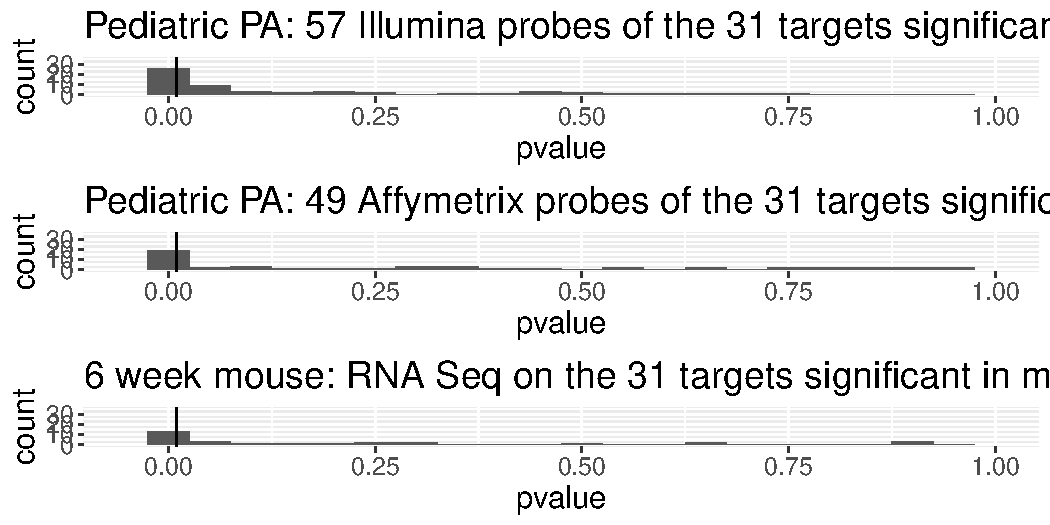
\includegraphics[width=\maxwidth]{figure/unnamed-chunk-31-1} 

\end{knitrout}
  
\end{document}
